%%%%%%%%%%%%%%%%%%%%%%%%%%%%%%%%%%%%%%%%%%%%%%%%%%%%%%%%%%%%%%%%%%%%%
% This is a LaTeX template for Bachelor or Master theses at ZHAW, in accordance with the 
% guidelines provided here:
% https://www.zhaw.ch/en/lsfm/study/studiweb/master-ls/masters-thesis/
%
%
% This template is based on previous works by:
% Steve Gunn (http://users.ecs.soton.ac.uk/srg/softwaretools/document/templates/)
% Sunil Patel (http://www.sunilpatel.co.uk/thesis-template/)
% Matteo Delucchi (https://github.com/matteodelucchi/ZHAW_thesis-template)
%
% University specific changes were made by:
% Matteo Delucchi
% Norman Juchler
% 
% Template license:
% CC BY-NC-SA 3.0 (http://creativecommons.org/licenses/by-nc-sa/3.0/)
%%%%%%%%%%%%%%%%%%%%%%%%%%%%%%%%%%%%%%%%%%%%%%%%%%%%%%%%%%%%%%%%%%%%%

%----------------------------------------------------------------------------------------
% DOCUMENT SPECIFICATION
%----------------------------------------------------------------------------------------
\documentclass[
    11pt,                      % Default font size
    oneside,                   %One-side binding. Default: Two-side binding / alternating margins
    ngerman,                   % Language. Use ngerman for German (Neue Rechtschreibung)
    singlespacing,             % Spacing option: singlespacing, onehalfspacing or doublespacing
    %nolistspacing,            % Set spacing in lists to single
    %draft,                    % Enable draft mode: no pictures, no links, overfull hboxes indicated
    liststotoc,               % Include list of figures/tables/etc in the table of contents
    %toctotoc,                 % Include the main table of contents to the table of contents
    parskip,                  % Add vertical space between paragraphs
    %nohyperref,               % Disable links in the entire document
    % helveticafont,             % Uncomment to use Helvetica font
    headsepline,               % Show a horizontal line under the header
    chapterinoneline,         % Place the chapter title and chapter number on one line
    consistentlayout,          % Have the same layout for special chapters: 
                               % declaration, abstract and acknowledgements
]{MastersDoctoralThesis}

% Uncomment the following lines to only include a subset of chapters.
% This is useful for long documents, as typesetting takes a bit of time
%\includeonly{
%    Front/titlepage,
%    Front/imprint,
%    Front/abstract,
%    %Front/declaration,
%    %Front/acknowledgements,
%    %Front/symbols,
%    Chapters/Chapter1,
%    %Chapters/Chapter2
%    }

%----------------------------------------------------------------------------------------
% PREAMBLE: PACKAGES AND CONFIGURATIONS
%----------------------------------------------------------------------------------------
% !TEX root = main.tex

%----------------------------
%   Fonts and characters
%----------------------------

% Support for special characters
\usepackage[utf8]{inputenc}    % Specify input encoding
\usepackage[T1]{fontenc}       % Specify font encoding

% Set main fonts
% Fonts catalogue: https://tug.org/FontCatalogue/
\usepackage{mathpazo}          % Use the Palatino font by default
\usepackage{beramono}          % Override the monospace/typewriter font

% ZHAW title font
% Try to load Helvetica Rounded Bold, and OpenType font.
% Loading OTF or system fonts is possible with XeLaTeX.
% If the document is compiled using pdfLaTeX, resort 
\usepackage{ifxetex}
\ifxetex
    \usepackage{fontspec}
    \newfontfamily\zhawtitlefont{Helvetica Rounded Bold}
\else
    \newcommand{\zhawtitlefont}{\scshape}
\fi

%\usepackage[scaled]{helvet}

%----------------------------
%   Environments
%----------------------------

\usepackage{caption}           % Customized caption
\usepackage{subcaption}        % Subfigure captions
\usepackage{makecell}          % Per-cell formatting in tables (\makecell)
\usepackage{pdfpages}          % Required to include PDF files/graphics (\includepdf)
\usepackage{float}             % selbst hinzugefügt

\usepackage{todonotes}         % Introduces the command \todo
\setlength{\marginparwidth}{2.5cm} % Adjust this if the todo notes are out of margins

% Create boxes as follows:
% \begin{colorbox}{red}{2}
\usepackage{tcolorbox}
\newtcolorbox{textbox}[2]{
    arc=3pt,
    boxrule=#2pt,
    colback=#1!25!white,
    width=\textwidth,
    halign=left,
    valign=center,
    colframe=#1!75!black
}

%----------------------------
%   Colors
%----------------------------

% Set up colors
\usepackage{xcolor}
% ZHAW Blue: Pantone 2945 U / R0 G100 B166
\definecolor{zhawblue}{rgb}{0.00, 0.39, 0.65}
% Colors related to code listings
\definecolor{codegreen}{rgb}{0,0.6,0}
\definecolor{codegray}{rgb}{0.5,0.5,0.5}
\definecolor{codepurple}{rgb}{0.58,0,0.82}
\definecolor{codebackground}{rgb}{0.93,0.94,0.95}

%----------------------------
%   Code listings
%----------------------------

% Setup code listings
\usepackage{listings}
\lstdefinestyle{mystyle}{
    backgroundcolor=\color{codebackground},   
    commentstyle=\color{codegreen},
    keywordstyle=\color{magenta},
    numberstyle=\tiny\color{codegray},
    stringstyle=\color{codepurple},
    basicstyle=\ttfamily\footnotesize,
    breakatwhitespace=false,
    breaklines=true,
%    captionpos=b,
    keepspaces=true,
    numbers=left,
    numbersep=5pt,
    showspaces=false,
    showstringspaces=false,
    showtabs=false,
    tabsize=4
}
\lstset{style=mystyle}

% minted is an alternative code listing package. (See chapter 2)
% For it to run successfully, ensure the following:
% - the Python package Pygments. Install with the following command:
%       python -m pip install Pygments
% - pdflatex (or xelatex) is executed with the flag --shell-escape
%   If you are using a TEX editor, you can modify the typesetting 
%   command somewhere in the settings.
%\usepackage[outputdir=build]{minted}
%\usemintedstyle{xcode}
% For fancier coloring schemes, see here:
% https://tex.stackexchange.com/questions/585582
% One could also create an own style in Pygments
% https://pygments.org/docs/styles/#creating-own-styles

%----------------------------
%   References
%----------------------------

% Set up references
\usepackage[
    backend=biber,             % Use biber backend (an external tool)
    sorting=none,              % Enumerates the reference in order of their appearance
    style=numeric-comp         % Choose here your preferred citation style
]{biblatex}
\addbibresource{quellen.bib}   % The filename of the bibliography
\usepackage[autostyle=true]{csquotes} 
                               % Required to generate language-dependent quotes 
                               % in the bibliography

%----------------------------------------------------------------------------------------
%   MARGIN SETTINGS
%----------------------------------------------------------------------------------------

\geometry{
    paper=a4paper,      % Change to letterpaper for US letter
    % inner=2.5cm,        % Inner margin
    % outer=3.8cm,        % Outer margin
    inner=3cm,        % Inner margin
    outer=3cm,        % Outer margin
    top=1.5cm,          % Top margin
    bottom=1.5cm,       % Bottom margin
    %bindingoffset=.5cm, % Binding offset
    %showframe,         % Show the type block of the page
}
\setlength{\parskip}{1em}
\usepackage{enumitem}          % Layout control for list environments (e.g, itemize)
%\setlist{noitemsep}           % Suppress extra spaces between items
%\setlist{nosep}               % Suppress spaces before/after list environments

%----------------------------------------
%   CUSTOM COMMANDS
%----------------------------------------
\setcounter{secnumdepth}{4}
\bibliography{quellen}



%----------------------------------------------------------------------------------------
% THESIS INFORMATION: MODIFY THIS SECTION!
%----------------------------------------------------------------------------------------

% The information below is used in the following parts:
% - Title page
% - Imprint
% - Abstract / Zusammenfassung
% - Meta information of PDF

\thesistitle{MVB-Sniffer}               % Thesis title,              command: \ttitle
\thesistype{Projektarbeit}              % Type of thesis (e.g. Master Thesis) \ttype
\thesisdate{20.12.2024}                 % Date of submission                  \tdate
\keywords{Manchester Decoding, Sniffer und Datalogger, Multifunction Vehicle Bus, MVB}      % Keywords for the thesis,            \keywordnames
\authorA{Noah Häuptli}                  % Your name,
\authorB{Dario Iaquinto}
\authorC{Moritz Zweifel}
\authorS{Noah Häuptli, Dario Iaquinto, Moritz Zweifel}
\degree{Bachelor of Science ZFH}            % Degree name,                        \degreename
\studyprogram{Systemtechnik}                % Study program                       \studyprog
\studyprogramlink{https://www.zhaw.ch/de/engineering/studium/bachelorstudium/systemtechnik/}    % Link to study program               \studyproglink

\supervisorA{Patrick Rennhard}             % Name of supervisor 1,               \supnameA
\supervisorAmail{patrick.rennhard@zhaw.ch}  % Email address of supervisor 1,      \supmailA
\supervisorAweb{}                           %            \supwebA
\supervisorAinfo{                       % Formatted info about supervisor 1:  \supinfoA
    \supnameA\\
    ZHAW School of Engineering\\
    Email: \href{mailto:\supmailA}{\supmailA}\\
}

% Keep empty if there is no supervisor 2: \supervisorB{}
\supervisorB{Michael Jäger}              % Name of supervisor 2,               \supnameB
\supervisorBmail{michael.jaeger@zhaw.ch}       % Email address of supervisor 2,      \supmailB
\supervisorBweb{}                  % \supwebB
\supervisorBinfo{                       % Formatted info about supervisor 2:  \supinfoB
    \supnameB\\
    ZHAW School of Engineering\\
    Email: \href{mailto:\supmailB}{\supmailB}\\
}

\university{Zurich University of Applied Sciences}
                                        % University name                     \univname
\universitygerman{Zürcher Hochschule für Angewandte Wissenschaften}
                                        % University, in German               \univnameger
\unversityabbr{ZHAW}                    % University abbreviation             \univabbr

\department{School of Engineering} 
                                        % Department,                         \deptname
\institute{Institute of Signal Processing and Wireless Communications} 
                                        % Institute,                          \instname
\group{} 
                                        % Research group                      \groupname

% Links
\universitylink      {https://www.zhaw.ch/en/university/}                   % \univlink
\universitylinkgerman{https://www.zhaw.ch/de/university/}                   % \univlinkger
\departmentlink      {https://www.zhaw.ch/de/engineering/}                         % \deptlink
\institutelink       {https://www.zhaw.ch/de/engineering/institute-zentren/isc/} % \instlink
\grouplink           {} % \grplink



\AtBeginDocument{
\hypersetup{pdftitle=\ttitle} % Set the PDF's title to your title
\hypersetup{pdfauthor=\autnameS} % Set the PDF's author to your name
\hypersetup{pdfkeywords=\keywordnames} % Set the PDF's keywords to your keywords
}

\begin{document}
\frontmatter                  % Roman page numbering for the pre-content pages
\pagestyle{plain}             % Default to the plain heading style until the thesis style 
                              % is called for the body content


%----------------------------------------------------------------------------------------
% TITLE PAGE AND IMPRINT
%----------------------------------------------------------------------------------------
% !TEX root = ../main.tex

%----------------------------------------------------------------------------------------
% APPENDIX: DECLARATION OF ORIGINALITY
%----------------------------------------------------------------------------------------

% Include the official "Plagiatserklärung" as a PDF

% Ensure that a TOC entry is create while suppressing the chapter header
\cleardoublepage
\phantomsection
%\addtocounter{chapter}{1}
%\addcontentsline{toc}{chapter}{\protect\numberline{\thechapter} Declaration of %Originality}
% The above replaces this command (which creates a chapter header).
%\chapter{Declaration of Originality} % Main appendix title
\label{DeclarationOfOriginalityZHAW}

% Include a PDF (full page)
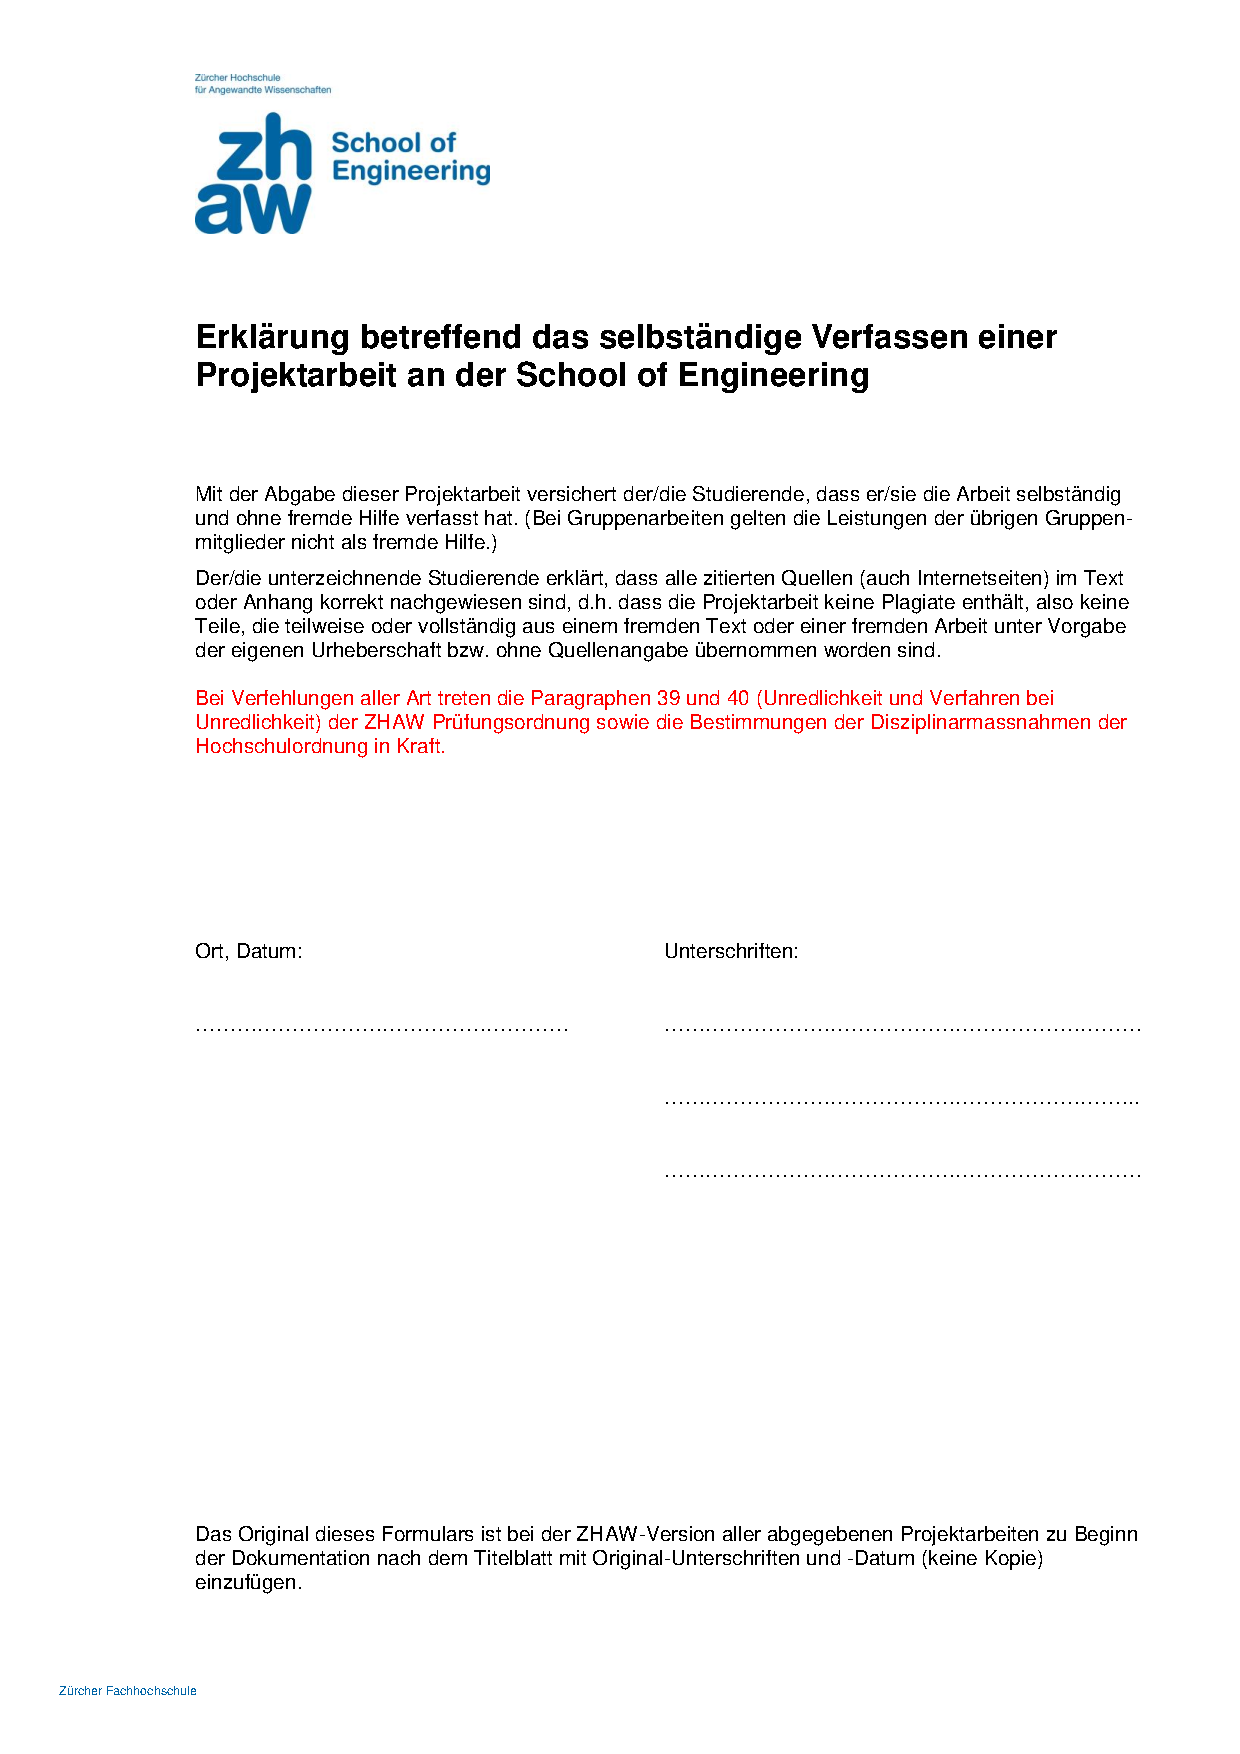
\includepdf[pages=-1]{Appendices/Erklaerung_PA.pdf}

% !TEX root = ../main.tex

%----------------------------------------------------------------------------------------
% TITLE PAGE
%----------------------------------------------------------------------------------------

\newgeometry{margin=1in}
\begin{titlepage}

% Make the title page mostly inert to the parskip-setting.
\setlength{\parskip}{0pt}

\begin{center}
\includegraphics[width=0.15\textwidth]{Figures/zhaw_rgb}

\ifxetex
    \vspace{0.6cm}
    {\zhawtitlefont\color{zhawblue}\LARGE \univname\par}   % University
    \vspace{0.2cm}
\else
    \vspace{0.87cm}
    {\includegraphics[height=17.9pt]{Figures/zhaw_font_eng_font}\par}
    \vspace{0.05cm}
\fi
{\Large Departement \deptname\par}                      % Department
\vspace{0.2cm}
{\Large \instname\par}                                 % Institute
\vspace{3.5cm}                            
\textsc{\Large \ttype}                                 % Thesis type
\vspace{0.2cm}
\HRule 
\vspace{0.4cm}
{\huge \bfseries \ttitle\par}                          % Thesis title
\vspace{0.4cm}  
\HRule
\vspace{1.5cm}

 
\begin{minipage}[t]{0.4\textwidth}
\begin{flushleft} 
    \large
    \emph{Autoren:}\\
    \autnameA\\
    \autnameB\\
    \autnameC
\end{flushleft}
\end{minipage}
\begin{minipage}[t]{0.4\textwidth}
\begin{flushright} 
    \large
    \emph{Betreuungspersonen:} \\
    \supnameA \\
    \supnameB
\end{flushright}
\end{minipage}
\vspace{2cm}
 
\vfill

{\large
Eingereicht am\\
\tdate\\
\vspace{1.5cm}
Studiengang:\\
\studyprog\\
}
\vfill
\end{center}
\end{titlepage}
\restoregeometry

\let\cleardoublepage\clearpage
%% !TEX root = ../main.tex

%----------------------------------------------------------------------------------------
% IMPRINT
%----------------------------------------------------------------------------------------

\thispagestyle{empty}
\vspace*{\fill}

{\bfseries  \Large Imprint}
\vspace{0.75cm}

\begin{footnotesize}


\begin{flushleft} 
\begin{tabular}{ @{}lp{0.6\textwidth}@{} } 
\emph{Projekt}:  & \ttype\\ 
\emph{Titel}:    & \ttitle\\
\emph{Autoren}:   & \autnameS\\
\emph{Datum}:     & \tdate\\
\emph{Schlüsselwörter}: & \keywordnames\\
\emph{Copyright}:& \univnameger

\end{tabular}
\end{flushleft}

\vspace{0.75cm}


\begin{minipage}[t]{0.95\textwidth}
\begin{flushleft} 
\emph{Studienprogramm:}\\
\href{\studyproglink}{\studyprog}\\
\href{\univlink}{\univnameger}
\end{flushleft}
\end{minipage}

\vspace{0.75cm}

\begin{minipage}[t]{0.50\textwidth}
\begin{flushleft} 
\emph{Betreuungsperson 1:}\\
\supinfoA
\end{flushleft}
\end{minipage}
\begin{minipage}[t]{0.45\textwidth}
\begin{flushleft} 
\ifdefempty{\supnameB}
{}
{
    \emph{Betreuungsperson 2:}\\
    \supinfoB
}
\end{flushleft}
\end{minipage}

\end{footnotesize}



%----------------------------------------------------------------------------------------
% DECLARATION
%----------------------------------------------------------------------------------------
% Comment out this section if the declaration of originality from ZHAW is used.
%% !TEX root = ../main.tex

%----------------------------------------------------------------------------------------
% DECLARATION OF ORIGINALITY
%----------------------------------------------------------------------------------------

\begin{declaration}
\addchaptertocentry{\authorshipname} % Add the declaration to the table of contents

\begin{textbox}{red}{2}
REMOVE THIS SECTION IF THE \href{https://www.zhaw.ch/en/lsfm/study/studiweb/master-ls/masters-thesis/}{ORIGINAL COPY OF THE ZHAW DECLARATION OF ORIGINALITY} IS USED IN THE APPENDIX.
\end{textbox}
\vspace{1cm}

\noindent We, \autnameA, \autnameB, \autnameC, declare that this thesis titled, \enquote{\ttitle} and the work presented in it are my own. I confirm that:

\begin{itemize} 
\item This work was done wholly or mainly while in candidature for a research degree at the \univname.
\item Where any part of this thesis has previously been submitted for a degree or any other qualification at this university or any other institution, this has been clearly stated.
\item Where I have consulted the published work of others, this is always clearly attributed.
\item Where I have quoted from the work of others, the source is always given. With the exception of such quotations, this thesis is entirely my own work.
\item I have acknowledged all main sources of help.
\item Where the thesis is based on work done by myself jointly with others, I have made clear exactly what was done by others and what I have contributed myself.
\end{itemize}
\vspace{1cm}

\noindent Signed:\\
\rule[0.5em]{25em}{0.5pt} % This prints a line for the signature
 
\noindent Date:\\
\rule[0.5em]{25em}{0.5pt} % This prints a line to write the date
\end{declaration}

%\cleardoublepage


%----------------------------------------------------------------------------------------
% ABSTRACT
%----------------------------------------------------------------------------------------
% !TEX root = ../main.tex

%----------------------------------------------------------------------------------------
% German ABSTRACT PAGE
%----------------------------------------------------------------------------------------
%\renewcommand{\extraabstractname}{Abstract} % muss hier bleiben, sonst ist der Titel "Zusammenfassung", weil auf Deutsch gewechselt

\begin{abstract}
%\addchaptertocentry{\abstractname} % Add the abstract to the table of contents
Die Schweizerischen Bundesbahnen (SBB) setzen Züge ein, die den Multifunction Vehicle Bus (MVB) zur Kommunikation zwischen verschiedenen Systemen nutzen. Ziel dieser Arbeit war die Entwicklung eines MVB-Sniffers, der es ermöglicht, den MVB-Datenverkehr zu erfassen und zu analysieren.

Für die Umsetzung wurde ein Transceiver, ein FPGA sowie ein Mikrocontroller ausgewählt. Der Entwicklungsprozess wurde auf Basis von Evaluationsboards gestartet. Auf einem Zug wurde eine MVB-Datenaufzeichnung durchgeführt, um den Datenverkehr zu charakterisieren und später den Aufbau und die Firmware der Evaluationsboards zu überprüfen. Der Transceiver führt die beiden MVB-Signale zusammen. Der FPGA tastet das resultierende Signal ab und dekodiert es. Anschliessend wird der Bitstream an den Mikrocontroller übertragen, der die MVB-Daten in Telegramme verpackt und per Bluetooth ausgibt. Parallel dazu wurde ein Schaltplan für den MVB-Sniffer erstellt, welcher das Hardware-Design der Evaluationsboards vereint.

Die Tests zur Datenauswertung und -übertragung im FPGA zeigten zuverlässige Ergebnisse in verschiedenen Szenarien. Die Abtast- und Auswertelogik vom FPGA funktioniert robust und fehlerfrei. Allerdings zeigt der Versuchsaufbau seine Probleme. Die SPI-Kommunikation zwischen dem FPGA und dem Mikrocontroller funktioniert nicht mit der Datenrate des realen MVB. Die Kommunikation ist nur stabil, wenn die Sendepausenzeit auf dem Bus künstlich verlängert wird.

Die SPI-Schnittstelle des gewählten Mikrocontrollers ist ungeeignet, um die volle Datenrate des MVB vom FPGA zu empfangen, da sie keine Hardware-SPI-Peripherie bietet. Somit kommt es zu fehlerhaften Transaktionen, welche vom Mikrocontroller falsch verarbeitet werden. Ebenfalls ist die Datenintegrität des FPGA-Buffers noch nicht gegeben, wodurch falsche Transaktionen ausgeführt werden.

Obwohl der Versuchsaufbau noch nicht die volle Busauslastung verarbeiten kann, resultiert eine Vielzahl von wichtigen Erkenntnissen aus dieser Arbeit. Für eine Weiterentwicklung des MVB-Sniffers erscheint es sinnvoll, den Mikrocontroller zu wechseln zu einem mit echter Hardware-SPI-Peripherie, sowie den bestehenden Buffer des FPGA zu optimieren und einen zusätzlichen einzuführen.

\end{abstract}


%----------------------------------------------------------------------------------------
% ABSTRACT PAGE
%----------------------------------------------------------------------------------------
\renewcommand{\extraabstractname}{Abstract} % muss hier bleiben, sonst ist der Titel "Zusammenfassung", weil auf Deutsch gewechselt
\begin{extraAbstract}
%\addchaptertocentry{\extraabstractname} % Add the abstract to the table of contents
The Swiss Federal Railways (SBB) use trains that utilise the Multifunction Vehicle Bus (MVB) for communication between different systems. The aim of this work was to develop an MVB sniffer that makes it possible to record and analyse MVB data traffic.

A transceiver, an FPGA and a microcontroller were selected for the implementation. The development process was started on the basis of evaluation boards. MVB data recording was carried out on a train in order to characterise the data traffic and later check the structure and firmware of the evaluation boards. The transceiver merges the two MVB signals, which are then sampled and decoded by the FPGA. The bitstream is then transmitted to the microcontroller, which packages the MVB data into telegrams and outputs them via Bluetooth. At the same time, a circuit diagram for the MVB sniffer was created, which combines the hardware design.

The tests for data evaluation and transmission in the FPGA showed reliable results in various scenarios. The FPGA's sampling and evaluation logic works robustly and without errors. However, the test setup shows its problems. The SPI communication between the FPGA and the microcontroller does not work at the data rate of the real MVB. Communication is only stable if the transmission pause time on the bus is artificially extended.

The SPI interface of the selected microcontroller is unsuitable for receiving the full data rate of the MVB from the FPGA, as it does not offer any hardware SPI peripherals. This results in incorrect transactions, which are processed incorrectly by the microcontroller. Also, the data integrity of the FPGA buffer is not yet given, resulting in incorrect transactions being executed.

Although the test setup is not yet able to process the full bus utilisation, a number of important findings have resulted from this work. For further development of the MVB sniffer, it seems sensible to change the microcontroller to one with real hardware SPI peripherals, as well as to optimise the existing FPGA buffer and introduce an additional one.

\end{extraAbstract}

%----------------------------------------------------------------------------------------
% Vorwort
%----------------------------------------------------------------------------------------
%\renewcommand{\extraabstractname}{Vorwort} 
%\begin{extraAbstract}
%\addchaptertocentry{\extraabstractname} % Add the abstract to the table of contents


%\end{extraAbstract}



%----------------------------------------------------------------------------------------
% ACKNOWLEDGEMENTS
%----------------------------------------------------------------------------------------
%% !TEX root = ../main.tex

%----------------------------------------------------------------------------------------
% ACKNOWLEDGEMENTS
%----------------------------------------------------------------------------------------
\begin{acknowledgements}
%\addchaptertocentry{\acknowledgementname} % Add the acknowledgements to the table of contents

The acknowledgements belong here. Do not forget to mention your project supervisors, without flattering them too much.
\end{acknowledgements}



%----------------------------------------------------------------------------------------
% LIST OF CONTENTS/FIGURES/TABLES PAGES
%----------------------------------------------------------------------------------------
% Comment out if any of the following is not needed:
\tableofcontents  % Add main table of contents
%\listoffigures    % Add list of figures
%\listoftables     % Add list of tables


%----------------------------------------------------------------------------------------
% ABBREVIATIONS / SYMBOLS
%----------------------------------------------------------------------------------------
%% !TEX root = ../main.tex

%----------------------------------------------------------------------------------------
% ABBREVIATIONS
%----------------------------------------------------------------------------------------

% Liste der Abkürzungen: eine zweispaltige Tabelle.
\begin{abbreviations}{ll}

\textbf{LAH} & \textbf{L}ist \textbf{A}bbreviations \textbf{H}ere\\
\textbf{WSF} & \textbf{W}hat (it) \textbf{S}tands \textbf{F}or\\

\end{abbreviations}


%----------------------------------------------------------------------------------------
% PHYSICAL CONSTANTS/OTHER DEFINITIONS
%----------------------------------------------------------------------------------------

%% List of physical constants: a three column table
%\begin{constants}{lr@{${}={}$}l} 
%
%% The \SI{}{} command is provided by the siunitx package, see its documentation 
%% for instructions on how to use it
%
%Speed of Light & $c_{0}$ & \SI{2.99792458e8}{\meter\per\second} (exact)\\
%%Constant Name & $Symbol$ & $Constant Value$ with units\\
%
%\end{constants}


%----------------------------------------------------------------------------------------
% SYMBOLS
%----------------------------------------------------------------------------------------

%% List of Symbols: a three column table
%\begin{symbols}{lll} 
%
%$a$ & distance & \si{\meter} \\
%$P$ & power & \si{\watt} (\si{\joule\per\second}) \\
%%Symbol & Name & Unit \\
%
%\addlinespace % Gap to separate the Roman symbols from the Greek
%
%$\omega$ & angular frequency & \si{\radian} \\
%
%\end{symbols}




%----------------------------------------------------------------------------------------
% THESIS CONTENT - CHAPTERS
%----------------------------------------------------------------------------------------
\mainmatter % Begin numeric (1,2,3...) page numbering
\pagestyle{thesis} % Return the page headers back to the "thesis" style


% Include the chapters of the thesis as separate files from the Chapters folder
% Uncomment the lines as you write the chapters

%% Indicate the main file. Must go at the beginning of the file.
% !TEX root = ../main.tex

%----------------------------------------------------------------------------------------
% CHAPTER 1
%----------------------------------------------------------------------------------------



\chapter{Introduction to \LaTeX} % Main chapter title
\label{Introduction} % For referencing the chapter elsewhere, use \ref{Chapter1} 

%----------------------------------------------------------------------------------------

% Define some commands to keep the formatting separated from the content
% Placing such commands in the preamble is a good idea.
\newcommand{\keyword}[1]{\textbf{#1}}
\newcommand{\tabhead}[1]{\textbf{#1}}
\newcommand{\code}[1]{\texttt{#1}}
\newcommand{\file}[1]{\texttt{\bfseries#1}}
\newcommand{\option}[1]{\texttt{\itshape#1}}

%----------------------------------------------------------------------------------------

\section{Welcome and Thank You}
Welcome to this \LaTeX{} Thesis Template, a beautiful and easy to use template for writing a thesis using the \LaTeX{} typesetting system.

If you are writing a thesis (or will be in the future) and its subject is technical or mathematical (though it doesn't have to be), then creating it in \LaTeX{} is highly recommended as a way to make sure you can just get down to the essential writing without having to worry over formatting or wasting time arguing with your word processor.

\LaTeX{} is easily able to professionally typeset documents that run to hundreds or thousands of pages long. With simple mark-up commands, it automatically sets out the table of contents, margins, page headers and footers and keeps the formatting consistent and beautiful. One of its main strengths is the way it can easily typeset mathematics, even \emph{heavy} mathematics. Even if those equations are the most horribly twisted and most difficult mathematical problems that can only be solved on a super-computer, you can at least count on \LaTeX{} to make them look stunning.

%----------------------------------------------------------------------------------------

\section{Learning \LaTeX{}}

\LaTeX{} is not a \textsc{wysiwyg} (What You See is What You Get) program, unlike word processors such as Microsoft Word or Apple's Pages. Instead, a document written for \LaTeX{} is actually a simple, plain text file that contains \emph{no formatting}. You tell \LaTeX{} how you want the formatting in the finished document by writing in simple commands amongst the text, for example, if I want to use \emph{italic text for emphasis}, I write the \verb|\emph{text}| command and put the text I want in italics in between the curly braces. This means that \LaTeX{} is a \enquote{mark-up} language, very much like HTML.

\subsection{A (not so short) Introduction to \LaTeX{}}

If you are new to \LaTeX{}, there is a very good eBook -- freely available online as a PDF file -- called, \enquote{The Not So Short Introduction to \LaTeX{}}. The book's title is typically shortened to just \emph{lshort}. You can download the latest version (as it is occasionally updated) from here:
\url{http://www.ctan.org/tex-archive/info/lshort/english/lshort.pdf}

It is also available in several other languages. Find yours from the list on this page: \url{http://www.ctan.org/tex-archive/info/lshort/}

It is recommended to take a little time out to learn how to use \LaTeX{} by creating several, small `test' documents, or having a close look at several templates on:\\ 
\url{http://www.LaTeXTemplates.com}\\ 
Making the effort now means you're not stuck learning the system when what you \emph{really} need to be doing is writing your thesis.

\subsection{A Short Math Guide for \LaTeX{}}

If you are writing a technical or mathematical thesis, then you may want to read the document by the AMS (American Mathematical Society) called, \enquote{A Short Math Guide for \LaTeX{}}. It can be found online:

\url{http://www.ams.org/tex/amslatex.html} $\rightarrow$ \enquote{Additional Documentation}\\
\url{https://mirror.foobar.to/CTAN/info/short-math-guide/}

\subsection{Common \LaTeX{} Math Symbols}
There are a multitude of mathematical symbols available for \LaTeX{} and it would take a great effort to learn the commands for them all. The most common ones you are likely to use are shown on this page:
\url{http://www.sunilpatel.co.uk/latex-type/latex-math-symbols/}

You can use this page as a reference or crib sheet, the symbols are rendered as large, high quality images so you can quickly find the \LaTeX{} command for the symbol you need.

\subsection{\LaTeX{} on a Mac}
 
The \LaTeX{} distribution is available for many systems including Windows, Linux and Mac OS X. The package for OS X is called MacTeX and it contains all the applications you need -- bundled together and pre-customized -- for a fully working \LaTeX{} environment and work flow.
 
MacTeX includes a custom dedicated \LaTeX{} editor called TeXShop for writing your `\file{.tex}' files and BibDesk: a program to manage your references and create your bibliography section just as easily as managing songs and creating playlists in iTunes.

%----------------------------------------------------------------------------------------

\section{Getting Started with this Template}

If you are familiar with \LaTeX{}, then you should explore the directory structure of the template and then proceed to place your own information into the \emph{THESIS INFORMATION} block of the \file{main.tex} file. You can then modify the rest of this file to your unique specifications based on your degree/university. Section \ref{FillingFile} on page \pageref{FillingFile} will help you do this. Make sure you also read section \ref{ThesisConventions} about thesis conventions to get the most out of this template.

If you are new to \LaTeX{} it is recommended that you carry on reading through the rest of the information in this document.

Before you begin using this template you should ensure that its style complies with the thesis style guidelines imposed by your institution. In most cases this template style and layout will be suitable. If it is not, it may only require a small change to bring the template in line with your institution's recommendations. These modifications will need to be done on the \file{MastersDoctoralThesis.cls} file.

\subsection{About this Template}

This \LaTeX{} Thesis Template is originally based and created around a \LaTeX{} style file created by Steve R.\ Gunn from the University of Southampton (UK), department of Electronics and Computer Science. You can find his original thesis style file at his site, here:
\url{http://www.ecs.soton.ac.uk/~srg/softwaretools/document/templates/}

Steve's \file{ecsthesis.cls} was then taken by Sunil Patel who modified it by creating a skeleton framework and folder structure to place the thesis files in. The resulting template can be found on Sunil's site here:
\url{http://www.sunilpatel.co.uk/thesis-template}


Sunil's template was made available through \url{http://www.LaTeXTemplates.com}, where it was modified many times based on user requests and questions. Version 2.0 and onwards of this template represents a major modification to Sunil's template and is, in fact, hardly recognisable. The work to make version 2.0 possible was carried out by \href{mailto:vel@latextemplates.com}{Vel} and Johannes Böttcher.

Based on Sunil's Version 2.0, Matteo updated the template and incorporated ZHAW University thesis guidelines.

%----------------------------------------------------------------------------------------

\section{What this Template Includes}

\subsection{Folders}

This template comes as a single zip file that expands out to several files and folders. The folder names are mostly self-explanatory:

\keyword{Appendices} -- this is the folder where you put the appendices. Each appendix should go into its own separate \file{.tex} file. An example and template are included in the directory.

\keyword{Chapters} -- this is the folder where you put the thesis chapters. A thesis usually has about six chapters, though there is no hard rule on this. Each chapter should go in its own separate \file{.tex} file and they can be split as:
\begin{itemize}
\item Chapter 1: Introduction to the thesis topic
\item Chapter 2: Background information and theory
\item Chapter 3: (Laboratory) experimental setup
\item Chapter 4: Details of experiment 1
\item Chapter 5: Details of experiment 2
\item Chapter 6: Discussion of the experimental results
\item Chapter 7: Conclusion and future directions
\end{itemize}
This chapter layout is specialised for the experimental sciences, your discipline may be different.

\keyword{Figures} -- this folder contains all figures for the thesis. These are the final images that will go into the thesis document.

\subsection{Files}

Included are also several files, most of them are plain text and you can see their contents in a text editor. After initial compilation, you will see that more auxiliary files are created by \LaTeX{} or BibTeX and which you don't need to delete or worry about:

\keyword{example.bib} -- this is an important file that contains all the bibliographic information and references that you will be citing in the thesis for use with BibTeX. You can write it manually, but there are reference manager programs available that will create and manage it for you. Bibliographies in \LaTeX{} are a large subject and you may need to read about BibTeX before starting with this. Many modern reference managers will allow you to export your references in BibTeX format which greatly eases the amount of work you have to do.

\keyword{MastersDoctoralThesis.cls} -- this is an important file. It is the class file that tells \LaTeX{} how to format the thesis. 

\keyword{main.pdf} -- this is your beautifully typeset thesis (in the PDF file format) created by \LaTeX{}. It is supplied in the PDF with the template and after you compile the template you should get an identical version.

\keyword{main.tex} -- this is an important file. This is the file that you tell \LaTeX{} to compile to produce your thesis as a PDF file. It contains the framework and constructs that tell \LaTeX{} how to layout the thesis. It is heavily commented so you can read exactly what each line of code does and why it is there. After you put your own information into the \emph{THESIS INFORMATION} block -- you have now started your thesis!

Files that are \emph{not} included, but are created by \LaTeX{} as auxiliary files include:

\keyword{main.aux} -- this is an auxiliary file generated by \LaTeX{}, if it is deleted \LaTeX{} simply regenerates it when you run the main \file{.tex} file.

\keyword{main.bbl} -- this is an auxiliary file generated by BibTeX, if it is deleted, BibTeX simply regenerates it when you run the \file{main.aux} file. Whereas the \file{.bib} file contains all the references you have, this \file{.bbl} file contains the references you have actually cited in the thesis and is used to build the bibliography section of the thesis.

\keyword{main.blg} -- this is an auxiliary file generated by BibTeX, if it is deleted BibTeX simply regenerates it when you run the main \file{.aux} file.

\keyword{main.lof} -- this is an auxiliary file generated by \LaTeX{}, if it is deleted \LaTeX{} simply regenerates it when you run the main \file{.tex} file. It tells \LaTeX{} how to build the \emph{List of Figures} section.

\keyword{main.log} -- this is an auxiliary file generated by \LaTeX{}, if it is deleted \LaTeX{} simply regenerates it when you run the main \file{.tex} file. It contains messages from \LaTeX{}, if you receive errors and warnings from \LaTeX{}, they will be in this \file{.log} file.

\keyword{main.lot} -- this is an auxiliary file generated by \LaTeX{}, if it is deleted \LaTeX{} simply regenerates it when you run the main \file{.tex} file. It tells \LaTeX{} how to build the \emph{List of Tables} section.

\keyword{main.out} -- this is an auxiliary file generated by \LaTeX{}, if it is deleted \LaTeX{} simply regenerates it when you run the main \file{.tex} file.

So from this long list, only the files with the \file{.bib}, \file{.cls} and \file{.tex} extensions are the most important ones. The other auxiliary files can be ignored or deleted as \LaTeX{} and BibTeX will regenerate them.

%----------------------------------------------------------------------------------------

\section{Filling in Your Information in the \file{main.tex} File}\label{FillingFile}

You will need to personalise the thesis template and make it your own by filling in your own information. This is done by editing the \file{main.tex} file in a text editor or your favourite LaTeX environment.

Open the file and scroll down to the third large block titled \emph{THESIS INFORMATION} where you can see the entries for \emph{University Name}, \emph{Department Name}, etc \ldots

Fill out the information about yourself, your group and institution. You can also insert web links, if you do, make sure you use the full URL, including the \code{http://} for this. If you don't want these to be linked, simply remove the \verb|\href{url}{name}| and only leave the name.

When you have done this, save the file and recompile \code{main.tex}. All the information you filled in should now be in the PDF, complete with web links. You can now begin your thesis proper!

%----------------------------------------------------------------------------------------

\section{The \code{main.tex} File Explained}

The \file{main.tex} file contains the structure of the thesis. There are plenty of written comments that explain what pages, sections and formatting the \LaTeX{} code is creating. Each major document element is divided into commented blocks with titles in all capitals to make it obvious what the following bit of code is doing. Initially there seems to be a lot of \LaTeX{} code, but this is all formatting, and it has all been taken care of so you don't have to do it.

Begin by checking that your information on the title page is correct. For the thesis declaration, your institution may insist on something different than the text given. If this is the case, just replace what you see with what is required in the \emph{DECLARATION PAGE} block.

Then comes a page which contains a funny quote. You can put your own, or quote your favourite scientist, author, person, and so on. Make sure to put the name of the person who you took the quote from.

Following this is the abstract page which summarises your work in a condensed way and can almost be used as a standalone document to describe what you have done. The text you write will cause the heading to move up so don't worry about running out of space.

Next come the acknowledgements. On this page, write about all the people who you wish to thank (not forgetting parents, partners and your advisor/supervisor).

The contents pages, list of figures and tables are all taken care of for you and do not need to be manually created or edited. The next set of pages are more likely to be optional and can be deleted since they are for a more technical thesis: insert a list of abbreviations you have used in the thesis, then a list of the physical constants and numbers you refer to and finally, a list of mathematical symbols used in any formulae. Making the effort to fill these tables means the reader has a one-stop place to refer to instead of searching the internet and references to try and find out what you meant by certain abbreviations or symbols.

The list of symbols is split into the Roman and Greek alphabets. Whereas the abbreviations and symbols ought to be listed in alphabetical order (and this is \emph{not} done automatically for you) the list of physical constants should be grouped into similar themes.

The next page contains a one line dedication. Who will you dedicate your thesis to?

Finally, there is the block where the chapters are included. Uncomment the lines (delete the \code{\%} character) as you write the chapters. Each chapter should be written in its own file and put into the \emph{Chapters} folder and named \file{Chapter1}, \file{Chapter2}, etc\ldots Similarly for the appendices, uncomment the lines as you need them. Each appendix should go into its own file and placed in the \emph{Appendices} folder.

After the preamble, chapters and appendices finally comes the bibliography. The bibliography style (called \option{authoryear}) is used for the bibliography and is a fully featured style that will even include links to where the referenced paper can be found online. Do not underestimate how grateful your reader will be to find that a reference to a paper is just a click away. Of course, this relies on you putting the URL information into the BibTeX file in the first place.

%----------------------------------------------------------------------------------------

\section{Thesis Features and Conventions}\label{ThesisConventions}

To get the best out of this template, there are a few conventions that you may want to follow.

One of the most important (and most difficult) things to keep track of in such a long document as a thesis is consistency. Using certain conventions and ways of doing things (such as using a Todo list) makes the job easier. Of course, all of these are optional and you can adopt your own method.

\subsection{Printing Format}

This thesis template is designed for double sided printing (i.e. content on the front and back of pages) as most theses are printed and bound this way. To switch to one sided printing, uncomment the \option{oneside} option of the \code{documentclass} command at the top of the \file{main.tex} file. You may then wish to adjust the margins to suit specifications from your institution.

The headers for the pages contain the page number on the outer side (so it is easy to flick through to the page you want) and the chapter name on the inner side.

The text is set to 11 point by default with single line spacing, again, you can tune the text size and spacing should you want or need to using the options at the very start of \file{main.tex}. The spacing can be changed similarly by replacing the \option{singlespacing} with \option{onehalfspacing} or \option{doublespacing}.

\subsection{Using US Letter Paper}

The paper size used in the template is A4, which is the standard size in Europe. If you are using this thesis template elsewhere and particularly in the United States, then you may have to change the A4 paper size to the US Letter size. This can be done in the margins settings section in \file{main.tex}.

Due to the differences in the paper size, the resulting margins may be different to what you like or require (as it is common for institutions to dictate certain margin sizes). If this is the case, then the margin sizes can be tweaked by modifying the values in the same block as where you set the paper size. Now your document should be set up for US Letter paper size with suitable margins.

\subsection{References}

The \code{biblatex} package is used to format the bibliography and inserts references such as this one \parencite{Reference1}. 
The inline citation style can be changed to e.g. authoryear in the \file{main.tex} file. 
\href{https://www.overleaf.com/learn/latex/Biblatex_citation_styles}{This documentation} lists and explains different standard citation styles.
The options used in the \file{main.tex} file mean that the in-text citations of references are formatted with the author(s) listed with the date of the publication. Multiple references are separated by semicolons (e.g. \parencite{Reference2, Reference1}) and references with more than three authors only show the first author with \emph{et al.} indicating there are more authors (e.g. \parencite{Reference3}). This is done automatically for you. To see how you use references, have a look at the \file{Chapter1.tex} source file. Many reference managers allow you to simply drag the reference into the document as you type.

Scientific references should come \emph{before} the punctuation mark if there is one (such as a comma or period). The same goes for footnotes\footnote{Such as this footnote, here down at the bottom of the page.}. You can change this but the most important thing is to keep the convention consistent throughout the thesis. Footnotes themselves should be full, descriptive sentences (beginning with a capital letter and ending with a full stop). The APA6 states: \enquote{Footnote numbers should be superscripted, [...], following any punctuation mark except a dash.} The Chicago manual of style states: \enquote{A note number should be placed at the end of a sentence or clause. The number follows any punctuation mark except the dash, which it precedes. It follows a closing parenthesis.}

The bibliography is typeset with references listed in alphabetical order by the first author's last name. This is similar to the APA referencing style. To see how \LaTeX{} typesets the bibliography, have a look at the very end of this document (or just click on the reference number links in in-text citations).

\subsubsection{A Note on bibtex}

The bibtex backend used in the template by default does not correctly handle unicode character encoding (i.e. "international" characters). You may see a warning about this in the compilation log and, if your references contain unicode characters, they may not show up correctly or at all. The solution to this is to use the biber backend instead of the outdated bibtex backend. This is done by finding this in \file{main.tex}: \option{backend=bibtex} and changing it to \option{backend=biber}. You will then need to delete all auxiliary BibTeX files and navigate to the template directory in your terminal (command prompt). Once there, simply type \code{biber main} and biber will compile your bibliography. You can then compile \file{main.tex} as normal and your bibliography will be updated. An alternative is to set up your LaTeX editor to compile with biber instead of bibtex, see \href{http://tex.stackexchange.com/questions/154751/biblatex-with-biber-configuring-my-editor-to-avoid-undefined-citations/}{here} for how to do this for various editors.

\subsection{Tables}

Tables are an important way of displaying your results, below is an example table which was generated with this code:

{\small
    \begin{verbatim}
    \begin{table}
    \caption{The effects of treatments X and Y 
            on the four groups studied.}
    \label{tab:treatments}
    \centering
    \begin{tabular}{l l l}
    \toprule
    \tabhead{Groups} & \tabhead{Treatment X} & \tabhead{Treatment Y} \\
    \midrule
    1 & 0.2 & 0.8\\
    2 & 0.17 & 0.7\\
    3 & 0.24 & 0.75\\
    4 & 0.68 & 0.3\\
    \bottomrule\\
    \end{tabular}
    \end{table}
    \end{verbatim}
}

\begin{table}
\caption{The effects of treatments X and Y on the four groups studied.}
\label{tab:treatments}
\centering
\begin{tabular}{l l l}
\toprule
\tabhead{Groups} & \tabhead{Treatment X} & \tabhead{Treatment Y} \\
\midrule
1 & 0.2 & 0.8\\
2 & 0.17 & 0.7\\
3 & 0.24 & 0.75\\
4 & 0.68 & 0.3\\
\bottomrule\\
\end{tabular}
\end{table}

You can reference tables with \verb|\ref{<label>}| where the label is defined within the table environment. See \file{Chapter1.tex} for an example of the label and citation (e.g. Table~\ref{tab:treatments}).

\subsection{Figures}

There will hopefully be many figures in your thesis (that should be placed in the \emph{Figures} folder). The way to insert figures into your thesis is to use a code template like this:
\begin{verbatim}
\begin{figure}
\centering

\includegraphics{Figures/Electron}
\decoRule
\caption[An Electron]{An electron (artist's impression).}
\label{fig:Electron}
\end{figure}
\end{verbatim}
Also look in the source file. Putting this code into the source file produces the picture of the electron that you can see in the figure below.

\begin{figure}[th]
\centering

\includegraphics{Figures/Electron}
\decoRule
\caption[An Electron]{An electron (artist's impression).}
\label{fig:Electron}
\end{figure}

Sometimes figures don't always appear where you write them in the source. The placement depends on how much space there is on the page for the figure. Sometimes there is not enough room to fit a figure directly where it should go (in relation to the text) and so \LaTeX{} puts it at the top of the next page. Positioning figures is the job of \LaTeX{} and so you should only worry about making them look good!

Figures usually should have captions just in case you need to refer to them (such as in Figure~\ref{fig:Electron}). The \verb|\caption| command contains two parts, the first part, inside the square brackets is the title that will appear in the \emph{List of Figures}, and so should be short. The second part in the curly brackets should contain the longer and more descriptive caption text.

The \verb|\decoRule| command is optional and simply puts an aesthetic horizontal line below the image. If you do this for one image, do it for all of them.

\LaTeX{} is capable of using images in pdf, jpg and png format.

\subsection{Typesetting mathematics}

If your thesis is going to contain heavy mathematical content, be sure that \LaTeX{} will make it look beautiful, even though it won't be able to solve the equations for you.

The \enquote{Not So Short Introduction to \LaTeX} (available on \href{http://www.ctan.org/tex-archive/info/lshort/english/lshort.pdf}{CTAN}) should tell you everything you need to know for most cases of typesetting mathematics. If you need more information, a much more thorough mathematical guide is available from the AMS called, \enquote{A Short Math Guide to \LaTeX} and can be downloaded from:
\url{ftp://ftp.ams.org/pub/tex/doc/amsmath/short-math-guide.pdf}

There are many different \LaTeX{} symbols to remember, luckily you can find the most common symbols in \href{http://ctan.org/pkg/comprehensive}{The Comprehensive \LaTeX~Symbol List}.

You can write an equation, which is automatically given an equation number by \LaTeX{} like this:
\begin{verbatim}
\begin{equation}
E = mc^{2}
\label{eqn:Einstein}
\end{equation}
\end{verbatim}

This will produce Einstein's famous energy-matter equivalence equation:
\begin{equation}
E = mc^{2}
\label{eqn:Einstein}
\end{equation}

All equations you write (which are not in the middle of paragraph text) are automatically given equation numbers by \LaTeX{}. If you don't want a particular equation numbered, use the unnumbered form:
\begin{verbatim}
\[ a^{2}=4 \]
\end{verbatim}

%----------------------------------------------------------------------------------------

\section{Sectioning and Subsectioning}

You should break your thesis up into nice, bite-sized sections and subsections. \LaTeX{} automatically builds a table of contents by looking at all \verb|\chapter{}|, \verb|\section{}|  and \verb|\subsection{}| commands you write in the source.

The Table of Contents should only list the sections to three (3) levels. A \verb|chapter{}| is level zero (0). A \verb|\section{}| is level one (1) and so a \verb|\subsection{}| is level two (2). In your thesis it is likely that you will even use a \verb|subsubsection{}|, which is level three (3). The depth to which the Table of Contents is formatted is set within \file{MastersDoctoralThesis.cls}. If you need this changed, you can do it in \file{main.tex}.

%----------------------------------------------------------------------------------------

\section{In Closing}

You have reached the end of this mini-guide. You can now rename or overwrite this pdf file and begin writing your own \file{Chapter1.tex} and the rest of your thesis. The easy work of setting up the structure and framework has been taken care of for you. It's now your job to fill it out!

Good luck and have lots of fun!

\begin{flushright}
Guide written by ---\\
Sunil Patel: \href{http://www.sunilpatel.co.uk}{www.sunilpatel.co.uk}\\
Vel: \href{http://www.LaTeXTemplates.com}{LaTeXTemplates.com}
\end{flushright}

%% Indicate the main file. Must go at the beginning of the file.
% !TEX root = ../main.tex

%----------------------------------------------------------------------------------------
% CHAPTER 2
%----------------------------------------------------------------------------------------

\chapter{Code Listings}

\label{Code Listings} % For referencing the chapter elsewhere, use \ref{Chapter2} 

%----------------------------------------------------------------------------------------

The package \href{https://www.overleaf.com/learn/latex/Code\_listing}{\code{listings}} permits to easily include existing code. Simply use the command \verb|\lstinputlisting[language=name]{path/to/file}|. See \href{https://www.overleaf.com/learn/latex/Code\_listing#Supported\_languages}{here} for a list of supported programming languages.


\lstinputlisting[language=Python,caption=External file: code/example.py]{Code/example.py}

It is also possible to enter code directly into \LaTeX:

\begin{lstlisting}[language=Matlab]
#include <stdio>
void hello_world(void){
   std::cout << "Hello World!" << std::endl;
}    
\end{lstlisting}

Alternatively, one can use the syntax highlighting toolbox \href{https://pygments.org/}{\code{Pygments}} in combination with the \LaTeX-package \href{www.overleaf.com/learn/latex/Code\_Highlighting\_with\_minted}{\code{minted}}. It provides slightly better results, as the code will actually be parsed.

To install Pygments, use the following command. For \code{minted} to work properly, run the pdflatex tool with the flag \code{--shell-escape}. If you are using a TEX editor, you can modify the typesetting   command somewhere in the settings.

\begin{lstlisting}[language=bash]
# Make sure that Pygments is installed.
python -m pip install pygments

# Then add the --shell-escape flag to the command 
# that is used to compile your LaTeX code.
pdflatex --output-dir="$BUILD_DIR" \
         --file-line-error \
         --shell-escape \
         --synctex=1 "$1"
\end{lstlisting}



% Set the following line to \iftrue if minted is available on your system.
% See the above instructions to see how.

\iffalse
See below how the result looks like if minted is available on your system.

\begin{listing}[!ht]
\inputminted[linenos, bgcolor=codebackground, style=friendly]{python}{Code/example.py}
\caption{Example from external file, parsed using \code{Pygments}}
\end{listing}

\fi 

% !TEX root = ../main.tex

% Indicate the main file. Must go at the beginning of the file.

%----------------------------------------------------------------------------------------
% CHAPTER TEMPLATE
%----------------------------------------------------------------------------------------
\chapter{Einleitung} % Main chapter title
\label{Einleitung}
Im folgenden Kapitel werden die Ausgangslage, die Aufgabenstellung und das Ziel dieser Projektarbeit erläutert.

%--------------------------------------------------------------------------------
% SECTION Problemstellung
%--------------------------------------------------------------------------------
\section{Ausgangslage} %eventuell Ausgangslage nennen!
\label{Ausgangslage} % Change X to a consecutive number

%% Text hier

Die Schweizerischen Bundesbahnen (SBB) betreiben eine umfangreiche Flotte von Schienenfahrzeugen, die verschiedene Kommunikationssysteme nutzen. Der Multifunction Vehicle Bus (MVB) ist eines dieser Systeme und ermöglicht die Datenübertragung zwischen den elektronischen Komponenten und Systemen eines Zuges.

Trotz der Robustheit des MVB können komplexe Störungen auftreten, die den Betrieb beeinträchtigen. Ein zentraler Grund für die Entwicklung eines MVB-Sniffers ist die Notwendigkeit, diese Störungen präzise zu identifizieren und zu analysieren. Ein Sniffer ist ein Gerät, welches Datenverkehr erfassen kann und durch die Aufzeichnung der Kommunikationsprotokolle ermöglicht, Probleme wie Kommunikationsausfälle zu diagnostizieren.

Ein weiterer Grund für den Einsatz eines MVB-Sniffers ist die Beobachtung und Überwachung spezifischer MVB-Teilnehmer. Bestimmte Komponenten oder Systeme innerhalb eines Zuges können aufgrund ihrer kritischen Funktion oder ihrer Anfälligkeit für Störungen eine besondere Aufmerksamkeit erfordern. Die detaillierte Analyse des MVB fördert auch ein vertieftes Verständnis des Systems.

Der MVB wird durch die Norm SN EN 61375-3-1 geregelt. Diese Norm beschreibt die grundlegenden Funktionsweisen und technischen Anforderungen des Kommunikationsprotokolls. Ergänzend dazu werden spezifische Aspekte des Linklayers auch in der Norm SN EN 61375-2-1, die den Wire Train Bus (WTB) behandelt, erläutert. Beide Normen bilden die Grundlage wie der MVB funktioniert. Die Präsentiation im Anhang \ref{app:File11} \textit{a fieldbus case study von Prof. Dr. H. Kirrmann} bietet einen vertieften und anschaulichen Überblick.
\newpage

%---------------------------------------------------------------------------------
% SECTION Aufgabenstellung
%---------------------------------------------------------------------------------

\section{Aufgabenstellung}
\label{Aufgabenstellung} % Change X to a consecutive number

%% Text hier
Die nachfolgende Liste ist ein Orientierung und umfasst nicht alle notwendigen Einzelschritte. Die Reihenfolge der Schritte kann variieren und Änderungen oder das Weglassen von Schritten muss mit den betreuenden Personen besprochen werden. Im Rahmen der Projektarbeit fanden wöchentliche Sitzungen (Sitzungsprotokolle in Anhang \ref{app:File12}) statt, in denen über den aktuellen Stand und die aktuellen Probleme informiert wurde.
 \begin{enumerate}
     \item Machen Sie sich mit dem Thema vertraut
     \item Analyse der Anforderungen an den MVB-Sniffer mit Schwerpunkt bei der Elektronik 
     \item Kleine Recherche zu kommerziell erhältlichen MVB-Sniffern
     \item Erstellen eines Zeit- und Projektplans für die verschiedenen zu erledigenden Arbeiten
     \item Erstellung eines Grobkonzeptes
     \item Hardware-Entwicklung: Auswahl geeigneter Hardwarekomponenten und Aufbau eines 
     Funktionsmusters. In einem ersten Schritt wo möglich basierend auf Evaluation-Boards und nur wo 
     nötig basierend auf eigenen Elektronik-Platinen (PCBs)
     \item Firmware-Entwicklung: Implementierung der Firmware für die Bitstrom-Decodierung
     \item Tests mit dem «MVB-Bus-Simulator»
     \item Bei raschem Voranschreiten: 
     
a. Weiterentwicklung des Funktionsmuster zu einem Prototyp 

b. Auswertung des decodierten Bitstroms zu Daten-Paketen 

c. Benutzeroberfläche zur Visualisierung der aufgezeichneten Daten 
     \item Dokumentieren Sie alle Arbeitsschritte und verfassen Sie einen wissenschaftlichen Bericht, welcher Theorie, Methodik, Resultate und Diskussion beschreibt.
     \end{enumerate}

Die ausgehändigte Aufgabenstellung befindet sich im Anhang \ref{app:Aufgabenstellung}.

%---------------------------------------------------------------------------------
% SECTION "Ziel der Arbeit"
%---------------------------------------------------------------------------------

\section{Ziel der Arbeit}
\label{Ziel der Arbeit} % Change X to a consecutive number

%% Text hier
Das Hauptziel dieser Projektarbeit ist die Entwicklung eines MVB-Sniffers für die SBB, der Kommunikationsprotokolle in MVB-Netzwerken aufzeichnen kann. Zunächst wird ein Funktionsmuster auf Basis von Evaluationsboards erstellt und zu einem späteren Zeitpunkt soll eine eigene Elektronikplatine (PCB) entwickelt werden. Im Verlaufe der Projektarbeit wurde das Minimal Value Product definiert, siehe Tabelle \ref{tab:minvalueproduct}, um klare Ziele für das Ende der Projektarbeit festzulegen.
\begin{table}[H]
\centering
\begin{tabular}{|p{1cm}|p{13cm}|}
\hline
\textbf{Level} & \textbf{Beschreibung} \\ \hline
0 Minimum Value & 
Sniffer-Aufbau auf Evaluationsboards übersetzt MVB-Telegramme und gibt diese über Bluetooth aus, visualisierbar mit einer BLE GATT-Browser-App. Ein eigenes PCB wurde in Altium (Schematics, PCB, 3D-Modell) erstellt, jedoch noch nicht getestet. Zeitstempel des FPGAs ist relativ zur Aufstartzeit. \\ \hline
1 & 
Höhere Datenrate bei der Übersetzung von MVB-Telegrammen. Erste Tests auf einem Zug durchgeführt, Erkenntnisse daraus gewonnen. Eigenes PCB ist bestellt, jedoch noch nicht getestet. \\ \hline
2 & 
Eigenes PCB ist erstellt, bestellt und getestet. Integration der Software steht noch aus. \\ \hline
3 & 
Software ist auf dem eigenen PCB implementiert und wurde mit aufgezeichneten MVB-Telegrammen getestet. \\ \hline
4 & 
Der Datenaustausch zwischen ESP und FPGA wurde erweitert. Ein aktueller Zeitstempel wird übertragen. \\ \hline
\end{tabular}
\caption{Entwicklungsstufen des Minimal Value Product (MVP)}
\label{tab:minvalueproduct}
\end{table}

%---------------------------------------------------------------------------------
% SECTION "Ziel der Arbeit"
%---------------------------------------------------------------------------------

\section{Aufbau der Arbeit}
\label{Aufbau der Arbeit} % Change X to a consecutive number
Diese Arbeit ist in vier Kapitel gegliedert, die im Folgenden vorgestellt und kurz beschrieben werden:

\textbf{Einleitung}\\
In der Einleitung folgt noch eine Einführung zu Sniffer Devices und eine Übersicht zur durchgeführten Recherche zu den bestehenden Geräten.

\textbf{Theoretische Grundlagen}\\
Im Kapitel \textit{Theoretische Grundlagen} wird der Aufbau des MVB, sowie die Funktionsweise der Datenübertragung erläutert.

\textbf{Methode}\\
Das Kapitel \textit{Methode} beschreibt in chronologischer Reihenfolge die Entwicklung des Sniffers. Zuerst wird die Messung und Auswertung zur Bestimmung der Busauslastung erklärt. Es wird dargestellt, wie der Sniffer gestaltet sein muss, um alle Anforderungen zu erfüllen. Ein weiteres Unterkapitel widmet sich der Wahl der Hardware. Abschliessend wird die Umsetzung der Logik im FPGA, der Software auf dem ESP32, sowie des Schemas beschrieben.

\textbf{Prototyp Sniffer}\\
Im Kapitel \textit{Prototyp Sniffer} werden die im Zuge der ersten Umsetzung aufgetretenen Probleme sowie entsprechende Lösungsansätze behandelt. Zudem wird der Testprozess dokumentiert und die erhaltenen Resultate werden vorgestellt.

\textbf{Diskussion und Ausblick}\\
Im letzten Kapitel \textit{Diskussion und Ausblick} werden die erreichten und nicht erreichten Ziele den zu Beginn festgelegten Erwartungen gegenübergestellt und reflektiert. Abschliessend wird ein Ausblick auf die Weiterentwicklung des MVB-Sniffers im Rahmen der Bachelorarbeit gegeben.\\
\\
\textit{Es sei erwähnt, dass in dieser Arbeit das generative KI-Tool ChatGPT für Textformulierungen, Rechtschreibkorrekturen und für die Generierung von Code verwendet wurde.}

%\chapter{Methode} % Main chapter title
%\label{chapter3:Methode} % Change X to a consecutive number; for referencing this chapter elsewhere, use \ref{ChapterX}


%-----------------------------------
% SUBSECTION "Sniffer"
%-----------------------------------

\section{Sniffer Device}
% \textcolor{red}{Was ist ein Sniffer}\\
% Ein Sniffer ist grundsätzlich ein Gerät oder ein Software-Tool welches die Kommunikation zweier oder mehrerer Geräten überwachen und aufzeichnen kann.

% Ein solcher Sniffer wird Beispielsweise oft eingesetzt um den Netzwerkverkehr zu überwachen. Ein bekanntes Beispiel eines Sniffers dieser Art ist die Sniffer-Software Wireshark.\\

% Der Sniffer wie er auch in dieser Projektarbeit entwickelt wird, ist Physisch und wird direkt an einen Datenbus gehängt um von diesem lesen zu können.
% Dabei fängt der Sniffer die versendeten Datenpakete auf dem Bus ab ohne jegliche Störungen oder
% Einschränkungen der Kommunikation der Geräte zu verursachen.

Ein Sniffer ist ein Gerät oder Software-Tool, das in der Lage ist, die Kommunikation zwischen zwei oder mehreren Geräten zu überwachen und aufzuzeichnen. Diese Art von Werkzeug wird häufig verwendet um den Datenverkehr in Netzwerken oder auf Kommunikationsbussen zu analysieren.

Ein bekanntes Beispiel für ein solches Sniffer-Tool ist die Software Wireshark, die weit verbreitet zur Überwachung von Netzwerkprotokollen eingesetzt wird.

Im Rahmen dieser Projektarbeit wird ein physischer Sniffer entwickelt, der direkt an einen Datenbus angeschlossen wird, um die auf dem Bus übertragenen Datenpakete zu lesen. Dabei agiert der Sniffer passiv und erfasst die übertragenen Daten ohne die Kommunikation zwischen den Geräten zu beeinflussen
oder zu stören.

%--------------------------------------------------------------------------------
% SECTION Stand von Konkurenzprodukten
%--------------------------------------------------------------------------------

\section{Recherche bestehende Produkte}
\label{sec:recherche}

In einer Recherche zu bereits auf dem Markt vorhandenen MVB-Sniffern wurden verschiedene Varianten
gefunden. Teilweise wurden Anforderungen, die an den zu entwickelten Sniffer gestellt wurden, erfüllt.
Es wurden drei Geräte gefunden welche in diesem Kapitel etwas näher vorgestellt werden. In den folgenden Abschnitten sind dazu die verschiedenen Geräte mit dessen Merkmalen aufgelistet. Abschliessend wird in diesem Unterkapitel darauf eingegangen was den Sniffer, welcher entwickelt werden soll, ausmacht und welchen Vorteil dieser in der künftigen Anwendung bringen soll.

%\textbf{Sniffer 1: AMiT MVB Analyzer RB-MVB/AN01}\\[2ex]
\begin{minipage}{0.4\textwidth}
  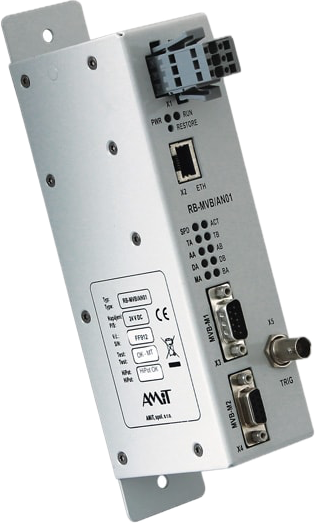
\includegraphics[width=0.7\linewidth]{Figures/Chap3/Konkurenz/Amit.png}
  \captionof{figure}{\mbox{AMiT MVB Analyzer \cite{Amit}}}
  \label{fig:AmitAnalyzer}
\end{minipage}
\hfill
\begin{minipage}{0.57\textwidth}
  \begin{tabular}{|m{3.3cm}|m{4.2cm}|}
  \hline
    \multicolumn{2}{|c|}{\textbf{AMiT MVB Analyzer RB-MVB/AN01}} \\ \hline
    \textbf{Firma} & AMiT Transportation \\ \hline
    \textbf{Datenbus} & MVB (EMD/ESD Kapitel \ref{Übertragungsmedien}) \\ \hline
    \textbf{Datenraten} & MVB: 1,5 Mbps / Ethernet: 10/100 Mbps \\ \hline
    \textbf{Galvanische \mbox{Trennung}} & nur Ethernet \\ \hline
    \textbf{Schnittstellen} & MVB: D-Sub 9 Pol / Ethernet: RJ45 \\ \hline
    \textbf{Stromversorgung} & 16.8–33.6 V DC \\ \hline
    \textbf{Einsatztemperatur} & -40 °C bis 70 °C \\ \hline
    \textbf{Schutzart} & IP20 \\ \hline
    \textbf{Gewicht} & 0.9 kg \\ \hline
    \textbf{Abmessungen} & 33 × 228 × 87 mm \\ \hline
    \textbf{Software} & Wireshark-Plug-in \\ \hline
    \textbf{Besonderheiten} & Redundantes MVB Interface (A und B Kapitel \ref{Übertragungsmedien}) \\ \hline
  \end{tabular}

\end{minipage}

%\textbf{Sniffer 2: Ci4Rail ModuSio MIO03 MVB/CAN Sniffer}\\[2ex]
\begin{minipage}{0.4\textwidth}
  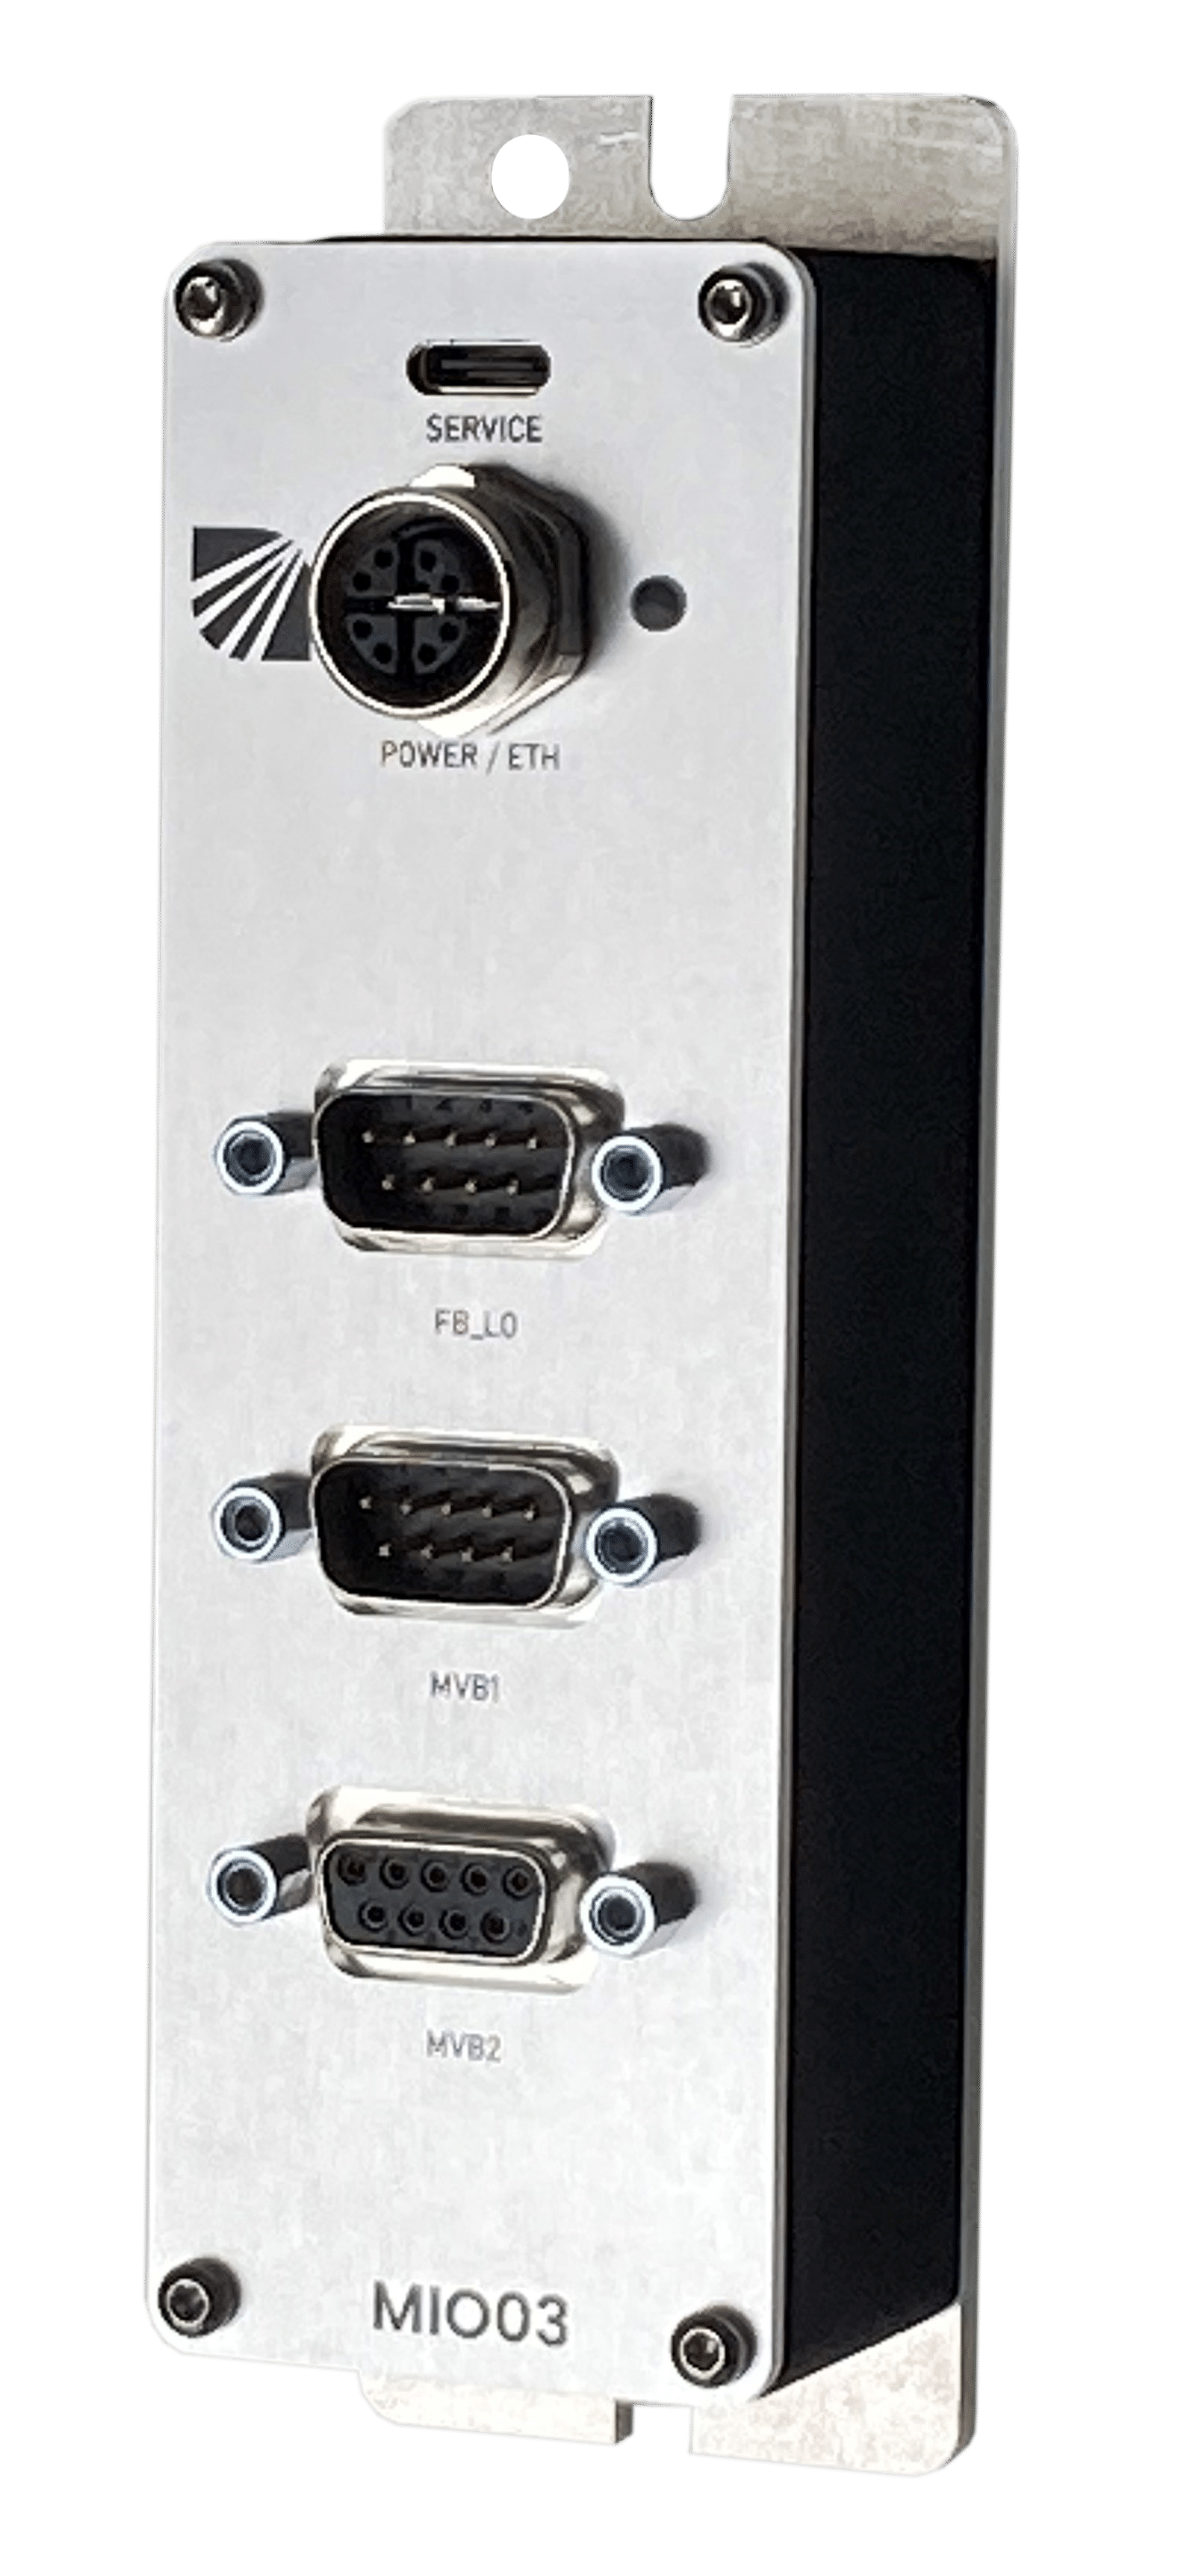
\includegraphics[width=0.7\linewidth]{Figures/Chap3/Konkurenz/CI4Rail.png}
  \captionof{figure}{\mbox{Ci4Rail Sniffer \cite{Ci4Rail}}}
  \label{fig:Ci4RailSniffer}
\end{minipage}
\hfill
\begin{minipage}{0.57\textwidth}
  \begin{tabular}{|m{3cm}|m{4.5cm}|}
   \hline
   \multicolumn{2}{|c|}{\textbf{Ci4Rail ModuSio MIO03 MVB/CAN Sniffer}} \\ \hline
    \textbf{Firma} & Ci4Rail \\ \hline
    \textbf{Datenbus} & MVB (EMD/ESD Kapitel \ref{Übertragungsmedien}), CAN \\ \hline
    \textbf{Datenraten} & MVB: 1,5 Mbps / CAN: bis zu 1 Mbps / Ethernet: 10/100 Mbps \\ \hline
    \textbf{Galvanische \mbox{Trennung}} & 750V DC (MVB/CAN/Shield) \\ \hline
    \textbf{Schnittstellen} & MVB: D-Sub 9 Pol, CAN: D-Sub 9 Pol , Ethernet: M12, Service: USB-C, WLAN: IEEE 802.11b/g/n  \\ \hline
    \textbf{Stromversorgung} & PoE oder 12/24 V DC \\ \hline
    \textbf{Einsatztemperatur} & -40 °C bis 70 °C \\ \hline
    \textbf{Schutzart} & keine Angabe \\ \hline
    \textbf{Gewicht} & keine Angabe \\ \hline
    \textbf{Abmessungen} & 151 × 42 × 51 mm \\ \hline
    \textbf{Software} &  Open Source APIs für SW-Integration \\ \hline
    \textbf{Besonderheiten} & WLAN-Firmwareupdates, CAN-Sniffer \\ \hline
  \end{tabular}
%\textcolor{red}{IP\ Based\ Sniffer}

\end{minipage}
%\newpage
%\textbf{Sniffer 3: Yacer MVB Protocol Analyzer}\\[2ex]
\begin{minipage}{0.4\textwidth}
  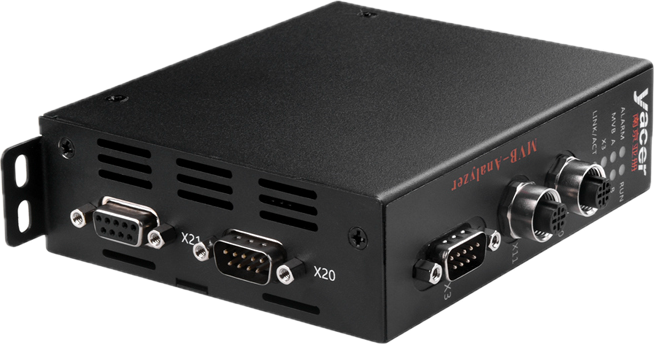
\includegraphics[width=1\linewidth]{Figures/Chap3/Konkurenz/Yacer.png}
  \captionof{figure}{MVB Protocol Analyzer \cite{Yacer}}
  \label{fig:YacerAnalyzer}
\end{minipage}
\hfill
\begin{minipage}{0.57\textwidth}
  \begin{tabular}{|m{3cm}|m{4.5cm}|}
    \hline
    \multicolumn{2}{|c|}{\textbf{Yacer MVB Protocol Analyzer}} \\ \hline
    \textbf{Firma} & Yacer \\ \hline
    \textbf{Datenbus} & MVB (EMD/ESD Kapitel \ref{Übertragungsmedien}), CAN \\ \hline
    \textbf{Datenraten} & MVB: 1,5 Mbps / CAN: bis zu 1 Mbps / Ethernet: 10/100 Mbps \\ \hline
    \textbf{Galvanische \mbox{Trennung}} & keine Angabe \\ \hline
    \textbf{Schnittstellen} & MVB: D-Sub 9 Pol, CAN: D-Sub 9 Pol , Ethernet: M12 \\ \hline
    \textbf{Stromversorgung} & 9–36 V DC (LV), 18–75 V DC (MV), \\ 
                                & 40–160 V DC (HV) \\ \hline
    \textbf{Einsatztemperatur} & -40 °C bis 70 °C \\ \hline
    \textbf{Schutzart} & keine Angabe \\ \hline
    \textbf{Gewicht} & 500 g \\ \hline
    \textbf{Abmessungen} & 124 × 36 × 104 mm \\ \hline
    \textbf{Software} & MVB-Monitor-Software \\ \hline
    \textbf{Besonderheiten} & Redundantes MVB Interface (A und B Kapitel \ref{Übertragungsmedien}), CAN-Sniffer \\ \hline
  \end{tabular}
\end{minipage}

Die Datenblätter von den Herstellern sind im Anhang \ref{app:File13}, \ref{app:File14} und \ref{app:File14} abgelegt.
%-----------------------------------
% SUBSECTION "Abgrenzung"
%-----------------------------------


\subsection{Angrenzung zu den bestehenden Produkten}

Der vorgestellte MVB-Sniffer weist im Vergleich zu bestehenden Produkten wie dem Yacer MVB-Analyzer, dem Ci4Rail MIO03 MVB/CAN Sniffer und dem AMiT MVB Analyzer mehrere technische und funktionale Unterschiede auf. Ein zentraler Unterschied liegt in der Integration von BLE (Bluetooth Low Energy), die eine kabellose Datenübertragung ermöglicht und somit die Verbindung zu mobilen Geräten oder PCs vereinfacht. Dadurch kann der Sniffer einfach mit mobilen Geräten oder PC verbunden werden, was eine zusätzliche Verkabelung überflüssig macht und die Handhabung erleichtert.

Ein weiterer Unterschied liegt in der Datenfilterung, die eine Selektion relevanter MVB-Daten gewährleistet. Dies reduziert die zu analysierende Datenmenge und kann die Effizienz bei der Fehlersuche und Diagnose in Netzwerken mit hohem Datenverkehr verbessern.

Auch in Bezug auf die Bedienung gibt es Unterschiede. Im Gegensatz zu einigen Konkurrenzprodukten soll der MVB-Sniffer ohne zusätzliche Software auskommen. In Zukunft soll der Sniffer über eine Web App konfiguriert werden können sowie Daten Visualisiert werden können

Im Bereich der Hardware soll der Sniffer durch seine kompakte Bauweise und sein geringes Gewicht in Zukunft hervorstechen. Diese Eigenschaften könnten die Mobilität und den Transport erleichtern. Ein integrierter Akku ermöglicht zudem den Einsatz des Sniffers in Situationen, in denen keine externe Stromversorgung verfügbar oder in der Nähe ist.

Zusammenfassend weist der MVB-Sniffer im Vergleich zu bestehenden Lösungen wie dem Yacer MVB-Analyzer, dem Ci4Rail MIO03 und dem AMiT MVB Analyzer Besonderheiten wie die BLE-Funktion, eine einfache Bedienbarkeit, den Verzicht auf Zusatzsoftware, einen integrierten Akku sowie eine kompakte Bauweise auf.
% !TEX root = ../main.tex

% Indicate the main file. Must go at the beginning of the file.

%-------------------------------------------------------------------------------
% CHAPTER TEMPLATE
%-------------------------------------------------------------------------------


\chapter{Theoretische Grundlagen} % Main chapter title
\label{Chapter2TheoretischeGrundlagen} % Change X to a consecutive number; for referencing this chapter elsewhere, use \ref{ChapterX}
Der MVB ist ein in der Bahnindustrie verbreiteter Fahrzeugbus, welcher auf dem Prinzip \textit{single master - multiple slaves} aufbaut. In folgenden Abschnitten werden die Grundlagen des Busses aufgezeigt. Alle Daten und Abbildungen in folgendem Kapitel wurden, wenn nicht anders deklariert, aus der Norm IEC 61375-3-1 entnommen. \cite{MVB_Norm} 

%--------------------------------------------------------------------------------
% SECTION "Multifunction Vehicle Bus"
%--------------------------------------------------------------------------------

\section{Multifunction Vehicle Bus}

%\textcolor{red}{Einführung in Grundbegriffe und das Konzept MVB, In der Regel ist zumindest ein kurzes Theoriekapitel notwendig. Es nimmt Bezug  auf das thematische Oberthema, aber natürlich nicht auf allgemeine theoretische Grundlagen etwa aus der Naturwissenschaft.}
%\textcolor{red}{Vlt noch ergänzen optisch und elektrische(EMD, ESD)Ausführungen und bei Sicherheitskritischen Anwendungen (nicht Komfort) meist Redundant geführt Linie A und B..}

Der Abschnitt beleuchtet die wesentlichen Aspekte des Physical und Link Layers des Datenbusses gemäss der Norm SN EN 61375. Der Fokus liegt auf der Datenübertragungsgeschwindigkeit, dem Bit-Encoding und den Steuermechanismen wie den Start-Delimitern und dem Master-Slave-Prinzip. Neben den technischen Grundlagen, wie der Manchester-Kodierung und den Non-Data-Symbolen, wird die Struktur von Frames und Telegrammen detailliert beschrieben.

Nachfolgende Texte sowie Illustrationen sind alle aus der Norm SN EN 61375-3-1 Kapitel 


%-----------------------------------
% SUBSECTION "MVB Bus"
%-----------------------------------

%\textcolor{red}{MVB Aufbau, Master Slave Prinzip, Telegrammme, F-Codes}
\subsection{Linklayer - Master-Frame}
\label{sub:MasterFrame}
Das Master-Frame ist der Anfang eines Telegrammes und wird immer vom Busmaster gesendet. Nach dem Startbit folgen 8 Bit, welche dem Master-Frame Delimiter in Abbildung \ref{fig:FrameDelimiterMasterSlave} entsprechen. 

\begin{figure}[H]
    \centering
    \begin{minipage}{0.33 \textwidth}
        \centering
        \begin{enumerate}
            \item Master Start-Delimiter
            \item 16 Bit Frame Data
            \begin{enumerate}
                \item F-Code: 4 Bit
                \item Data: 12 Bit
            \end{enumerate}
            \item 8 Bit check sequenze 
            \item End-Delimiter
        \end{enumerate}
    \end{minipage}
    \hfill
    \begin{minipage}{0.65 \textwidth}
        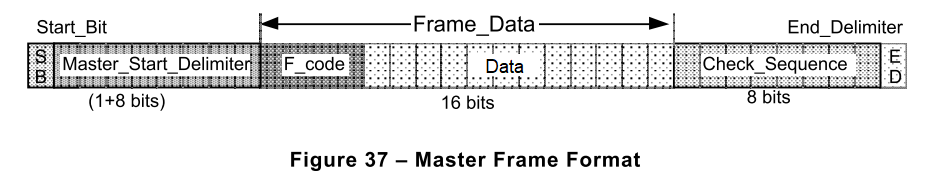
\includegraphics[width = \textwidth]{Figures/Chap2/Grundlagen/MVB_DOKU/Frames und Telegramme/Fig37_MasterFrameFormat.png}
        \caption{Master-Frame Format}
        \label{fig:MasterFrameFormat}
    \end{minipage}
        
\end{figure}

\subsection{Linkayer - Slave-Frame}
\label{sub:SlaveFrame}
Das Slave-Frame folgt direkt nach dem Master-Frame, sofern der angesprochene Slave eingeschalten und sendefähig ist. Ansonsten würde der Master nach einer definierten maximalen Wartezeit ein neues Telegramm beginnen. \newline
Im Gegensatz zum Master-Frame hat der Slave-Frame verschiedene Längen, je nach F-Code. Je nach Grösse werden ebenfalls mehrere Check-Sequenzen geschickt. Eine Check-Sequenz kann dabei bis zu 64 Bit verifizieren.

\begin{enumerate}
    \item Slave Start-Delimiter (8 Bit)
    \item 16 - 256 Bit Frame Data (individuell)
    \item Check sequence nach maximal 64 Bit Daten 
    \item End-Delimiter
\end{enumerate}

\begin{figure}[H]
    \centering
    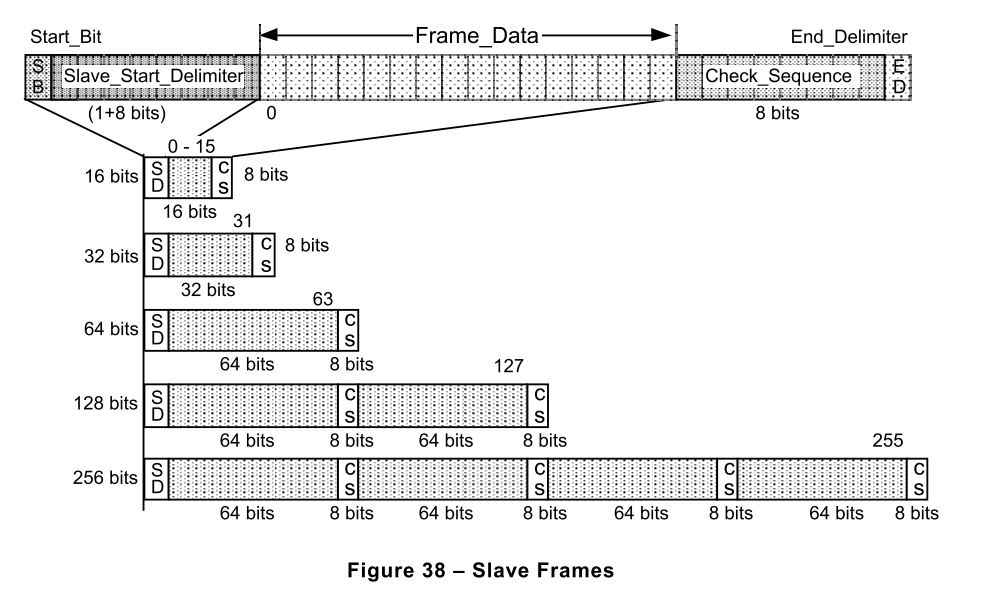
\includegraphics[width = 0.8 \textwidth]{Figures/Chap2/Grundlagen/MVB_DOKU/Frames und Telegramme/Fig38_SlaveFrameFormat.png}
    \caption{Slave-Frame Format}
    \label{fig:SlaveFrameFormat}
\end{figure}

\subsection{Linklayer - Check Sequence}
\label{sub:CheckSequenz}
Die Prüfsequenz wird als zyklische Redundanzprüfung (CRC) für die 16, 32 oder 64 Bit an Daten berechnet, welche gemäss dem generativen Polynom in Gleichung \ref{equ:GenerativesPolynom} berechnet werden soll.

\begin{equation}
    G(x) = x^7 + x^6 + x^5 + x^2 + 1
    \label{equ:GenerativesPolynom}
\end{equation}

\subsection{Link Layer - Master / Slave Prinzip}
\label{sub:MasterSlavePrinzip}
Der MVB wird mit ein Master - Slave Prinzip realisiert. Der Master fordert mit einem definierten \textit{Master\_Frame} (Kapitel \ref{sub:MasterFrame}) die Daten der jeweiligen Slave-Teilnehmer an. Der Slave beantwortet die Anfrage mit einem \textit{Slave\_Frame} (Kapitel \ref{sub:SlaveFrame}. Das Master- und Slave-Frame bilden zusammen ein Telegram (Siehe Abbildung \ref{fig:Fig39_Telegamm_definition.png}). 

\begin{figure}[H]
    \centering
    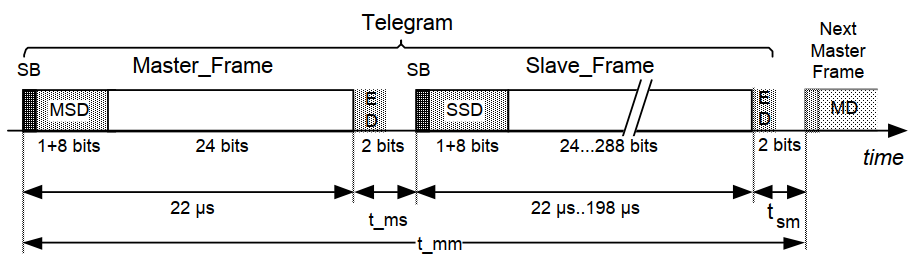
\includegraphics[width=0.85\linewidth]{Figures/Chap2/Grundlagen/MVB_DOKU/Frames und Telegramme/Fig39_Telegamm_definition.png}
    \caption{Master- und Slave-Frame bilden ein Telegram}
    \label{fig:Fig39_Telegamm_definition.png}
\end{figure}

In der Norm \textit{SN EN 61375} sind die Telegramme in 16 verschiedene Frame-Codes (F-Codes) unterteilt. In Abbildung \ref{fig:FCodeListe} ist eine tabellarische Auflistung zu sehen. 

\begin{figure}[H]
    \centering
    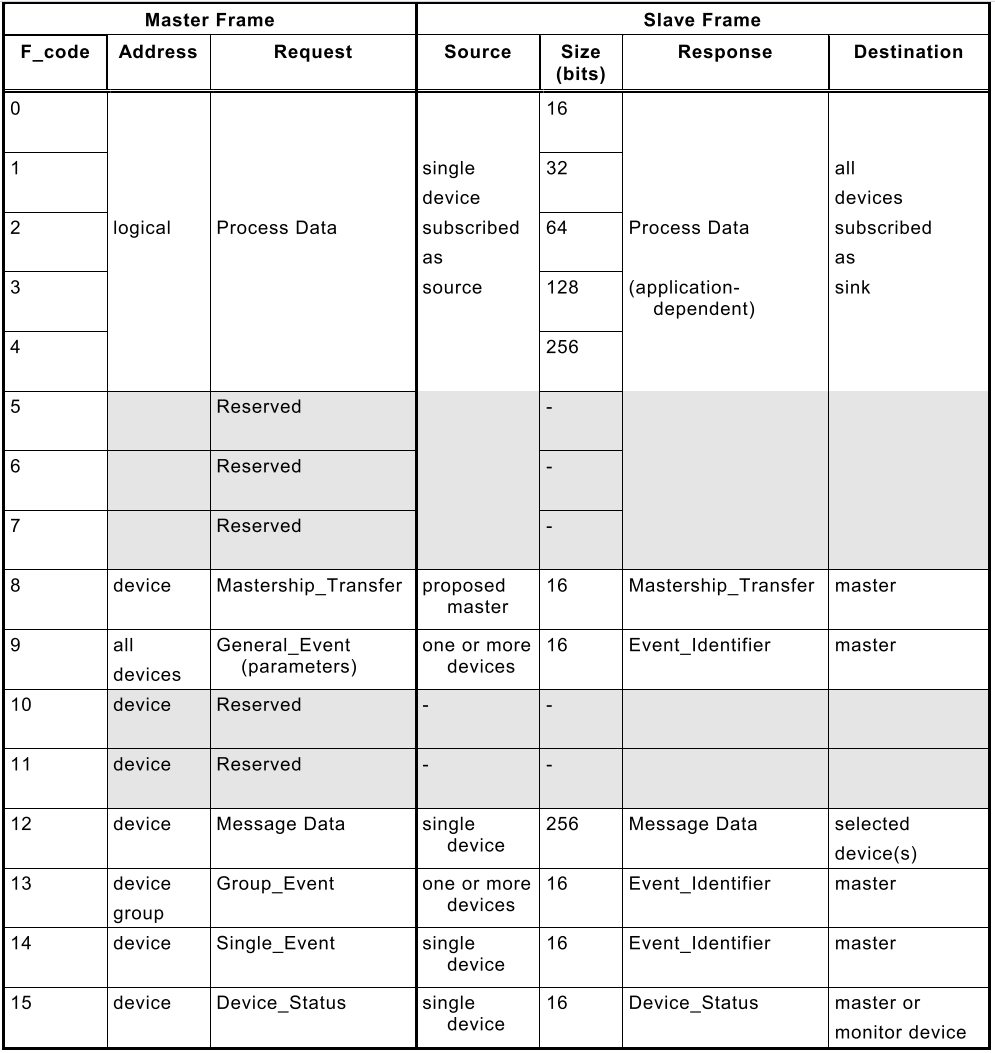
\includegraphics[width=0.9\linewidth]{Figures/Chap2/Grundlagen/MVB_DOKU/Frames und Telegramme/F-Code Liste.png}
    \caption{Auflistung aller möglichen F-Codes}
    \label{fig:FCodeListe}
\end{figure}

\subsection{Physical Layer - Geschwindigkeit auf dem Datenbus}
\label{sub:GeschwindigkeitDatenbus}
Die Signalgeschwindigkeit ist in der Norm \textit{SN EN 61375-3-1:2012 Kap. 4.3.1} definiert. Diese lautet 1.5 MBit/s $\pm$ 0.01\% mit Manchester Encoding (siehe \ref{sub:BitEncoding})

\begin{itemize}
  \item BR (Bitrate): 1.5 MHz oder 1.5 MBit/s
  \item BT (Bittime): 666.7 ns
\end{itemize}

\subsection{Physical Layer - Bit-Encoding}
\label{sub:BitEncoding}
Die Frame-Data sollen gemäss folgender \textit{Bit-Encoding} (Abb. \ref{fig:manchester_Bit_Encoding}) kodiert werden.

\begin{itemize}
    \item Eine "'1"' soll kodiert werden als ein \textbf{HIGH} in der ersten und dann ein \textbf{LOW} in der zweiten Hälfte des Bit
    \item Eine "'0"' soll kodiert werden als ein \textbf{LOW} in der ersten und dann ein \textbf{HIGH} in der zweiten Hälfte des Bit
\end{itemize}

\begin{figure}[H]
    \centering
    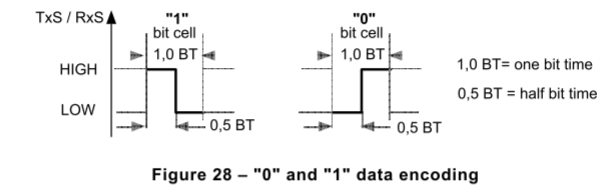
\includegraphics[width = 0.7 \textwidth]{Figures/Chap2/Grundlagen/MVB_DOKU/Layer/Bit_Encoding.png}
    \caption{Machester Bit-Encoding}
    \label{fig:manchester_Bit_Encoding}
\end{figure}

\subsection{Physical Layer - Non Data Symbols} 
\label{sub:NonDataSymbols}
Der Start-Delimiter enthält \textit{Non Data Symbols}, welche zur Synchronisierung verwendet werden. Diese Symbols werden ebenfalls \textit{Manchastercode violations} genannt. Folgende Liste zeigt, wie die Symbols (Abb. \ref{fig:NonDataSymbolsEncoding}) kodiert sind

\begin{itemize}
    \item "'NH"' soll kodiert werden als ein \textbf{HIGH} Signal während eines Bit 
    \item "'NL"' soll kodiert werden als ein \textbf{LOW} Signal während eines Bit
\end{itemize}

\begin{figure}[H]
    \centering
    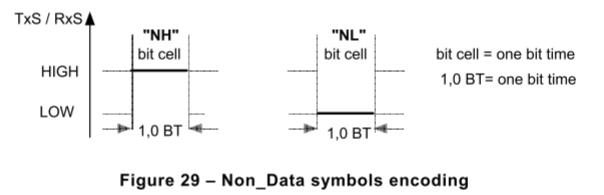
\includegraphics[width = 0.7 \textwidth]{Figures/Chap2/Grundlagen/MVB_DOKU/Layer/Non_Data_Symbol.png}
    \caption{Non Data Symbols encoding}
    \label{fig:NonDataSymbolsEncoding}
\end{figure}

\subsection{Physical Layer - Start-Delimiter}
\label{sub:StartDelimiter}
Der Start-Delimiter hat die Funktion ein Frame eindeutig zu identifizieren. Hierbei gibt es zwei unterscheidbare Start-Delimiter, der \textit{Master-Frame Delimiter} und der \textit{Slave-Frame Delimiter}. In Abbildung \ref{fig:FrameDelimiterMasterSlave} sind beide Start-Delimiter aufgezeigt. Diese Abbildung stammt aus der MVB Case Study der EPFS und ist in Anhang \ref{app:File11} auf Seite 29 zu finden. Gut zu sehen sind die in Kapitel \ref{sub:NonDataSymbols} erwähnten Manchester Violations beim Master-Frame Delimiter an Stelle 1, 2, 4 und 5 und beim Slave-Frame Delimiter an den Stellen 4, 5, 7 und 8. Das gelb markierte \textit{Start Bit} ander der Stelle 0 hat die Funktion den Start nach einer unbestimmten Zeit im Zustand \textit{Idle} zu signalisieren. Dies gehört nicht zum Start-Delimiter (siehe Abbildung \ref{fig:MasterFrameFormat} und \ref{fig:SlaveFrameFormat}). Die Manchester decodierten Start-Delimiter sind somit wie folgt aufgebaut:

\begin{itemize}
    \item Master-Frame Delimiter: [NH, NL, 0, NH, NL, 0, 0, 0]
    \item Slave-Frame Delimiter: [1, 1, 1, NL, NH, 1, NL, NH]
\end{itemize}


\begin{figure}[H]
    \centering
    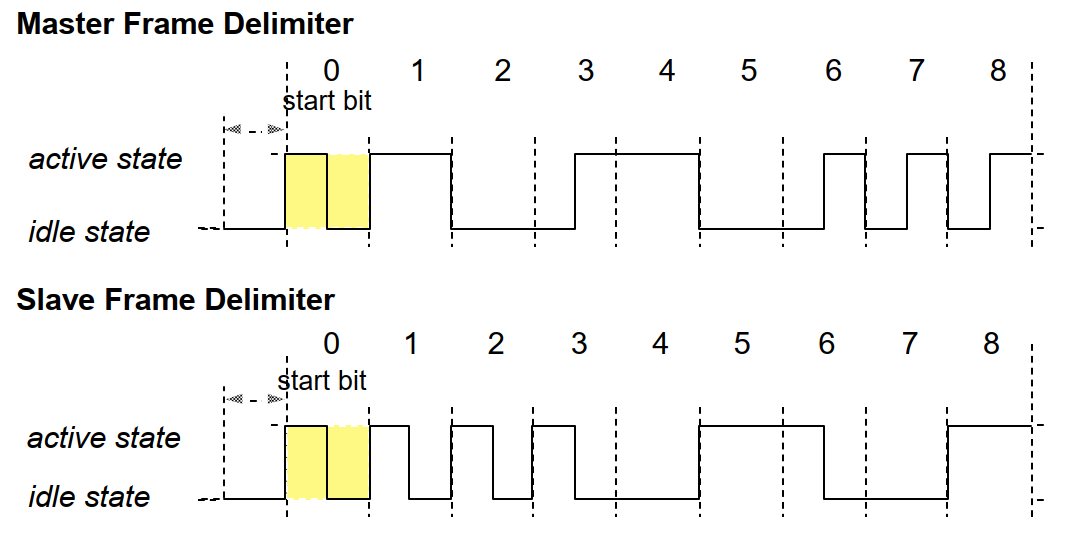
\includegraphics[width=0.8\linewidth]{Figures/Chap2/Grundlagen/MVB_DOKU/Layer/Frame_Delimiter.png}
    \caption{Illustration Master- und Slave-Frame Delimiter}
    \label{fig:FrameDelimiterMasterSlave}
\end{figure}

\section{Übertragungsmedien}
\label{Übertragungsmedien}

Für den MVB sind in der Norm \textit{SN EN 61375-3-1 Kapitel 4.4 bis 4.6 } drei Varianten definiert. Diese sind wie folgt:
\begin{itemize}
    \item \textbf{ESD:} Electrical Short Distance Bus
    Über eine Signalleitung mit Potenzialtrennung mit Optokoppler oder ohne Potenzialtrennung
    \item  \textbf{EMD:} Electrical Middle Distance Bus
    Über verdrillte Signalleitung und Potenzialtrennung über Induktivität
    \item  \textbf{OGF:} Optical Glass Fiber
    Über ein Lichtwellenleiter
\end{itemize}

In Abbildung \ref{fig:TransceiverInterface} ist eine Illustration der drei Übertragungsmedien gezeigt. 

\begin{figure}[H]
    \centering
    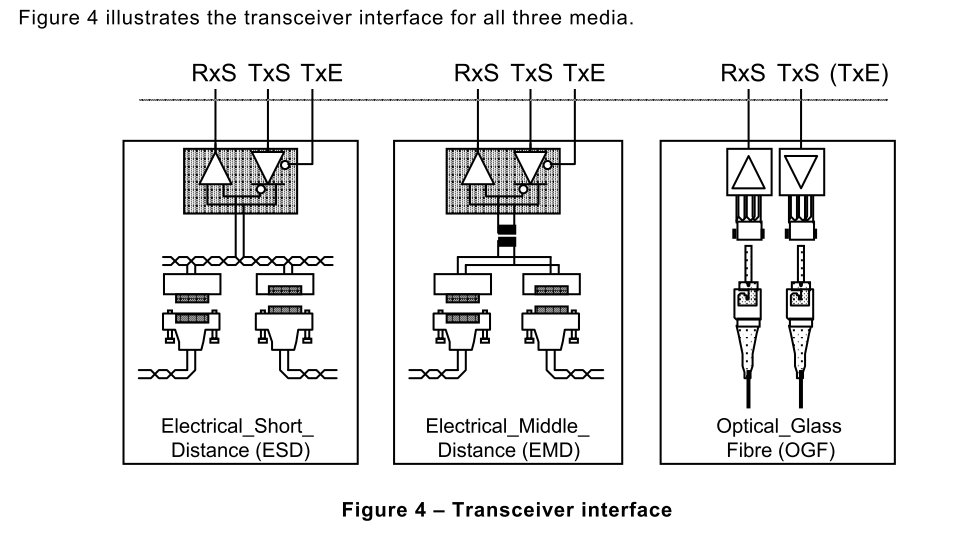
\includegraphics[width=0.9\linewidth]{Figures/Chap2/Grundlagen/MVB_DOKU/EMD_ESD_OGF/Fig4_Transceiver interface.png}
    \caption{Transceiver Interfaces}
    \label{fig:TransceiverInterface}
\end{figure}

Die Verbindungen zwischen ESD und EMD erfolgen über einen D-Sub9-Stecker. Tabelle \ref{tab:PinESDEMD} zeigt die Pinbelegung der Stecker sowie deren Funktionen. Dabei wird zwischen \textit{A Bus} und \textit{B Bus} unterschieden, da der MVB redundant geführt ist und auf den jeweiligen Leitungen A und B gespiegelt wird. Die Details zur Redundanz werden nicht weiter behandelt.


\begin{table}[H]
    \centering
    \begin{tabular}{|r||c|c|} \hline
        Pin & ESD & EMD\\ \hline
        1 & A Data Positiv & A Data Positiv\\ \hline
        2 & A Data Negativ & A Data Negativ\\ \hline
        3 & TxE (optional) & TxE (optional)\\ \hline
        4 & B Data Positiv & B Data Positiv\\ \hline
        5 & B Data Negativ & B Data Negativ\\ \hline
        6 & A Bus Ground & A Positiv Pole\\ \hline
        7 & B Bus Ground & A Negativ Pole\\ \hline
        8 & A Bus 5V & B Positiv Pole\\ \hline
        9 & B Bus 5V & B Negativ Pole\\ \hline
    \end{tabular}
    \caption{Pinbelegung für ESD und EMD Stecker}
    \label{tab:PinESDEMD}
\end{table}

Für das Übertragungsmedium OGF ist keine Pinbelegung erforderlich, da zwei separate Lichtwellenleiter verwendet werden: Einer dient zum Senden, der andere zum Empfangen von Signalen.
%\include{Chapters/Kapitel3.1_Recherche}
\chapter{Methode} % Main chapter title
\label{chapter3:Methode} % Change X to a consecutive number; for referencing this chapter elsewhere, use \ref{ChapterX}

\section{Design eigener Sniffer}
\label{Design Sniffer}

Zu Beginn der Projektarbeit wurde ein Prozessdiagramm erstellt, welches aufzeigen soll, welche Hardware
benötigt wird um einen Sniffer entwickeln zu können, welcher vom MVB lesen kann.
Dieser erste Entwurf ist in Abbildung \ref{fig:AufbauSnifferDraft} zu sehen.

\begin{figure}[H]
    \centering
    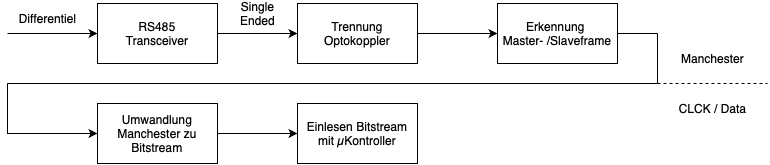
\includegraphics[width=1\linewidth]{Figures/Chap3/Design Eigener Sniffer/Sniffer_Aufbau_Draft.png}
    \caption{Erste Darstellung Aufbau Sniffer}
    \label{fig:AufbauSnifferDraft}
\end{figure}

Der Entwurf diente als Grundlage auf welcher aufgebaut werden konnte. Aus dem Entwurf entstand dann
ein ausführlicher schematischer Aufbau, in dem auch gleich die Anforderungen zum Sniffer aufgeführt
sind. 

Dieser Aufbau, wie er in Abbildung \ref{fig:AufbauSniffer} zu sehen ist, zeigt die verwendete Hardware
auf und wie diese untereinander verbunden sind.

\begin{figure}[H]
    \centering
    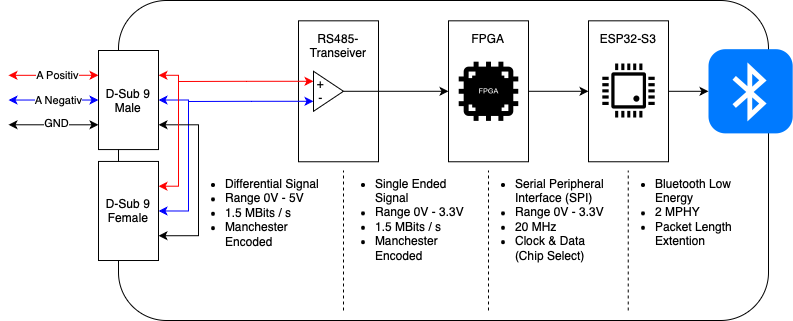
\includegraphics[width=0.9\linewidth]{Figures/Chap3/Design Eigener Sniffer/Aufbau_Sniffer.png}
    \caption{Schematischer Aufbau Sniffer}
    \label{fig:AufbauSniffer}
\end{figure}


Es ist zu sehen dass vom ersten zum finalen Aufbau, der Baustein "'\textit{Trennung Optokoppler}"'
wegfällt, da durch den RS485-Transceiver sichergestellt wird, dass der Bus nie beschrieben werden kann.
Im finalen Design kommt zusätzlich die Ausgabe über Bluetooth hinzu welche zu beginn nicht angedacht
war.

Um aus dem Differentiellen Manchestersignal vom MVB ein Single-Ended Signal, welches "'0 V"' bei einer 
Negativen Flanke und "'3.3 V"' bei einer Positiven Flanke annehmen soll, erzeugen zu können, wurde ein
RS485-Transceiver verwendet. Der Transceiver wird mit einer Spannung von "'3.3 V"' versorgt. Das
erzeugte digitale Signal vom RS485 wird weiter ins FPGA (Field Programmable Gate Array) geleitet, wo
der Manchestercode decodiert wird und als Bitstream über das SPI an den µKontroller ESP32 gesendet
wird. Der µKontroller wertet die Daten aus und gibt dann die entsprechenden Codes per Bluetooth aus.

In einer Prototypenphase und somit auch im Rahmen der Projektarbeit, sind dafür drei verschiedene
Evaluationsboards verwendet worden. Das definierte Ziel für den fertigen Sniffer, welches in der
Bachelorarbeit angestrebt wird, ist es ein eigenes PCB zu erstellen, welche die benötigten Bauteile auf
einem Board vereint. Ebenfalls soll der fertige Sniffer ein schützendes und abschliessendes Gehäuse,
mit den nötigen Ausschnitten besitzen.

\subsection{Wahl der Hardware}
In den folgenden Kapitel wird erläutert warum die entsprechende Hardware für den MVB-Sniffer gewählt
wurde. In den Kapitel \ref{chapter5:Diskussion} und \ref{chapter6:Ausblick} werden die Wahl der
Hardware nochmals abschliessend diskutiert und, allfällige Änderungen in der Wahl, als Ausblick 
festgehalten.


\subsubsection{RS485}
Der RS485 Transceiver macht aus einem differentiellen Signal ein Digitales Signal, welches zwischen der Speisespannung und 0V hin und her wechselt. Das Ausgangssignal kann dann im Falle des MVB von Busteilnehmern ausgewertet werden. Da im Anwendungsbereich des MVB (ESD) auf den Schienenfahrzeugen, für welche der Sniffer ausgelegt wird, bereits RS485 Transceiver eingesetzt werden, war es naheliegend und sinnvoll diese auch für den Sniffer einzusetzen.

\subsubsection{FPGA}
In einer ersten Recherche war eine Lösungsvariante, die Decodierung des Manchestersignal in einer reinen Hardwarelösung wie sie in Abbildung \ref{} zu sehen ist umzusetzen. Als eine weitere Variante wurde dann das FPGA zur Umsetzung des Decoders in Anbetracht gezogen.
Der Entscheid für den FPGA und gegen die, nicht programmierbare, reine Hardwarelogik, lag in folgenden Punkten:
\begin{itemize}
  \item Die Logik des FPGA ist flexibel und schnell anpassbar.
  \item Das FPGA kann weiter konfiguriert werden um bei einer Weiterentwicklung des Sniffers, können weitere Aufgaben Problemlos zu implementiert werden.
  \item Das Interesse ein FPGA und dessen Programmierung in VHDL näher kennen zu lernen war gross und in diesem Projekt sicherlich gut realisierbar.
\end{itemize}

\newpage
\subsubsection{SPI}
Für die Kommunikation zwischen FPGA und ESP32 wurde das Protokoll SPI gewählt, weil es diese Kommunikation möglich macht gleichzeitig zu schreiben und aber auch Daten zu empfangen, SPI ist \textit{"'Full Duplex"'}. Des weiteren können mit diesem Übertragungsprotokoll sehr hohe Raten erreicht werden, welche bei der berechneten Busauslastung (siehe Kapitel \ref{fig:MessaufbauBusauslastungMessen}) von Vorteil ist. Alternativ hätten weitere Protokolle gewählt werden können. In Tabelle \ref{tab:spi_vergleich} ist ein kurzer Vergleich von SPI und zwei alternativen Kommunikationsprotokollen I²C und UART zu sehen. SPI ist dabei, wie bereits erwähnt, mit Abstand am schnellsten und auch einfach zu implementieren.

\begin{table}[ht]
\renewcommand{\arraystretch}{1.5} % Zeilenabstand erhöhen
\centering
\begin{tabular}{@{}p{3.4cm}p{3.2cm}p{3.2cm}p{3.2cm}@{}}
\toprule
\textbf{Merkmal}        & \textbf{SPI} & \textbf{I²C} & \textbf{UART} \\ \midrule
\textbf{Kommunikationsart} & Full duplex & Half duplex & Half duplex \\
\textbf{Anzahl Leitungen} & 4 (MISO, MOSI, SCLK, SS) & 2 (SDA, SCL) & 2 (TX, RX) \\
\textbf{Taktung}        & Synchron & Synchron & Asynchron \\
\textbf{Datenrate}      & 50+ Mbit/s & Bis zu 4 Mbit/s & Bis zu 1 Mbit/s \\
\textbf{Vorteile}       & Hohe Datenrate, Full duplex, einfache Hardware & Wenige Leitungen, mehrere Geräte auf einem Bus & Einfach zu implementieren, universell einsetzbar \\
\textbf{Nachteile}      & Viele Leitungen bei mehreren Slaves, keine eingebaute Fehlerkorrektur & Geringere Geschwindigkeit, zusätzliche Protokollverwaltung & Keine Taktleitung, potenziell ungenau bei Baudrate-Mismatch \\
\bottomrule
\end{tabular}
\caption{Vergleich zwischen SPI, I²C und UART}
\label{tab:spi_vergleich}
\end{table}

\subsubsection{ESP32}
\textcolor{red}{Warum wurde der µKontroller ESP32 gewählt?}\\
Der ESP32 wurde gewählt, weil dieser die Funktionalität von Bluetooth Low Energy 


\section{Busauslastung messen}
Um zu beurteilen, ob Bluetooth Low Energy (BLE) eine geeignete Lösung für die Übertragung von Telegrammen vom Sniffer zum Endgerät darstellt, wurde die Busauslastung mittels Oszilloskop aufgezeichnet und mittels Matlab ausgewertet. Ziel war es abzuschätzen, ob die effektiven Nutzdaten über BLE übertragen werden können. Gleichzeitig sollen ersten Erfahrungen im Bereich der Signalauswertung gemacht werden, welche für die Implementierung im FPGA genutzt werden können.

Für die Analyse wurden zwei Messungen durchgeführt: Eine unter Normallast und eine unter Volllast. Die Volllast wurde simuliert indem der Depot-Diagnosespeicher (DDS) auf dem Fahrzeugdisplay abgerufen wurde. Dies führte dazu, dass der Speicher die entsprechenden Daten über den Bus an das Display sendete, was kurzfristig zu einer höheren Auslastung führte.

Die Messungen wurden mit einem Picoscope 2207B durchgeführt, während die anschliessende Auswertung mit Matlab realisiert wurde.

\subsection{Messaufbau}

Der Messaufbau ist in Abbildung \ref{fig:MessaufbauBusauslastungMessen} dargestellt. Um die Busauslastung zu messen, wurde die MVB-Leitung, die normalerweise von Gerät zu Gerät durchgeschleift ist, an einer geeigneten Stelle unterbrochen und ein Leitungsaufteiler eingefügt. Dies ermöglichte den direkten Zugriff auf die differentiellen Leitungen des Busses mit dem Picoscope. Der MVB-Loop wurde dabei wieder geschlossen, sodass keine Geräte vom Bus abgetrennt wurden. Die gemessenen Daten wurden über eine USB-Schnittstelle an einen Laptop übertragen und dort mit der Pico-Software aufgezeichnet.

\begin{figure}[H]
    \centering
    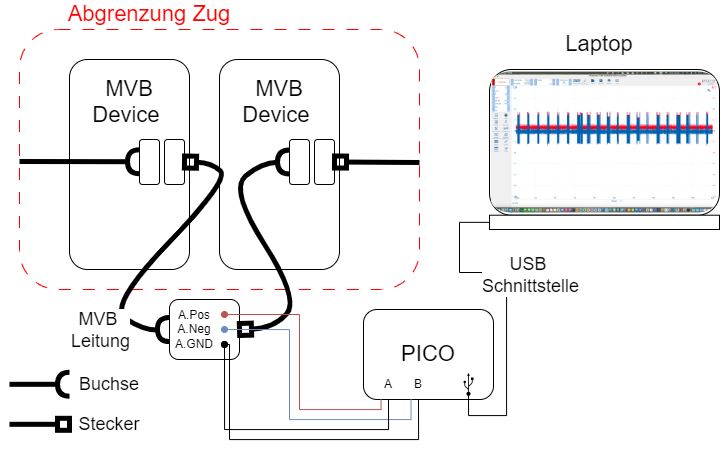
\includegraphics[width=0.8\linewidth]{Figures/Chap3/Busauslastung/Messaufbau_PICO_IC2000.png}
    \caption{Messaufbau Busauslastung messen}
    \label{fig:MessaufbauBusauslastungMessen}
\end{figure}

Die erfassten Daten wurden anschliessend in das Matlab-Dateiformat (.mat) exportiert. Die Struktur der Matlab-Datei ist in Abbildung \ref{fig:MatlabFileStruktur} dargestellt. Die Variablen \textit{A} und \textit{B} entsprechen den Messpunkten des Picoscope, während \textit{Tinterval} die Zeit zwischen zwei Messpunkten angibt. 

\begin{figure}[H]
    \centering
    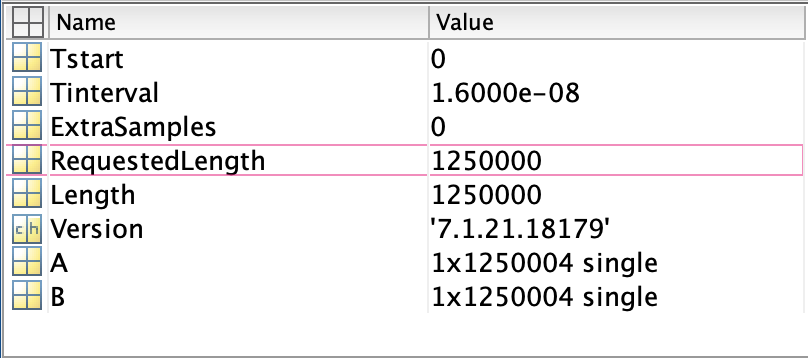
\includegraphics[width=0.5\linewidth]{Figures/Chap3/Busauslastung/Matlab_file_struktur.png}
    \caption{Matlab File Struktur}
    \label{fig:MatlabFileStruktur}
\end{figure}

Der Messaufbau blieb für die Messungen unter Normallast und Volllast identisch. Um die Volllast zu simulieren, wurde der Befehl zur Anzeige der DDS auf dem Fahrzeugdisplay ausgelöst, bevor die Messung gestartet wurde. Der Zeitraum zwischen der Eingabe des Befehls und der Darstellung der Daten auf dem Display beträgt etwa 5 Sekunden.

Das Picoscope-Oszilloskop wurde für die Messung mit einer Abtastrate von 62,5 MS/s konfiguriert, was einem Abtastintervall von 16 ns entspricht. Diese maximale Abtastrate wurde gewählt, um selbst kleinste Signaländerungen erfassen zu können. 

\subsection{Matlab Auswertung}
Die Auswertung der Analogwerte wurde mit Matlab realisiert. Ziel war es, herauszufinden, wie gross die Busauslastung in Bits/s ist. Für die Übertragung mit Bluetooth waren alle Daten ausser die Startdelimiter (siehe Kapitel \ref{sub:StartDelimiter}) von Interesse. Die Auswertung mit Matlab war ebenfalls eine Überlegungsgrundlage für die spätere Implementierung in den FPGA (siehe Kapitel \ref{Manchester Decodierung}). Die Auswertung ist in folgende Schritte untertielt:
\begin{enumerate}
    \item Delimiter Erkennung
    \item Bestimmung Anzahl Bits
    \item Differenz bilden
\end{enumerate}


\subsubsection{Delimiter erkennen}
%\textcolor{red}{Anzahl delimiter erkennen. Charakteristik erkannt -> letzte werte Idle, dann Nulldurchgang, aber nur wenn einer der nächsten 20 Werte über null ist, sonst wurde peak am schluss auch gezählt. }
Um die Startdelimiter zu erkennen, wurde die Charakteristik eines Delimiters gemäss Kapitel \ref{sub:StartDelimiter} untersucht. In Abbildung \ref{fig:AusschnittMvbOhneDds} wurde der Zeitbereich vergrössert. Dadurch lässt sich ein Telegramme (gemäss Kapitel \ref{sub:MasterSlavePrinzip}) besser sehen.

\begin{figure}[H]
    \centering
    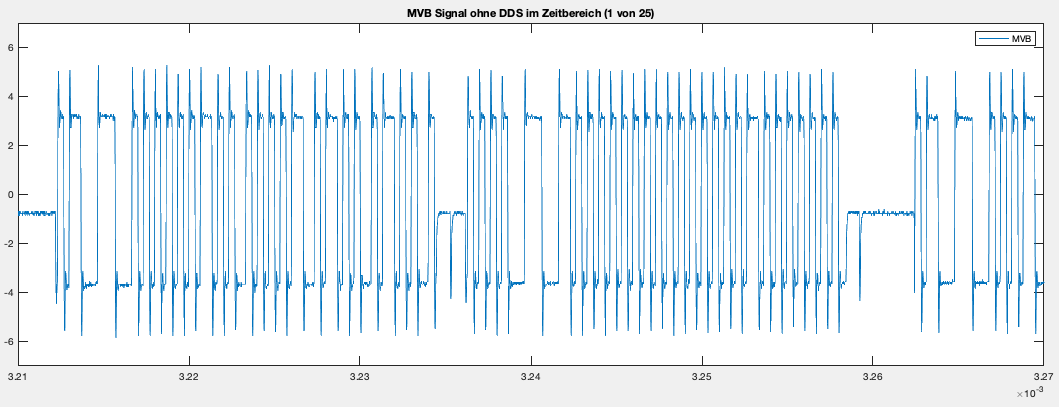
\includegraphics[width=0.8\linewidth]{Figures/Chap3/Busauslastung/Ausschnitt_MVB_ohne_Delimiter.png}
    \caption{Ausschnitt MVB Signal ohne DDS}
    \label{fig:AusschnittMvbOhneDds}
\end{figure}

Zu sehen ist, ein vollständiges Master-Frame, das darauffolgende Slave-Frame und der Anfang des nächsten Master-Frames. Das Idle Signal verbindet die Frames. Der Startdelimiter fängt bei der ersten negativen Flanke an. Gemäss Norm muss das Slave-Frame in einem Zeitraum zwischen 2 - 6 $\mu$s folgen. Somit kann die Charakteristik des Startdelimiters wie folgt zusammengefasst werden: Ist das Idle Signal für mindestens 2 μs anstehend, beginnt der Startdelimiter bei der ersten negativen Flanke

Diese Definition konnte so nicht umgesetzt werden, da dies zu mehreren Fehlererkennungen geführt hat, da die Periode zwischen Master- und Slave-Frame teilweise unter 2 $\mu$s waren und weil ein negativer Puls am Ende des Master- oder Slave-Frames die Bedingung der Idle Zeit verletzte. Stattdessen wurde ein Zeitbereich von 0.5 Bitdauer gewählt und die zusätzliche Bedingung eingeführt, dass nach Erkennung einer negativen Flanke in der nächsten 0.5 Bitdauer mindestens ein Wert über 0V sein muss. Daraus gab sich der Algorithmus zur Erkennung der Startdelimiter und die erkannten Punkte werden in Abbildung \ref{fig:enter-label} gezeigt.

\begin{figure}[H]
    \centering
    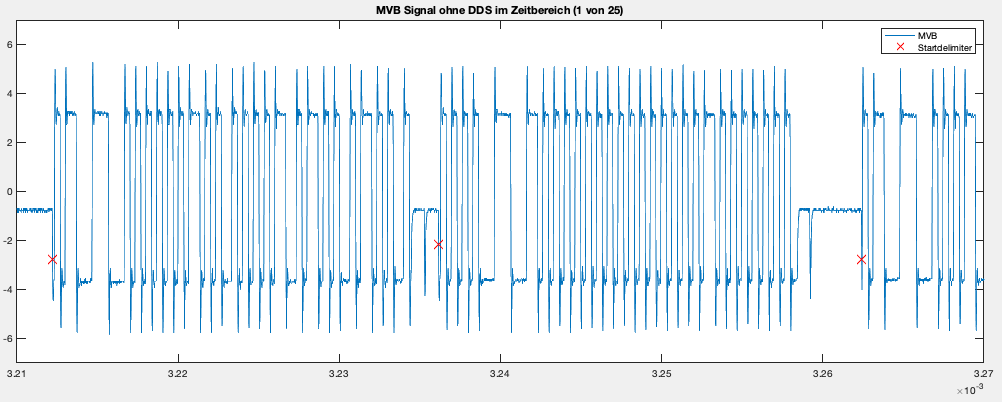
\includegraphics[width=0.8\linewidth]{Figures/Chap3/Busauslastung/Ausschnitt_MVB_mit_Delimiter.png}
    \caption{Ausschnitt der MVB Messung unter Normallast mit
Startdelimiter Erkennung (rote X)}
    \label{fig:enter-label}
\end{figure}


\subsubsection{Anzahl Bits}
\label{subsub:Nulldurchgänge}
%\textcolor{red}{Anzahl bits mit Startdelimiter erkennen. Als erstes alle werte zwischen 0 und -1V gelöscht, weil Idle. Dann wurde eine Flanke detektiert. Wenn eine Flanke detektier um 30 Werte vorwärts springen (damit zweite Flange nicht nochmals erkennt wird (manchester encodiertes Signal)}
In diesem Schritt wurde mit Matlab versucht, die Anzahl Bits zu aus der Messung auszuwerten. Gemäss Kapitel \ref{sub:BitEncoding} gibt es für den Wert "'0"' und "'1"' jeweils einen Flankenwechsel in der Hälfte der Bitdauern (BT, gemäss Kapitel \ref{sub:GeschwindigkeitDatenbus}: 1 BT = 666 ns). Dies kann verwendet werden um die Anzahl Bits herauszufinden. Anhand Abbildung \ref{fig:Suchalgo_Bits} kann der gewählte Suchalgorithmus erklärt werden.

\begin{figure}[H]
    \centering
    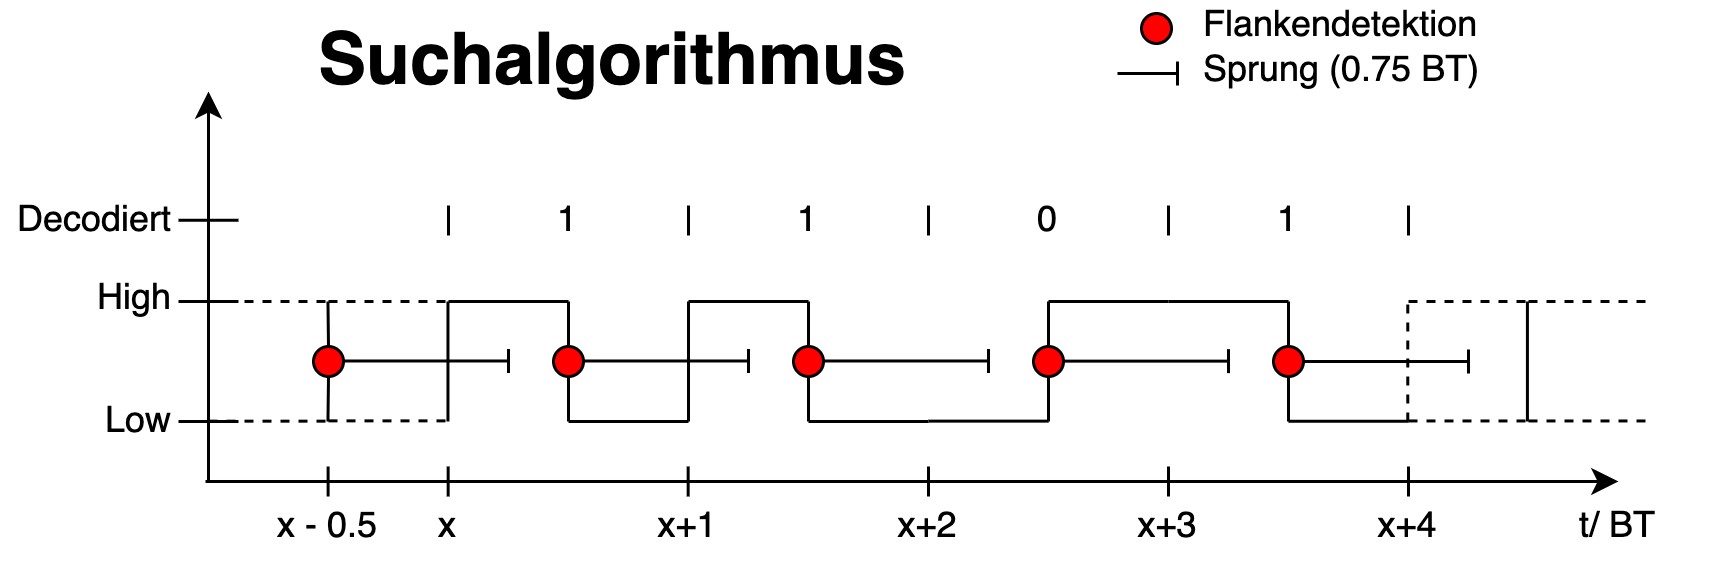
\includegraphics[width=0.9\linewidth]{Figures/Chap3/Busauslastung/Suchalgorithmus_Bits.png}
    \caption{Suchalgorithmus der Bits in einem Manchester encodierten Signal}
    \label{fig:Suchalgo_Bits}
\end{figure}

X steht für eine zufällige Zeit innerhalb einer Transaktion am Anfang eines Manchester Bits. Auf der Abszisse ist die Zeit in Bitdauer aufgetragen. Auf der Ordinate ist ein Beispielsignal und die Decodierung des Signals aufgezeigt. Da in der Mitte der Bitdauer eine Flanke zu erwarten ist, wird auch eine halbe Bitdauer vor X eine Flanke erwartet. Dies bildet den Einstieg. Wird eine Flanke detektiert, wird um eine Bitdauer von 0.75 positiv in der Zeit gesprungen. Der Sprungpfeil zeigt mit seinem flachen Ende, ab wo die nächste Flanke gesucht wird. Der Sprung erfolgt, weil Flankendetektionen wie bei \textit{x+1} in Abbildung\ref{fig:Suchalgo_Bits},  nicht berücksichtigt werden, da diese die Auswertung verfälschen.

Gemäss Anhang \ref{app:Flankenerkennung Bits} sind die Anzahl Flanken, welche in einem Master Startdelimiter und einem Slave Startdelimiter gezählt werden gleich Sieben.

Für die Auswertung am MVB Signal wurde in einem ersten Schritt das Idle Signal, also alle Messpunkte zwischen -0.5 V und -1 V aus dem Signal entfernt. Daraus folgt ein Signal,  welches Startbits, Startdelimiter, Masterframe- sowie Slaveframe-Daten enthält. In Abbildung \ref{fig:ReineDaten}ist ein Vergleich zwischen beiden Signalen zu sehen: oben mit Idle Signal, unten ohne Idle Signal. Die Idle Zeit macht somit 75 \% aus. 

\begin{figure}[H]
    \centering
    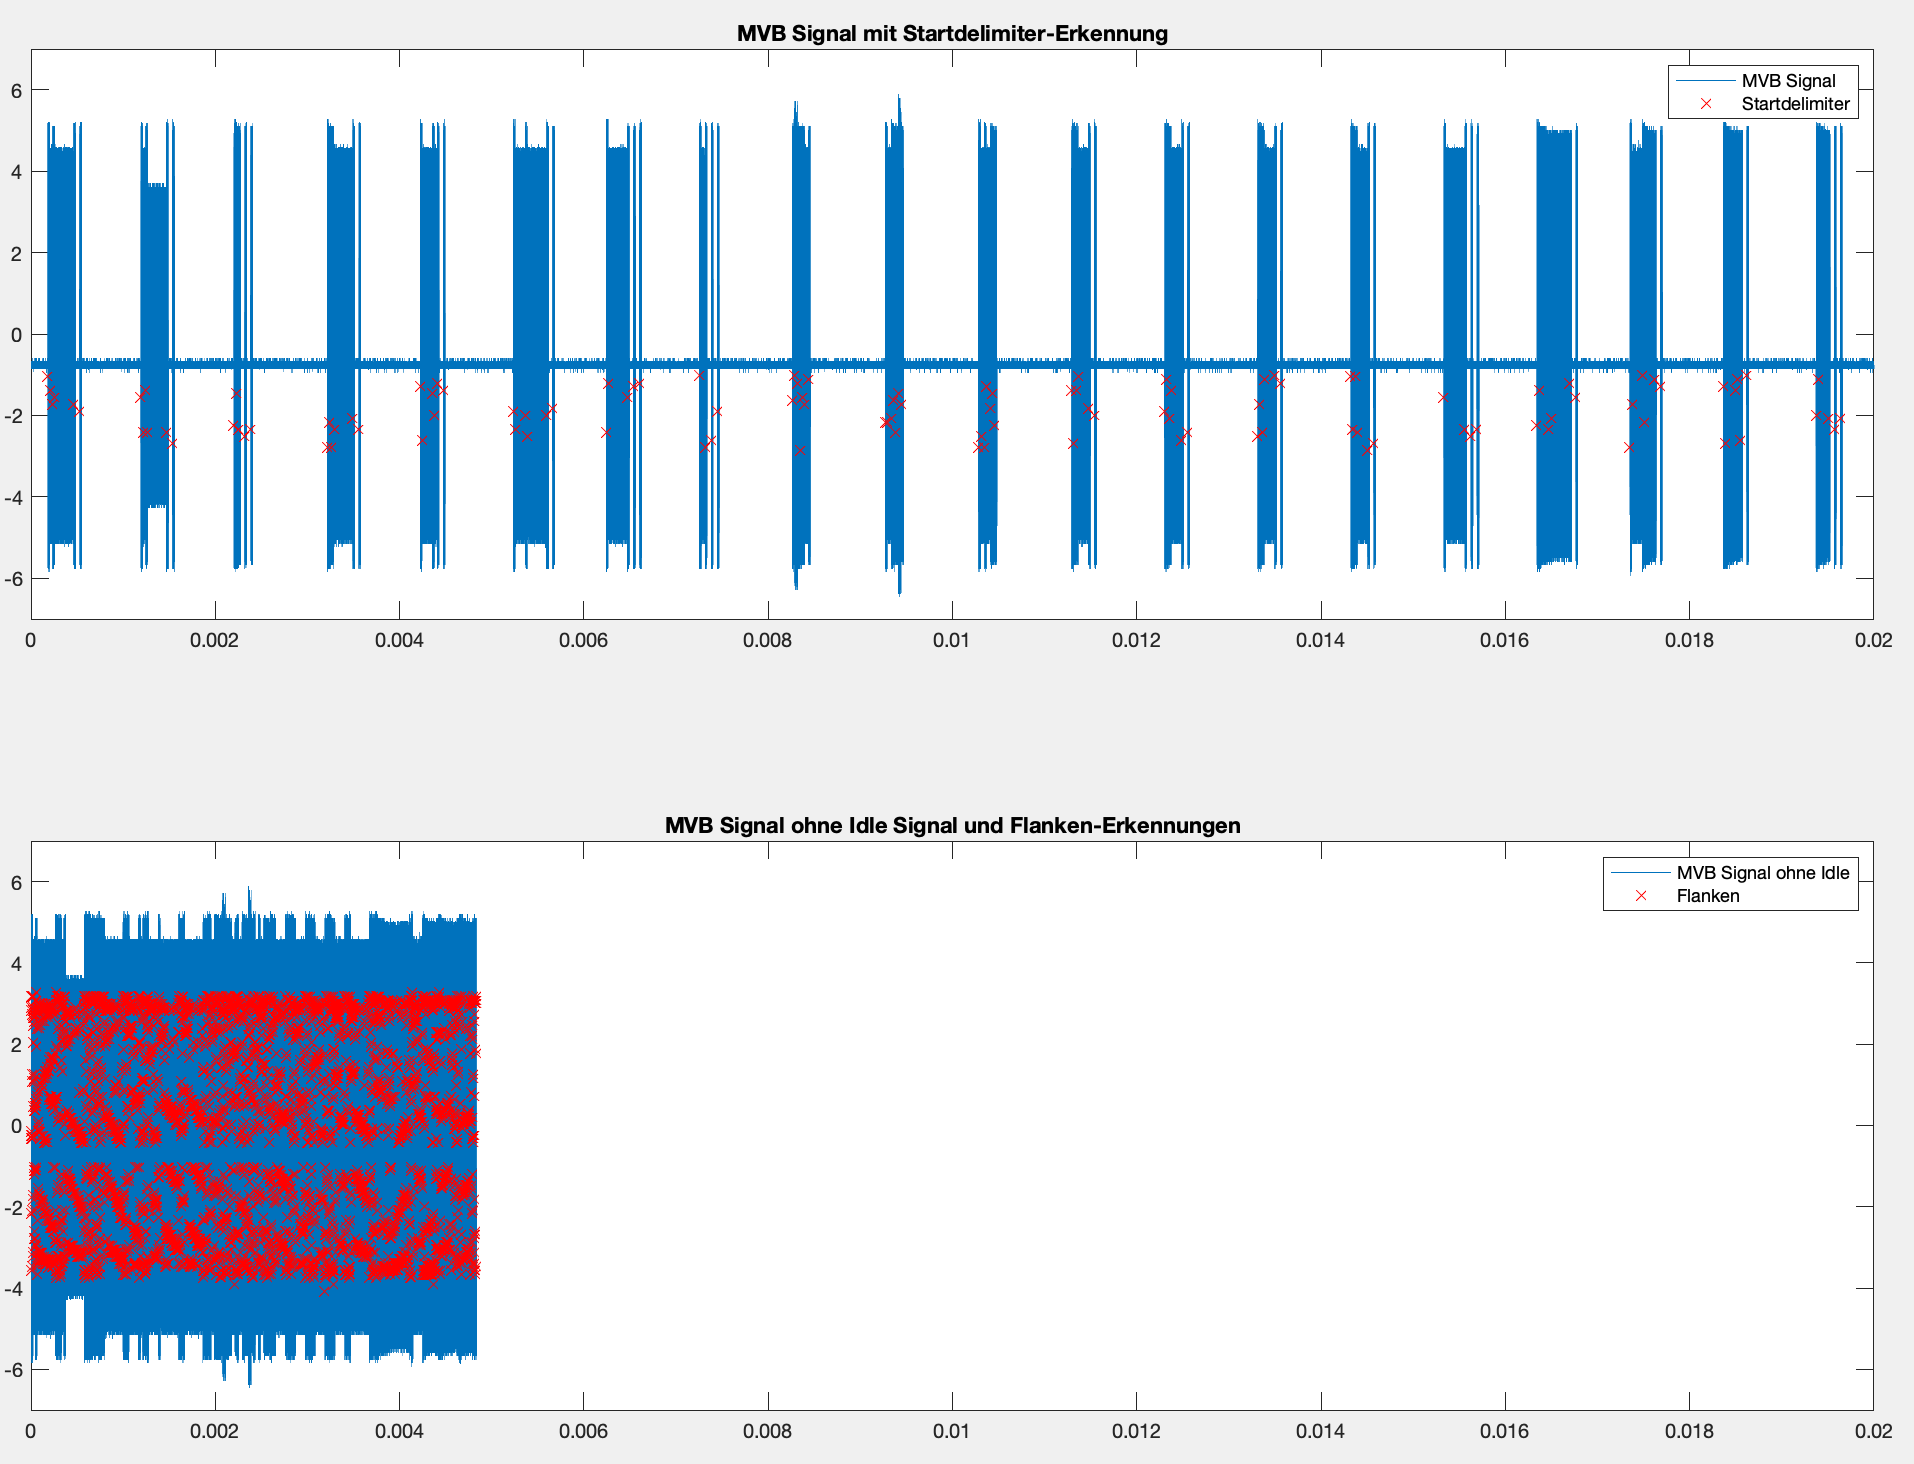
\includegraphics[width=0.75\linewidth]{Figures/Chap3/Busauslastung/Vergleich_MVB_mit_ohne_Idle.png}
    \caption{Vergleich MVB Signal mit und ohne Idle Signal (oben und unten) über einen Zeitraum von 20ms}
    \label{fig:ReineDaten}
\end{figure}

Der Suchalgorithmus wurde auf die Daten angewendet und die Anzahl Bits gezählt.

\subsubsection{Auswertung effektive Nutzdaten}
%\textcolor{red}{Effektive = Anzahl Nuldurchgänge - (Delimiert * 9); Tablle effiktive Nutzwerte mit und ohne DDS.}
Anschliessend wird ausgewertet, wie viele Bits an effektivem Payload innerhalb einer Zeitdauer von 20 ms geschickt werden. Anhand Formel \ref{equ:effektivBPS} kann dies  für jede der 25 Messungen unter Normallast und unter Volllast berechnet werden.  Der dazugehörige Code ist in Anhang \textcolor{red}{\ref{XX}} zu finden.

\begin{equation}
    eff\_bps = (NumBit - (NumDelimiter * 7)) / 0.02
    \label{equ:effektivBPS}
\end{equation}


 Die Tabelle \ref{tab:Busauslastung} zeigt die Auswertung  der Busauslastung. Die Spalten 1 und 3 enthalten die minimalen, sowie maximalen Werte der je 25 Messungen. Die Spalte \textit{mean} wurde mit dem Matlabbefehl \textit{mean()} berechnet und gibt den Mittelwert über die je 25 Messungen aus. 

\begin{table}[H]
    \centering
    \begin{tabular}{r|c|c|c}
        & min in Bits/s & mean in Bits/s & max in Bits/s\\ 
        \hline
        Normallast & 2.4705e+05 & 2.8823e+05 & 3.1885e+05\\
        \hline
        Volllast & 2.5935e+05 & 3.0456e+05 & 4.204e+05 \\
    \end{tabular}
    \caption{Busauslastung in Normallast und Volllast (ohne und mit DDS) }
    \label{tab:Busauslastung}
\end{table}

Dies bestätigt sich aus Abbildung \ref{fig:ReineDaten}, wo das Signal ohne Idle Zeit nur noch ungefähr 0.005 s lang ist. 0.005 s/0.02 s = 0.25  also 25 \% und 0.25*1.5 MBits/s sind 375 kBits/s. 

Gemäss einer Internetsuche ist es mit der Data Length Extension (DLE) und dem 2 MBits/s physikalischen Layer (PHY) möglich, bis zu 992.07 kBits/s an Datendurchsatz zu erlangen. Dies bei einem Datenaustausch von 247 Bytes. Der Wert mit der DLE und dem 1 MPHY liegt bei 400 kBits/s mit 158 Bytes an Daten. Beide Tests wurden in einem Connection Interval von 7.5 Millisekunden durchgeführt. 
Gemäss der Internetsuche sollte es also möglich sein, den vollen Rohdatenstream über Bluetooth zu senden. 



%----------------------------------------------------------------------
% SECTION Hardware FPGA

%Themen nach Signalfluss aufbauen
%----------------------------------------------------------------------

\section{Hardware FPGA}
\label{sec:HardwareFPGA}
Das FPGA soll die Umwandlung des Manchestersignals vom MVB, bzw. des Signals
nach dem RS485 Transceiver, in einen Bitstream realisieren. 

Die Konfiguration für das FPGA wurde in der Hardwarebeschreibungssprache VHDL geschrieben. Dabei wurden
mehrere Dateien für die verschiedenen Aufgaben des FPGA erstellt, um eine saubere und simple 
Dateistruktur zu erreichen. Der Code wurde mittels der Designsoftware Quartus geschrieben,
synthetisiert und auf das FPGA geladen.

Der Code ist in fünf Dateien aufgeteilt. Zwar wurde dieser in seine verschiedenen Aufgaben, der
Decodierung des Signals (siehe Kapitel \ref{Manchester Decodierung}), der Ausgabe des Bitstream auf SPI
(siehe Kapitel \ref{fpga:spi}), der Erzeugung der Taktfrequenz für die Abtastung des Manchestersignal,
dem Puffern der Werte nach der Abtastung (siehe Kapitel \ref{fpga:spi}) und zuletzt wurde eine Top-Level Datei erstellt um all diese
Prozesse zu verknüpfen und die Ein- und Ausgänge des FPGA zu konfigurieren. Der zugehörige Code ist in Anhang \ref{app:File31} zu finden.

In Abbildung \ref{fig:AufbauFPGA} sind graphisch in Blockschaltbildern die Verknüpfungen der Dateien zu sehen.

\begin{figure}[H]
    \centering
    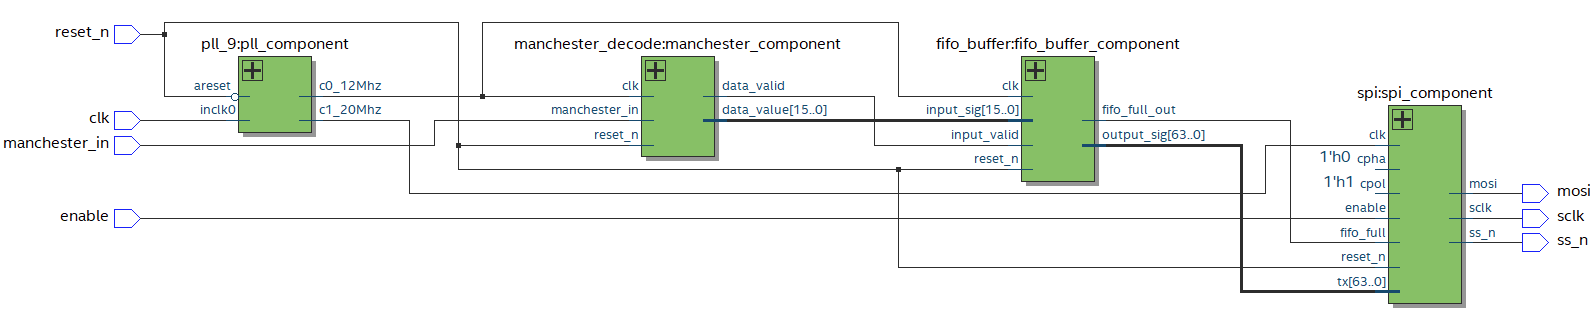
\includegraphics[width=1\linewidth]{Figures/Chap3/FPGA/FPGA_Darstellung_Projekt.png}
    \caption{Aufbau des VHDL-Codes in Blockschaltbildern}
    \label{fig:AufbauFPGA}
\end{figure}

In den folgenden Unterkapiteln werden die einzelnen wichtigsten Prozesse genauer erklärt.\\
\\
Dabei ist wichtig zu erwähnen, dass durch die Decodierung des Manchestersignal, aus einem Bit
(Manchester-Codiert) zwei Bit (Bitstream) werden. Das heisst im 16 Bit grossen 
\textit{data\_value\_reg} ist jeweils ein Byte des MVB abgebildet.\\
\newline
In dieser Arbeit gelten folgende Einheitsnamen und Datengrössen:\\
\textbf{Nutzdatenbyte}\hspace{0.1cm}= \textbf{8 Bit} (Manchester) =\hspace{0.1cm}\textbf{16 Bit} (decodiertes Signal) in \textit{data\_value\_reg}\\
\textbf{Nutzdatenbit}\hspace{0.37cm}= \textbf{1 Bit} (Manchester) =\hspace{0.3cm}\textbf{2  Bit} (decodiertes Signal)
\newpage
\subsection{Manchester Decodierung}
\label{Manchester Decodierung}

Um das Manchestersignal decodieren zu können, muss dieses abgetastet werden. Um möglichst synchron zum
Signal vom MVB zu sein muss die Abtastfrequenz ein Mehrfaches der MVB Bitrate sein. Um die Abtastung möglichst
robust zu machen und Fehler zu vermeiden wurde festgelegt minimal vier mal pro Flanke abzutasten. Somit
wird verhindert dass durch ungewolltes shiften und bei einer Abtastung genau auf dem Flankenwechsel, falsche Werte
decodiert werden.
Bei einer Abtastung von vier mal pro Flanke und somit acht mal pro BT (666 ns = 1.5 MHz) ergibt sich eine Abtastfrequenz von 12 MHz.
Um diese Abtastrate zu realisieren, wurde mit der Designsoftware Quartus eine Taktfrequenz von 12 MHz generiert.
Die abgetasteten Werte werden fortlaufend in ein acht Bit grosses Register \textit{reg\_sample} geschrieben.
In Abbildung \ref{fig:MasterframeAbtastung} ist das Master Start-Delimiter mit den
jeweiligen Abtastpunkten in blau, den Abtastwerten im Register \textit{reg\_sample} von Bit 0 - 7 und den darauffolgenden decodierten 
Werte, welche ins 16 Bit grosse Register \textit{data\_value\_reg} geschrieben werden, zu sehen.
%Immer nach acht Zyklen werden die Daten in diesem Register ausgewertet.

\begin{figure}[H]
    \centering
    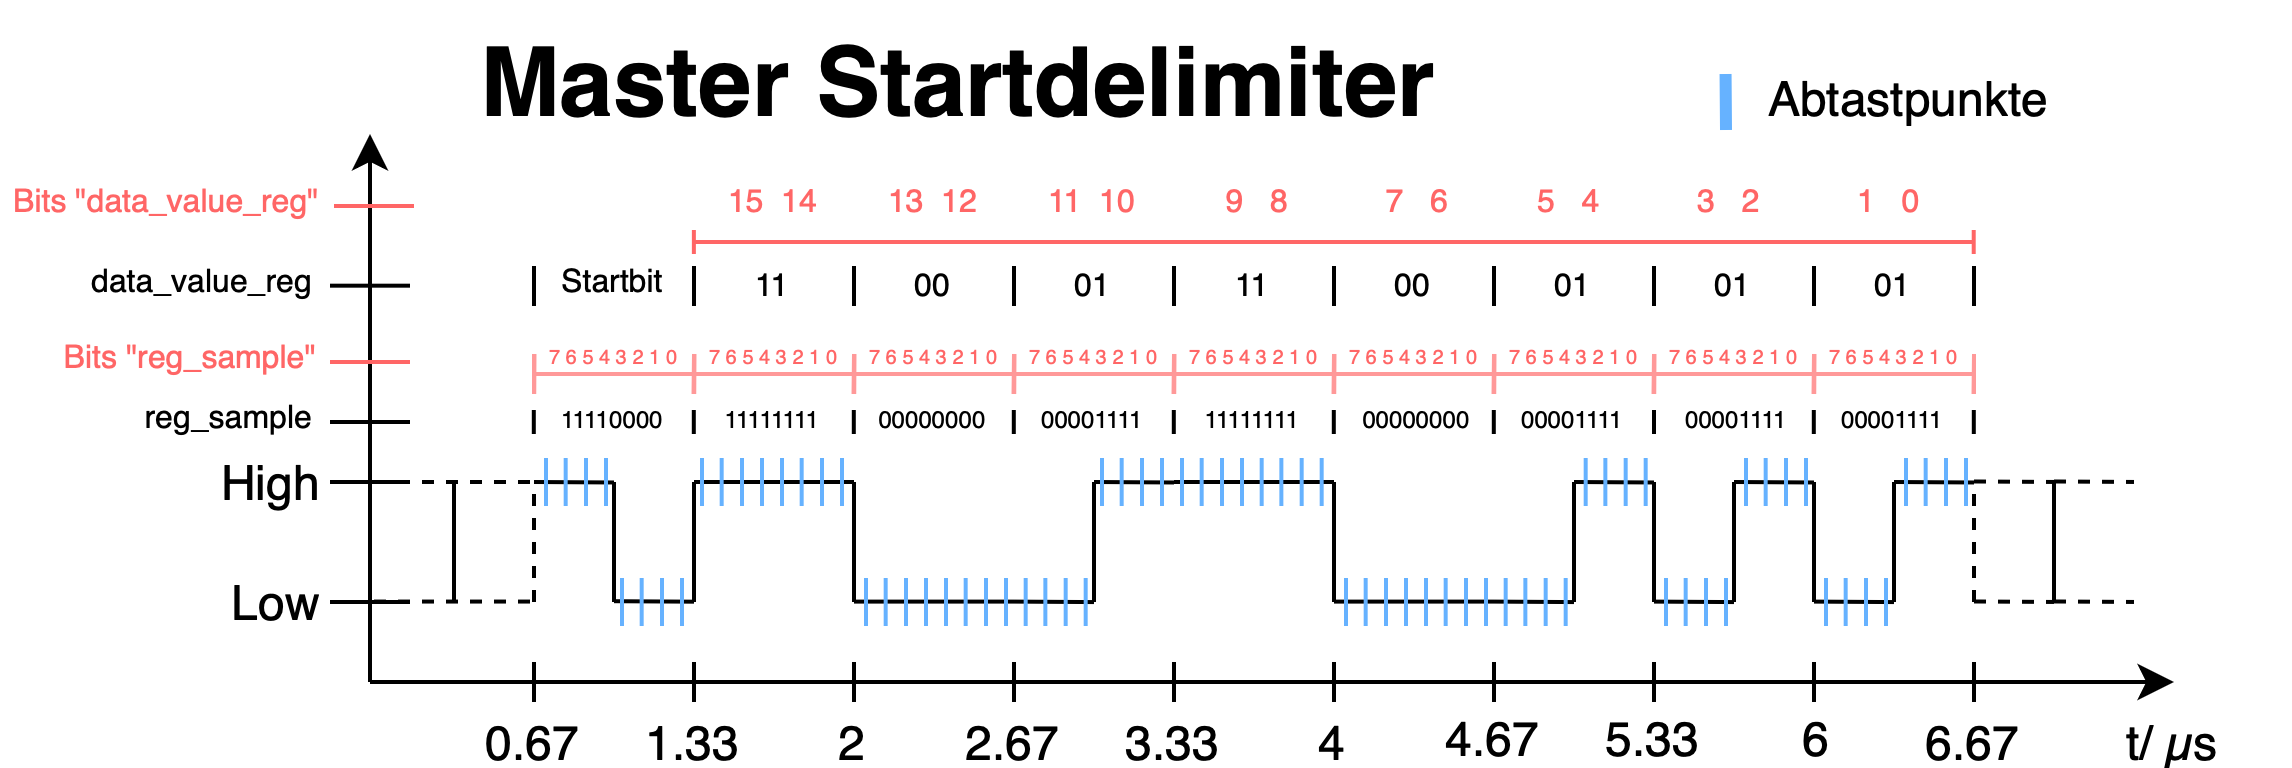
\includegraphics[width=1\linewidth]{Figures/Chap3/FPGA/Abtastpunkte_Master.png}
    \caption{Master-Frame Start-Delimiter mit Abtastpunkten}
    \label{fig:MasterframeAbtastung}
\end{figure}

\subsubsection{Auswertung Manchestersignal}
\label{Auswertung Manchestersignal}
Immer zu Beginn eines Frame (Master wie auch Slave) wird der Start mit einem Startbit signalisiert, wie dies bereits in Kapitel \ref{sub:StartDelimiter} beschrieben ist.
Sobald das \textit{Start bit} im Auswerteprozess erkannt wird, heisst sobald Bit 5 - 2 im Register \textit{reg\_sample} den Wert \textit{"'1100"'} haben, wechselt das FPGA vom Zustand \textit{IDLE} in den Zustand \textit{RECEIVING}. Dieser Zustandswechsel ist in Abbildung \ref{fig:FPGAIdleRec} dargestellt.

\begin{figure}[H]
    \centering
    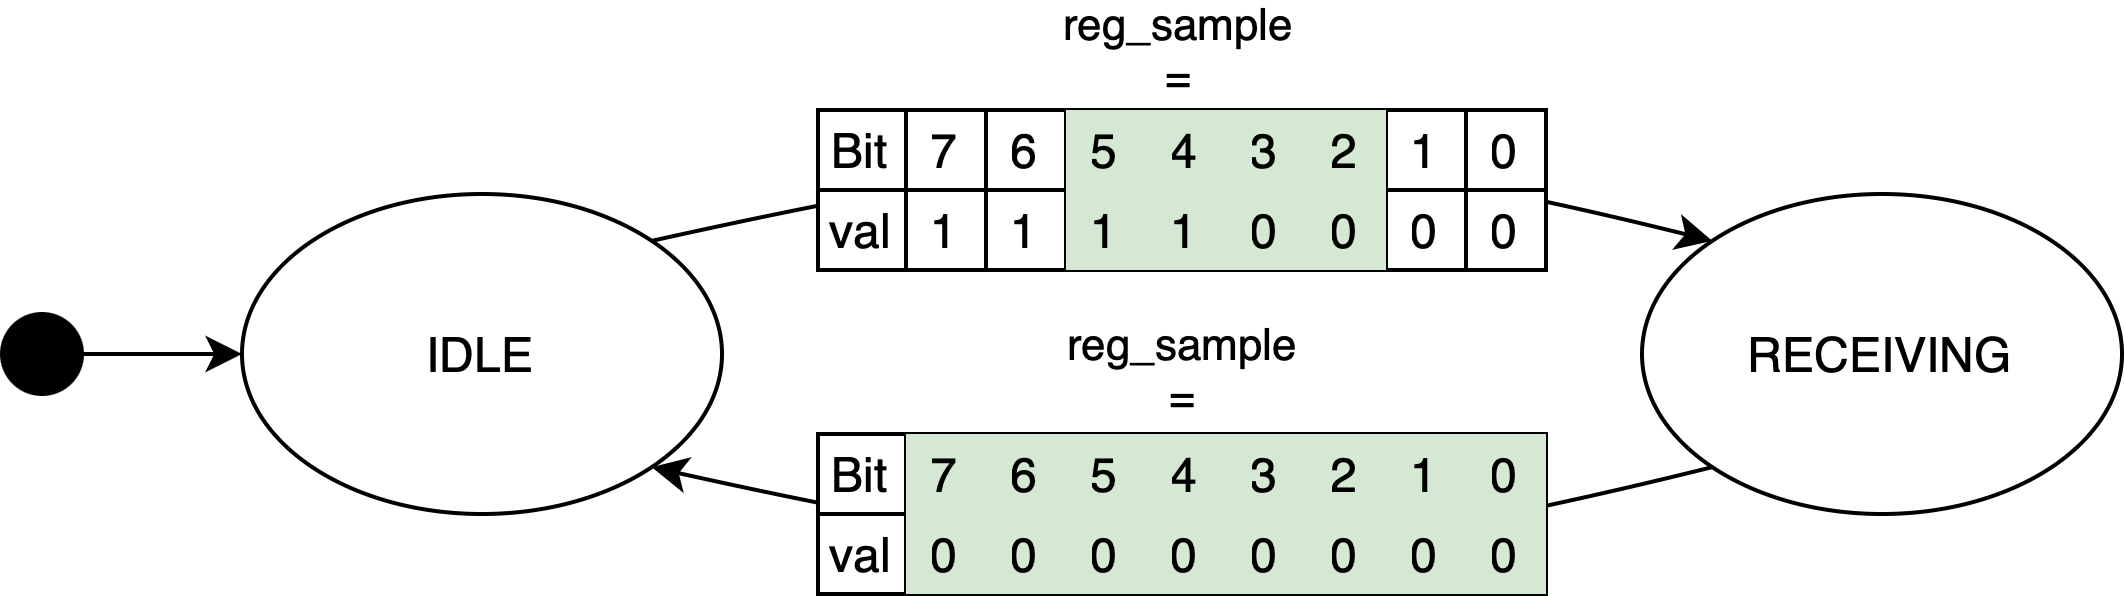
\includegraphics[width=0.7\linewidth]{Figures//Chap3//FPGA/FPGA_idle_rec.png}
    \caption{Zustandsdiagramm FPGA Manchester-Decodierung}
    \label{fig:FPGAIdleRec}
\end{figure}

Im Zustand \textit{RECEIVING} werden Fortlaufend die abgetasteten Werte ins Register 
\textit{reg\_sample} geschrieben und immer nachdem acht mal abgetastet wurde, werden die Daten in diesem Register ausgewertet. Dabei ist im Idealfall immer ein ganzes BT des MVB-Signal im Register abgebildet, was einem Nutzdatenbit entspricht. Idealerweise ist dann auch der Übergang der Flanke von "'0"' auf "'1"' oder von "'1"' auf "'0"' genau bei Bit 4 auf 3 zu sehen. Die Auswertelogik überprüft dann jeweils was an den Stellen 5 - 2 des Registers steht und schreibt dementsprechend die Werte weiter ins Register \textit{data\_value\_reg}. Im Idealfall gibt es dann genau vier Fälle die entstehen können.


% Das sind die folgenden vier:

% \textbf{Fall 1}\\
% Bei einem Übergang von '0' auf '1' beinhaltet \textit{reg\_sample} die Werte \textit{"'00001111"'}. Somit ist bei bit 4 auf 3 der Übergang "'01"' zu sehen. Das ist gleichzeitig der Wert welcher ins \textit{data\_value\_reg} geschrieben wird.

% \textbf{Fall 2}\\
% Bei einem Übergang von '1' auf '0' beinhaltet \textit{reg\_sample} die Werte \textit{"'11110000"'}. Hier ist bei bit 4 auf 3 eine "'10"' zusehen.

% \textbf{Fall 3}\\
% Fall drei deckt die erste violation ab. Heisst wenn das Register nur mit Nullen gefüllt ist \textit{"'00000000"'}. In diesem Fall wird ins \textit{data\_value\_reg} der Wert "'00"' geschrieben.

% \textbf{Fall 4}\\
% Im vierten Fall wird die zweite violation erkannt. Wenn das Register die Werte \textit{"'11111111"'} beinhaltet wird ins \textit{data\_value\_reg} der Wert "'11"' geschrieben.

Da der Abtasttakt nicht synchron mit dem MVB-Takt läuft kann es zu leichten Abweichungen kommen, was dazu führt dass der Flankenwechsel nicht bei Bit 4 auf
3 sondern bei Bit 3 auf 2 oder bei Bit 5 auf 4 zu sehen ist. Um diese weiteren Fälle abzufangen, werden jeweils nicht nur die 
mittleren zwei Bit auf ihre Werte überprüft, sondern gleich die mittleren vier Bit. Somit überprüft der Auswerteprozess das Register nicht nur auf vier, sondern auf acht Fälle.

Da das Register \textit{data\_value\_reg} 16 Werte beinhaltet würde es noch weitere acht Fälle
geben. Das Eintreffen der weiteren Acht Fälle wird durch ein shiften der Bit, wenn das Signal über
drei Auswertezyklen hinweg nicht synchron läuft, verhindert. Somit muss die Auswertelogik Acht
Fälle implementiert haben und diese korrekt abarbeiten.

In Abbildung \ref{fig:FPGAreg_sampleCases} sind alle 16 möglichen Fälle zu 
sehen, welche das Register \textit{data\_value\_reg} annehmen könnte, wenn davon 
ausgegangen wird, dass keine Korrektur durch Shifting implementiert ist und wenn
alle 16 Bit zur Auswertung betrachtet würden.

\begin{figure}[H]
    \centering
    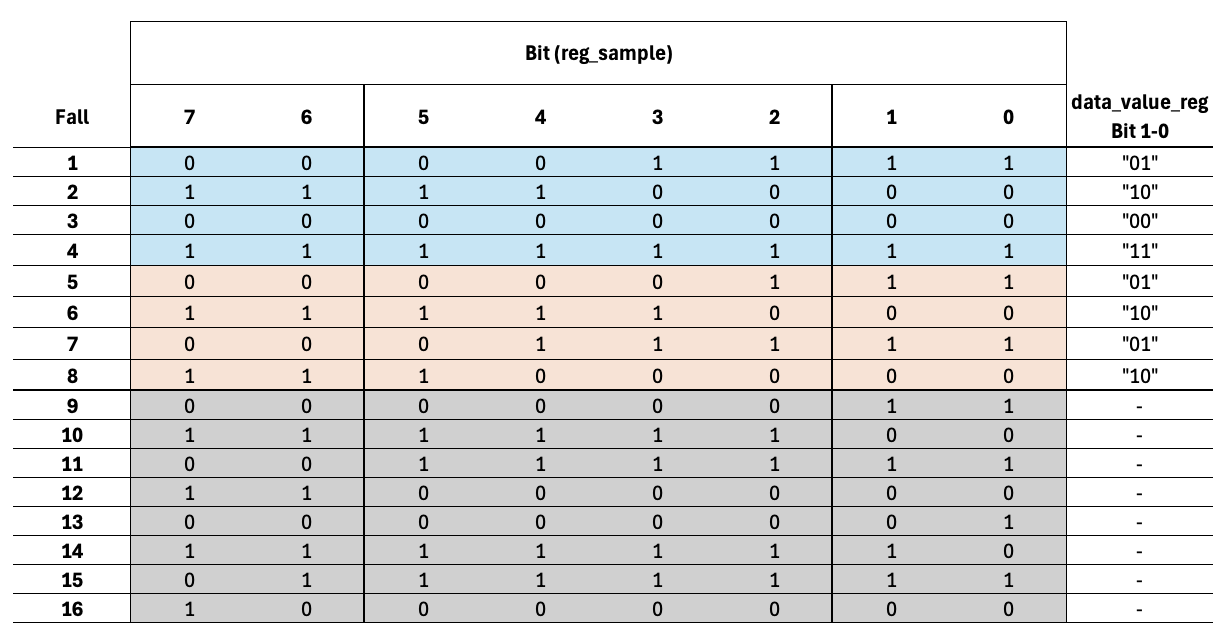
\includegraphics[width=1\linewidth]{Figures//Chap3//FPGA/FPGA_decoding_case.png}
    \caption{Darstellung der Fälle welche das Register \textit{reg\_sample} annehmen kann}
    \label{fig:FPGAreg_sampleCases}
\end{figure}

In Abbildung \ref{fig:FPGAreg_sampleCases} ist zu sehen, dass bei den ersten vier
Fällen genau ein ganzes Nutzdatenbyte im Register abgebildet ist und somit der 
Flankenwechsel bei Bit 4 auf Bit 3 zu sehen ist. In diesen Fällen ist kein 
nachträgliches Shifting nötig und der Wert, welcher in der letzten Spalte zu
sehen ist wird ins \textit{data\_value\_reg} Register geschrieben.

In den Fällen fünf bis acht sind die Werte jeweils um ein Bit verschoben, wodurch
der Flankenwechsel bei Bit 3 auf 2 (Fall 5 \& 6) oder bei Bit 5 auf 4
(Fall 7 \& 8) statt findet. Diese Fälle werden erkannt und die jeweiligen Werte, wie
sie in der letzten Spalte zu sehen sind, ins Register \textit{data\_value\_reg} 
geschrieben.\\
In diesen Fällen notwendig. Dieser Prozess wird in Kapitel \ref{Shifting-Prozess}
erläutert.

In den Fällen neun bis 16 sind die Werte um zwei oder um drei Bit verschoben. Diese Fälle würden dann auftreten, wenn sich das MVB-Signal innerhalb von acht
Abtastungen um zwei ganze Abtastwerte verschiebt. Dies entspricht einer
Verschiebung um 25 \%. In der Norm IEC 61375-3-1 ist festgehalten dass eine maximale Abweichung zur Taktfrequenz 1.5 MHz um 0.01 \% vorkommen kann. \cite{MVB_Norm}\\
Daher werden die Fälle 9 bis 16 nie erreicht und müssen nicht in der Auswertelogik
implementiert sein.
 
%  Folgend die Fälle fünf bis acht:

% \textbf{Fall 5}\\
% Ist durch eine Verschiebung nun der Übergang von Bit 5 auf 4 zu sehen, heisst beinhaltet das Register \textit{reg\_sample} die Werte \textit{"'00011110"'}, wird das erkannt und es wird gleichermasen ein "'01"' ins \textit{data\_value\_reg} geschrieben.

% \textbf{Fall 6}\\
% Bei Fall sechs ist der übergang wieder am gleichen Ort wie bei Fall fünf. Nun aber wird eine "'10"' erkannt und ins \textit{data\_value\_reg} geschrieben.

% \textbf{Fall 7}\\
% Im siebten Fall ist der Übergang nun bei Bit 3 auf 2. Es ergibt sich das Register \textit{reg\_sample} welches die Werte \textit{"'01111000"'} beinhaltet und somit den Wert "'01"' schreibt.

% \textbf{Fall 8}\\
% Im letzten Fall ist der Übergang wieder am gleichen Ort wie in Fall sieben, aber nun wird ein "'10"' erkannt und dann auch ins Register \textit{data\_value\_reg} geschrieben.

% Trifft bei der Auswertung einer der Fälle 5 - 8 zu, so wird entweder die Variable \textit{shift\_up} oder \textit{shift\_down} auf '1' gesetzt und weiter an den Prozess \textit{shifting} übergeben, welcher die Abweichung aktiv korrigiert.

Die erläuterte Auswertelogik ist unten, in VHDL implementiert, zu sehen:

\begin{lstlisting}[language=vhdl]
decode_proc: PROCESS (clk, reset_n)
BEGIN		
    IF(reset_n = '0') THEN
       data_value_reg <= (others => '0');
       shift_up <= '0';
       shift_down <= '0';	
    ELSIF(rising_edge(clk)) THEN
       shift_up <= '0';
       shift_down <= '0';
       IF state = RECEIVING THEN
    	   IF count_sample = 0 THEN
    	      data_value_reg(15 DOWNTO 2) <= data_value_reg(13 DOWNTO 0);
    	      IF reg_sample(5 DOWNTO 2) = "0011" THEN
    	         data_value_reg(1 DOWNTO 0) <= "01";
    	      ELSIF reg_sample(5 DOWNTO 2) = "1100" THEN
    	         data_value_reg(1 DOWNTO 0) <= "10";
    	      ELSIF reg_sample(5 DOWNTO 2) = "0001" THEN
    	         data_value_reg(1 DOWNTO 0) <= "01";
    	         shift_up <= '1';
    	      ELSIF reg_sample(5 DOWNTO 2) = "1110" THEN
    	         data_value_reg(1 DOWNTO 0) <= "10";
    	         shift_up <= '1';
    	      ELSIF reg_sample(5 DOWNTO 2) = "0111" THEN
    	         data_value_reg(1 DOWNTO 0) <= "01";
    	         shift_down <= '1';
    	      ELSIF reg_sample(5 DOWNTO 2) = "1000" THEN
    	         data_value_reg(1 DOWNTO 0) <= "10";
    	         shift_down <= '1';
    	      ELSIF reg_sample(5 DOWNTO 2) = "0000" THEN
    	         data_value_reg(1 DOWNTO 0) <= "00";
    	      ELSIF reg_sample(5 DOWNTO 2) = "1111" THEN
    	         data_value_reg(1 DOWNTO 0) <= "11";
              END IF;
    	   END IF;
       END IF;		
    END IF;
END PROCESS;
\end{lstlisting}

\newpage

\subsubsection{Shifting-Prozess}
\label{Shifting-Prozess}
Wie in Kapitel \ref{Manchester Decodierung} erwähnt, müssen in einigen Fälle mehr oder weniger
Werte ins Register \textit{reg\_sample} geschrieben werden. Diese Aufgabe wird in einem
separaten Prozess abgearbeitet. Es wird geprüft wie oft \textit{shift\_up} in Fall 5 \& 6 bzw. \textit{shift\_down} in Fall 7 \& 8 auf '1' gesetzt wurde.
In Abbildung \ref{fig:FPGAShiftingCases} sind die Fälle bei denen ein Shifting notwendig ist
zu sehen. In grün eingefärbt ist zu sehen wann \textit{shift\_up} und \textit{shift\_down}
gesetzt werden und in welche Richtung \textit{count\_shift} zählt.

\begin{figure}[H]
    \centering
    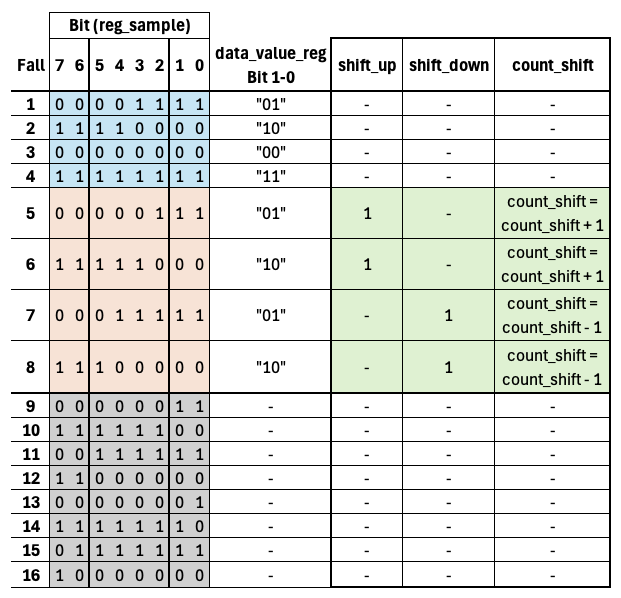
\includegraphics[width=0.9\linewidth]{Figures//Chap3//FPGA/FPGA_Shifting.png}
    \caption{Fälle in denen ein Shifting der Bit notwendig ist}
    \label{fig:FPGAShiftingCases}
\end{figure}

% Dies geschieht mit einem counter \textit{count\_shift}, welcher im Falle \textit{shift\_up} den Zählerwert um eins erhöht und im Falle \textit{shift\_down} um eins reduziert.
Sobald \textit{count\_shift} den Wert "'2"' drei mal übersteigt so wird das Register \textit{reg\_sample} das nächste mal nicht nach acht, sondern nach sieben mal ausgewertet. Falls der Zählerwert, ebenfalls drei mal, den Wert "'-2"' unterbietet so wird die nächste Auswertung der Werte nach neun Abtastwerten statt finden. Mit dieser Logik wird aktiv überprüft ob der Flankenwechsel immer in der Mitte des \textit{reg\_sample} Registers zu erkennen ist und falls dies drei mal hintereinander nicht der Fall ist, so wird reagiert und ein Bit mehr oder weniger ins Register geschrieben.
Nach der Korrektur wird der Counter \textit{count\_shift} wieder auf '0' gesetzt. Es wird
erst nach drei mal reagiert, um somit zu verhindern dass die Logik bei einer einmaligen 
Abweichung durch falsches shiften die Abweichung noch grösser macht und sich somit sehr oft
selbst korrigieren muss.

\newpage
Die Implementierung des Shifting-Prozess in VHDL ist folglich zu sehen:

\begin{lstlisting}[language=vhdl]
shift_proc: PROCESS (clk, reset_n)
BEGIN		
	IF(reset_n = '0') THEN
		samples_per_bit <= to_unsigned(7, 4);
		count_shift <= (others => '0');
	ELSIF(rising_edge(clk)) THEN
		IF state = IDLE THEN
			samples_per_bit <= to_unsigned(7, 4);
			count_shift <= (others => '0');
		ELSE	
			IF shift_up = '1' THEN
				count_shift <= count_shift + 1;
			ELSIF shift_down = '1' THEN
				count_shift <= count_shift - 1;
			END IF;
			IF count_shift > 2 THEN
				samples_per_bit <= to_unsigned(8, 4);
				count_shift <= (others => '0');
			ELSIF count_shift < -2 THEN
				samples_per_bit <= to_unsigned(6, 4);
				count_shift <= (others => '0');
			END IF;
			IF count_sample = 0 THEN
				samples_per_bit <= to_unsigned(7, 4);
			END IF;	
		END IF;
	END IF;
END PROCESS;
\end{lstlisting}

\subsection{SPI}
\label{fpga:spi}
Damit die Daten aus dem Register \textit{data\_value\_reg} für die weitere Auswertung und Verarbeitung an den Mikrocontroller ESP32-S3 übertragen werden können, wurde das Übertragungsprotokoll SPI implementiert.\\
\\
Als Basis zum VHDL-Code wurde die bereits geschriebene SPI-Master Implementierung von Github genommen und angepasst. \cite{SPI_git}


Es wurde festgelegt, dass das FPGA als Master und der ESP32-S3 als Slave agiert. Als Modi wurden \textit{CPOL=0} und \textit{CPHA=0} bestimmt. Die Übertragungsfrequenz wurde möglichst hoch gewählt, damit die Daten sicherlich schneller übertragen, als die neu abgetasteten Werte wieder ins Register geschrieben, werden.
Das FPGA sowohl als auch der ESP32-S3 mussten die Frequenz erreichen können. Schlussendlich wurde 20 MHz als Übertragungsrate festgelegt.

Werden immer, sobald das Register \textit{data\_value\_reg} voll ist, die Daten auf das SPI übertragen, so würden alle \textit{5.33 µs} neue Daten übertragen werden. Die Zahl berechnet sich folgendermassen:
% Requires: \usepackage{siunitx}

\begin{equation}
    8 \, \text{ Nutzdatenbit} \times 666 \, \text{ ns} = 5328 \, \text{ ns} = 5.33 \text{ }  \mu\text  s \label{eq:calc_Nutzdatenbit1}
\end{equation}

Da der ESP32-S3 nur alle \textit{16 µs} neue Daten empfangen kann (siehe Kapitel \ref{sec:ResultatESP32}) wurde entschieden, dass das FPGA die Daten jeweils puffert und sobald der Puffer von 32 Nutzdatenbits voll ist, diesen auf das SPI überträgt. Damit ergibt sich folgende Zeit zwischen den Übertragungen:

\begin{equation}
    32 \, \text{ Nutzdatenbit} \times 666 \, \text{ ns} = 21312 \, \text{ ns} = 21.3 \text{ }  \mu\text s \label{eq:calc_Nutzdatenbit2}
\end{equation}

Unterhalb ist die Logik für das Schreiben des Puffers in VHDL zu sehen:
\begin{lstlisting}[language=vhdl]
PROCESS(clk, reset_n)
BEGIN
    IF reset_n = '0' THEN
        fifo <= (others => (others => '0'));
        write_ptr <= 0;
        fifo_full <= '0';
        buffer_ready <= '0';
        output_sig <= (others => '0');
    ELSIF rising_edge(clk) THEN
        IF input_valid = '1' and fifo_full = '0' THEN
            fifo(write_ptr) <= input_sig;
            write_ptr <= write_ptr + 1
            IF write_ptr = 3 THEN
                fifo_full <= '1';
                buffer_ready <= '1';
            ELSE
                buffer_ready <= '0';
            END IF;
        END IF;
        IF fifo_full = '1' THEN
            output_sig <= fifo(0) & fifo(1) & fifo(2) & fifo(3);
            fifo_full <= '0';
            write_ptr <= 0;
        END IF;
    END IF;
END PROCESS;
\end{lstlisting}

Wodurch der ESP32-S3 genug Zeit für die Verarbeitung hat und somit alle Daten korrekt und ohne Verlust übertragen werden können.

%----------------------------------------------------------------------
% SECTION Firmware ESP32
%----------------------------------------------------------------------

\section{Firmware ESP32}
%\textcolor{red}{Wie wurde die Firmware auf dem ESP32 umgesetzt? Kurze Einleitung noch schreiben}

Die Firmware für den ESP32-S3 wurde mithilfe der ESP-IDF, dem IoT Development Framework, geschrieben. Dabei wurde die Integration von FreeRTOS sowie das Aufsetzen eines Bluetooth GATT-Servers programmiert. 

In Abbildung \ref{fig:FSMEinleitung} ist der Aufbau der Firmware grob schematisch zu sehen. Der Einstiegspunkt bietet dabei die \textit{app\_main()} Funktion, welche die Peripherien initialisiert und drei Tasks erstellt. Die main()-Funktion ist damit abgeschlossen und der Scheduler übernimmt die restliche Ausführung des Programms. Das Symbol in der rechten unteren Ecke in T2 zeigt an, dass dieser Task eine Statemachine umfasst. Auf die verschiedenen Tasks wird in diesem Abschnitt eingegangen.

\begin{figure}[H]
    \centering
    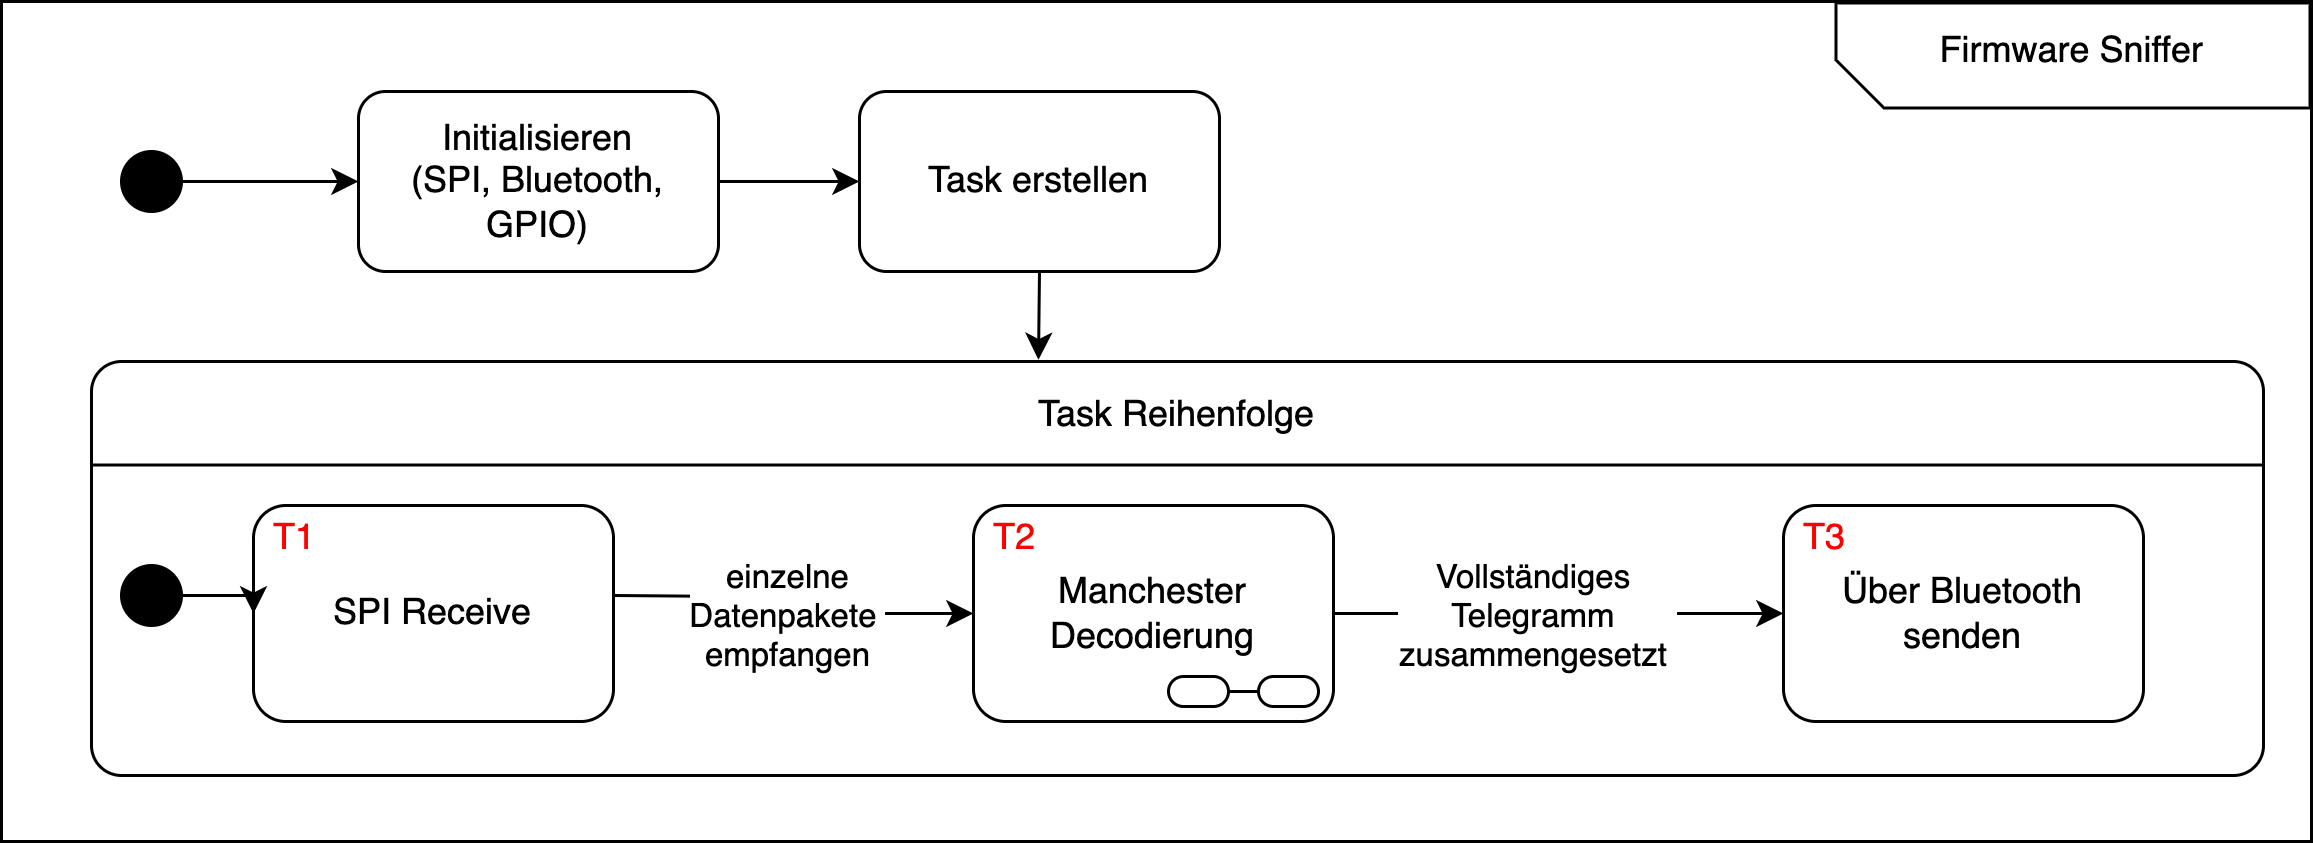
\includegraphics[width=0.9\linewidth]{Figures/Chap3/ESP/Einleitung/FSM_Einleitung.png}
    \caption{Ablaufdiagramm Firmware Sniffer von Programmeinstieg bis Task}
    \label{fig:FSMEinleitung}
\end{figure}

\subsection{Real Time Operating System (FreeRTOS) auf ESP32}
%\textcolor{red}{Wie wurde das FreeRTOS benutzt, um die Zeitkritische Aufgaben zu lösen? Welche Tasks und welche FSM arbeiten in den jeweiligen Cores?}


Für dieses Projekt kam FreeRTOS zum Einsatz, das bereits in der ESP-IDF, der Entwicklungsumgebung für den ESP32-S3, integriert ist. \cite{FREERTOS_IDF_API} In diesem Abschnitt werden die Umsetzung des Betriebssystems und die genutzten FreeRTOS-Elemente beschrieben, um den Betrieb zu ermöglichen.

\subsubsection{Task}
Es werden Tasks definiert, welche von einem Scheduler anschliessend gemanagt und aufgerufen werden. Für die Ausführung der Hauptaufgaben auf dem Sniffer wurden 3 Tasks gemäss Tabelle \ref{tab:TaskDefinitonen} definiert.

\begin{table}[H]
    \centering
    \begin{tabular}{|c||c|c|c|}
        \hline
        Funktionspointer & spi\_receive  & mvb\_manch\_decode & bt\_send\\ 
        \hline
        Name Task  & "'spi\_receive"' & "'mvb\_manch\_decode"' & "'bt\_send"'\\ 
        \hline
        Stackgrösse & 10000 & 10000 & 10000\\ 
        \hline
        Parameter & NULL & NULL & NULL\\ 
        \hline
        Priorität & 3 & 2 & 1\\ 
        \hline
        Handle & NULL & NULL & NULL\\ 
        \hline
    \end{tabular}
    \caption{Task Definitionen FreeRTOS}
    \label{tab:TaskDefinitonen}
\end{table}

Der Task \textit{spi\_receive} und \textit{mvb\_manch\_decode} erhalten beide eine grössere Priorität als der Task \textit{bt\_send}. Wie in Abbildung \ref{fig:ReineDaten} zu sehen ist, gibt es Zeitabschnitte, in denen viele Daten verarbeitet werden müssen, gefolgt von einer Idle-Periode. In der Idle-Zeit hat der Task \textit{bt\_send} die Möglichkeit, Telegramme über Bluetooth herauszuschicken und soll nicht in einer Periode, wo viele Daten kommen, die CPU beanspruchen.


\subsubsection{Queue}
\label{subsub:Queue}
Für den primären Datenaustausch zwischen den Tasks werden Queues verwendet. Wenn ein Task von einer leeren Queue lesen will, wird dieser in den \textit{blocking-state} versetzt. Dadurch gibt dieser Task die CPU frei und wird erst wieder aufgerufen, wenn sich ein Element in der Queue befindet.\cite{FREERTOS_QUEUE}

Für die Intertask-Kommunikation wurden zwei Queue definiert. In Abbildung \ref{fig:QueueSchema} ist eine schematische Darstellung des Datenflusses gezeigt.


\begin{figure}[H]
    \centering
    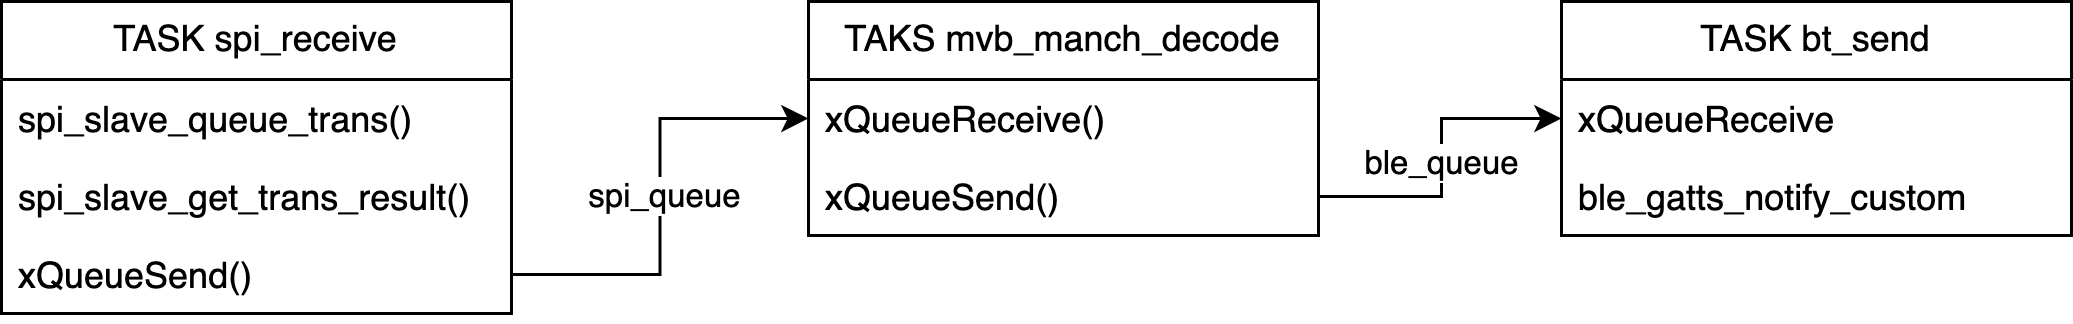
\includegraphics[width=0.9\linewidth]{Figures/Chap3/ESP/FreeRTOS/Queue.png}
    \caption{Schematische Darstellung der verwendeten Queues}
    \label{fig:QueueSchema}
\end{figure}

Die \textit{spi\_queue} fasst 64 Werte à 16 Bit. Die Wahl von 16 Bit basiert auf der Verarbeitung durch den Task \textit{mvb\_manch\_decode}. Die Grösse von 64 wurde gewählt, damit ein möglichst grosser Buffer ansteht und keine Daten verloren gehen können.

Die \textit{ble\_queue} fasst acht Pointer auf \textit{struct telegramm}. Pointer werden verwendet, da sie mit 4 Bytes deutlich speicherplatzeffizienter sind als das 40 Byte grosse \textit{struct}. Die Grösse acht entspricht dem in Kapitel \ref{subsub:DataTelegramm} erstellten Arrays. So wird sichergestellt, dass Werte in der Queue nicht überschrieben werden, bevor sie über Bluetooth übertragen werden.

\subsection{Global verwendete Datenstrukturen}
\label{sub:GlobalDtatStruct}
Für die Zwischenspeicherung der Telegrammdaten und das Empfangen von SPI-Daten werden zwei globale Datenstrukturen erstellt, welche die Speicherung und die Lesbarkeit verbessern. 

\subsubsection{Datentyp Telegramm}
\label{subsub:DataTelegramm}
Für das Zusammensetzen der Telegramme wurde nachfolgendes \textit{struct} in C definiert.

\begin{lstlisting}[language=C]
typedef struct telegramm
{
    uint8_t metadata;       // Fehler im Telegramm (Bsp 0x01: Nur Master-Frame)
    uint8_t data_m[2];      // Master-Frame Daten
    uint8_t check_m;        // Master Check Sequenz
    uint8_t data_s[32];     // Slave-Frame Daten eines 256 Bit
    uint8_t check_s[4];     // Slave Check Squenzen
} telegramm;
\end{lstlisting}

Die Metadaten sind ein Bereich, indem ungültige Telegramme oder Fehler übermittelt werden können. Die restlichen Daten entsprechen dem grössten Telegramm mit einem Slave-Frame von 256 bit gemäss Kapitel \ref{fig:SlaveFrameFormat}. Somit ist es möglich, alle Arten von Telegrammen zu speichern. Dies kann zukünftig verbessert werden, indem nur der für das Telegramm benötigte Speicherplatz verwendet wird. 

Ein Array mit dem Makro \textit{MAX\_MESSAGES} wurde erstellt und ist global für das ganze Programm zugreifbar. 

\begin{lstlisting}[language=C]
#define MAX_MESSAGES 8

telegramm messages_tel[MAX_MESSAGES] = {0};
\end{lstlisting}

Damit wurde ein Speicherbereich für 8 Telegramme initialisiert. Das Array-Element wird im Task \textit{mvb\_manch\_decode} beschrieben und der Pointer auf das neu beschriebene Element aus dem Array über die ble\_queue dem Task \textit{bt\_send} weitergegeben. 


\subsubsection{Union SPI-Receive}
\label{subsub:UnionSPI}

Der Buffer mit den empfangenen Daten von der SPI-Transaktion ist Little Endian. Für die Verarbeitung von jeweils 16 Bit müssen die Bytes jedoch noch vertauscht werden. Zu diesem Zweck wurde folgende Union in C gebildet.

\begin{lstlisting}[language=C]
union u_tel_message
{
    // Emfangen von SPI Daten
    uint32_t spi_rec[2];

    // Zugriff auf Bytes
    struct 
    {
        uint8_t byte0;
        uint8_t byte1;
        uint8_t byte2;
        uint8_t byte3;
        uint8_t byte4;
        uint8_t byte5;
        uint8_t byte6;
        uint8_t byte7;
    } bytes;
};
\end{lstlisting}

Die Union wird nur vom Task \textit{spi\_receive} verwendet. Die Verwendung wird in Kapitel \ref{sub:TaskSPIReceive} gezeigt. 


\subsection{Task - SPI Receive}
\label{sub:TaskSPIReceive}
Der ESP32-S3 verfügt über eine SPI-Schnittstelle, die für den Empfang von Daten verwendet wird. Im Rahmen dieses Projekts wurde ein 4-Buffer-System implementiert, basierend auf einem Beitrag\cite{ESP_FORUM_SPI_BUFFER}, um die Datenverwaltung effizient zu gestalten. 4 wurden gewählt, weil dies in Tests die geringste Anzahl an Fehltransaktionen zeigte.

Zusätzlich wurde ein Handshake-Pin integriert, der in einem Callback sowohl während der Initialisierung (\textit{setup}) als auch nach der Transaktion verwendet wird. Ein High-Signal (1) signalisiert, dass der SPI-Empfänger aufnahmebereit ist, während ein Low-Signal (0) anzeigt, dass sich der Empfänger in der Verarbeitung befindet.

In Abbildung \ref{fig:3BuffKonz} ist eine schematische Illustration davon dargestellt. 

\begin{figure}[H]
    \centering
    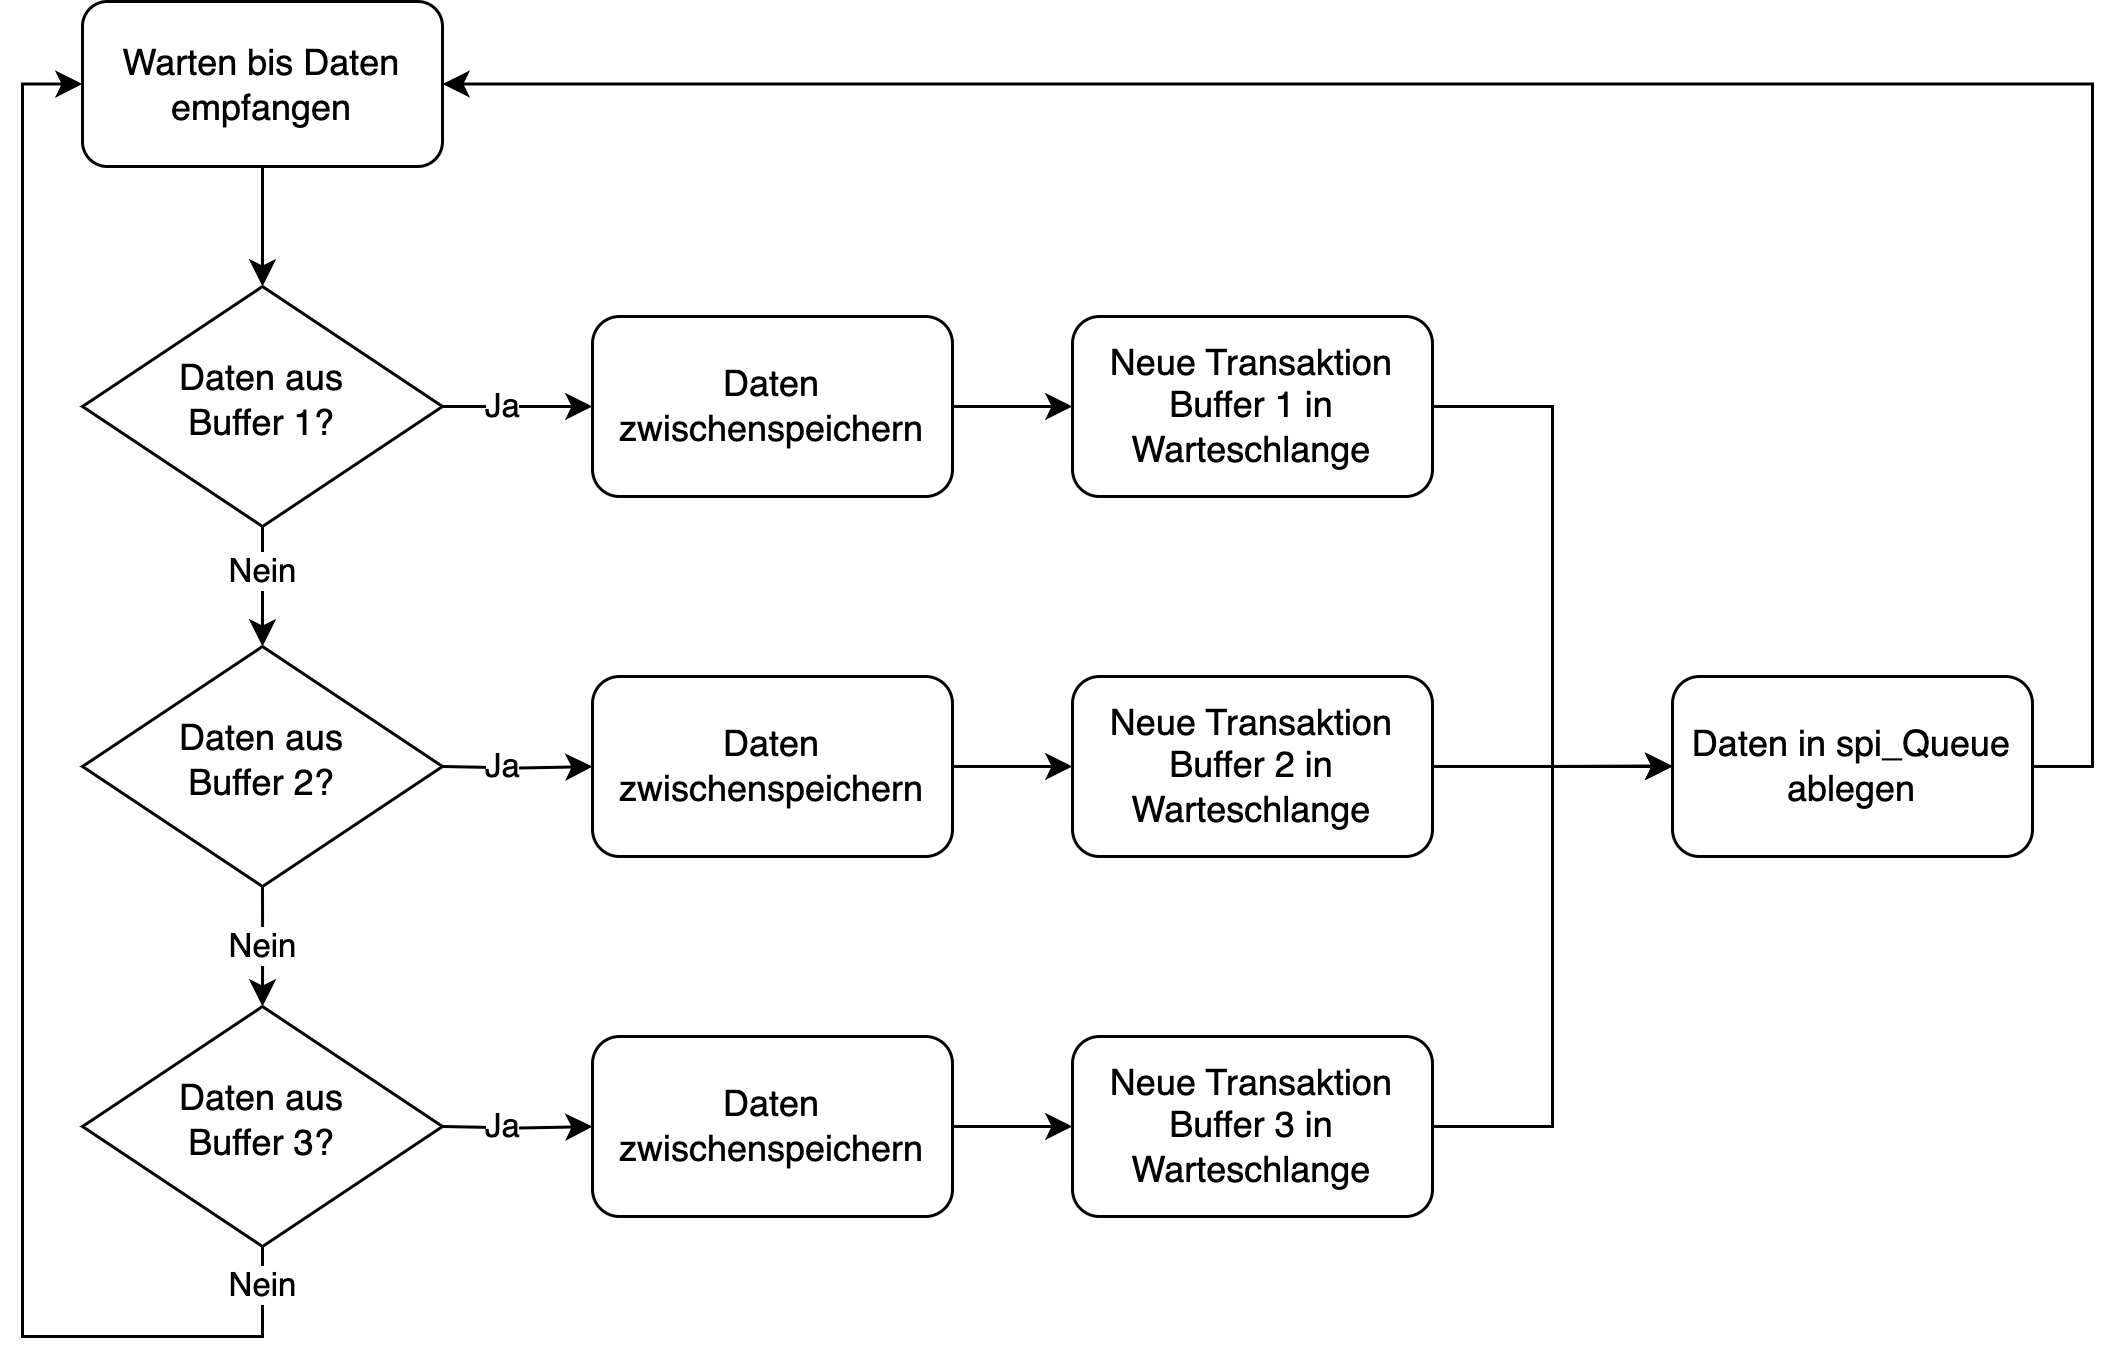
\includegraphics[width=0.75\linewidth]{Figures/Chap3/ESP/SPI_RECEIVE/Bufferkonzept_BLE.png}
    \caption{3-Buffer-Konzept SPI empfangen}
    \label{fig:3BuffKonz}
\end{figure}

Zur Weitergabe der empfangenen Daten in die \textit{spi\_queue} wird die in Kapitel \ref{subsub:UnionSPI} beschriebene Union verwendet.

Der folgende Codeausschnitt zeigt exemplarisch die Verarbeitung eines Buffers, einschliesslich der Nutzung der Union und des Empfangs von Daten:

\begin{lstlisting}[language=C]
/* FreeRTOS TASK */
void spi_receive(void *pvParameters)
{
    //...
    
    while (true)
    {
        // Programm geht nicht weiter, wenn keine Daten Empfangen werden.
        spi_slave_get_trans_result(RCV_HOST, &trx_ptr, portMAX_DELAY);

        // Abgleich Buffer
        if (trx_ptr->user == t1_ptr->user)
        {
            u_message.spi_rec[0] = receive_data1[0];
            u_message.spi_rec[1] = receive_data1[1];
            spi_slave_queue_trans(RCV_HOST, &t1, 0);
        } 
        else if
        {
        // ... Weitere Receive Buffer
        }
        else
        {
            // Daten liegen in keinem Gueltigen Buffer. --> Verwerfen
            // Unterbricht while() schleife hier und startet wieder oben
            continue;
        }
        
        // Beispiel wechsel von Little Endian auf Big Endian
        queue_msg = (u_message.bytes.byte0 << 8 | u_message.bytes.byte1);
        xQueueSend(dataQueue_spi, (void *) &queue_msg, (TickType_t)0);
        // ...
    }
}
        
\end{lstlisting}


\subsection{Task - Decodierung Manchester Signal}
\label{sub:MvbManchDecode}
%\textcolor{red}{Hier wird erklärt, wie die Statemachine für die Decodierung des Manchester Encodierten Signals Verwendet wurde. }
Gemäss Kapitel \ref{sec:HardwareFPGA} werden jeweils acht Nutzdatenbits als 16 Bit Werten transferiert. Dies, um Manchester-Violations zu erkennen, die im Master- und Slave Start-Delimiter vorhanden sind (siehe Kapitel \ref{sub:StartDelimiter}). Die Statemachine verarbeitet pro Durchlauf je acht Nutzdatenbits. Bei einer SPI-Transaktion werden jeweils 32 Nutzdatenbits übertragen. Das bedeutet, dass nach einer Übertragung jeweils vier neue Werte in der spi\_queue vorhanden sind, welche bearbeitet werden. 

Zur Zusammensetzung der Telegramme wurde eine Statemachine implementiert, da die Reihenfolge der Telegramme auf dem Datenbus ideal für dieses Konzept ist. Eine grafische Darstellung der Statemachine findet sich im Ablaufdiagramm im Anhang \ref{app:ManchDec}.

Gemäss Kapitel \ref{sub:MasterSlavePrinzip} wird ein Telegramm in zwei Schritten auf dem Bus gesendet. Als Erstes wird ein Master-Frame mit einer gleichbleibenden Länge von 32 Nutzdatenbits versendet. Die Länge des darauffolgenden Slave-Frames variiert zwischen einer Länge von 32 - 296 Nutzdatenbits.

Damit der Prozess eines Telegramms gestartet werden kann, muss zuerst das Master Start-Delimiter (gemäss Kapitel \ref{sub:StartDelimiter}) erkannt werden. Dies erfolgt anhand der hexadezimalen Repräsentation des Wertes für den Start-Delimiter und lautet 0xC715. Wird ein solcher Wert erkannt, müssen die Daten der nächsten drei Transaktionen den Master-Frame-Daten und der Master-Checksequenz entsprechen.

Nach dem Master-Frame folgt das Slave-Frame, sofern dieses sende-fähig ist und sich angesprochen fühlt. Auf die gleiche Weise wie vorhin wird der empfangende Wert auf seine hexadezimale Repräsentation überprüft. Diese lautet 0xA8E3. Wird diese nicht erkannt, kann dies folgende zwei Gründe haben:

\begin{enumerate}
    \item Anstelle des Slave Start-Delimiters wurde ein Master Start Delimtier geschickt. Dies passiert, wenn der Slave Teilnehmer aktuell nicht bereit zu senden ist. 
    \item Es ist weder ein Master- noch ein Slave Start-Delimiter. Daten sind verloren gegangen, jedoch kann nicht zurückgeführt werden, wie viele.
\end{enumerate}

In beiden Fällen wird das aktuelle Telegramm abgebrochen und mit einem entsprechenden Error Code über die ble\_queue (siehe Kapitel \ref{subsub:Queue}) an den Task bt\_send übermittelt. 

Wird der Slave Start-Delimiter erkannt, werden die Slave-Daten und Checksequenzen empfangen. Abbildung \ref{fig:SlaveFrameFormat} zeigt die übertragbaren Nutzdatenbits pro Frame-Grösse. Beispielsweise werden bei einem Frame mit 128 Nutzdatenbits in 8-Bit-Schritten verarbeitet: Zuerst 64 Nutzdatenbits in 8 Zyklen, gefolgt von einer separaten Checksumme. Anschliessend folgen weitere 64 Nutzdatenbits und eine abschliessende Checksumme. Der untenstehende Code zeigt die Implementierung in C. Die Variable \textit{slave\_data\_loop} in der Zeile 8 und \textit{slave\_check\_loop} in Zeile 29 definieren dabei die Anzahl Zyklen und werden im vorherigen Schritt \textit{Slave Start} gemäss Tabelle \ref{tab:SchlaufenSlaveLoops} gesetzt. 

Ist die Bedingung in Zeile 29 \textit{false} wird der aktuelle Pointer auf das Telegramm über die ble\_queue dem Task bt\_send übergeben. 


\begin{lstlisting}[language=C]
// In diesem Case werden die Slave Daten im struct abgespeichert.
case Slave_data:

    // 
    p_current_tel->data_s[cnt_data_loop + (cnt_check_loop << 3)] = get_byte(receivedData);

    // slave_data_loop ist 2, 4, oder 8 (Anzahl Datenbytes, bevor (!) Checksequenz folgt
    if(cnt_data_loop < slave_data_loop-1) 
    {
        cnt_data_loop++;
    } 
    else //wenn 2, 4, 8 bereits erreicht kommt eine Checksequenz
    {
        cnt_data_loop = 0;
        telg_state = Slave_check;
    }
    
    break;

// In diesem Case werden die Slave Checksequenzen im struct abgespeichert.
case Slave_check:

    // 
    p_current_tel->check_s[cnt_check_loop] = get_byte(receivedData);

    cnt_check_loop++;

    // slave_check_loop entweder 1, 2, oder 4 (Anzahl Checksummen)
    if (cnt_check_loop < slave_check_loop)
    {
        telg_state = Slave_data;
    } 
    else 
    {
        // put pointer to queue
        xQueueSend(dataQueue_ble, &p_current_tel, 0);

        // Message buffer increment 
        buff_incr = (buff_incr + 1) % MAX_MESSAGES;

        // Switch to start 
        telg_state = Master_start;
    }

    break;
\end{lstlisting}

\begin{table}[H]
    \centering
    \begin{tabular}{c|c|c}
        Data-Bit & slave\_data\_loop & slave\_check\_loop\\
        \hline
        \hline
        16 & 2 & 1\\
        \hline
        32 & 4 & 1\\
        \hline
        64 & 8 & 1\\
        \hline
        128 & 8 & 2\\
        \hline
        256 & 8 & 4\\
        \hline
    \end{tabular}
    \caption{Anzahl Schlaufen, welche für die gesamte Aufnahme der Daten erforderlich sind}
    \label{tab:SchlaufenSlaveLoops}
\end{table}


Zusammenfassend beschreibt dieses Kapitel die Implementierung einer Statemachine zur effizienten Verarbeitung von Telegrammen, die auf dem Datenbus nach festgelegten Regeln übertragen werden. Durch die klare Trennung von Master- und Slave-Frames sowie die schrittweise Verarbeitung der Daten und Checksummen wird sichergestellt, dass die Integrität der Telegramme gewahrt bleibt. Fehlerfälle werden erkannt und entsprechend gehandhabt, während die Daten zuverlässig über die \textit{ble\_queue} weitergeleitet werden.


\subsection{Task Bluetooth Senden}
\label{sub:TaskBTSend}

Der Task \textit{Bluetooth Senden} übernimmt die Aufgabe, Daten aus der \textit{ble\_queue} zu verarbeiten und über Bluetooth zu übertragen. Der Ablauf gliedert sich wie folgt:

\begin{enumerate}
    \item \textbf{Entnahme des Pointers aus der Queue:}  
    Der Task nimmt einen Pointer aus der \textit{ble\_queue}, der auf die zu sendenden Daten aus dem Telegramm Array verweist.
    
    \item \textbf{Anlegen eines Buffers:}  
    Die Daten werden mit der ble\_hs\_mbuf\_from\_flat()-Funktion in einen lokalen Buffer geladen, um sie für die Übertragung vorzubereiten.
    
    \item \textbf{Notification:}  
    Die Übertragung erfolgt mit der ble\_gatts\_notify\_custom()- Funktion, die die Daten als Notification an verbundene Geräte sendet.
    
    \item \textbf{Zurücksetzen des Buffer-Bereichts:}  
    Nach Abschluss der Übertragung wird der Buffer auf Null gesetzt, um für die nächste Nutzung vorbereitet zu sein.
\end{enumerate}

Dieser Task nutzt die Mechanismen von FreeRTOS und die Funktionen des BLE-Stacks, um die Datenübertragung durchzuführen. Der Host-Driver muss vorab konfiguriert werden. Der Code dafür wurde aus einem Codebeispiel von der ESP-IDF kopiert und gemäss dem eigenen Nutzen angepasst. \cite{BLUETOOTH_EXAMPLE_GATT}



\subsection{Bluetooth GATT-Server}
\label{sub:BluetoothGATT}
%\textcolor{red}{Wie wurde der Bluetooth Gatt-Server aufgebaut. Erklärung Charakteristiken}
Auf dem ESP32-S3 stehen zwei Bluetooth Low Energy Host Systeme zur Verfügung. Der BluFi-Host sowie der NimBle-Host\cite{BLUETOOTH_API}. Für dieses Projekt wurde der NimBle-Host verwendet, da es gut dokumentiert ist und Beispielcode zur Verfügung steht.

In Abbildung \ref{fig:BLEGATT} ist eine grafische Darstellung des Generic Attribute Profile (GATT) Servers zu sehen.

\begin{figure}[H]
    \centering
    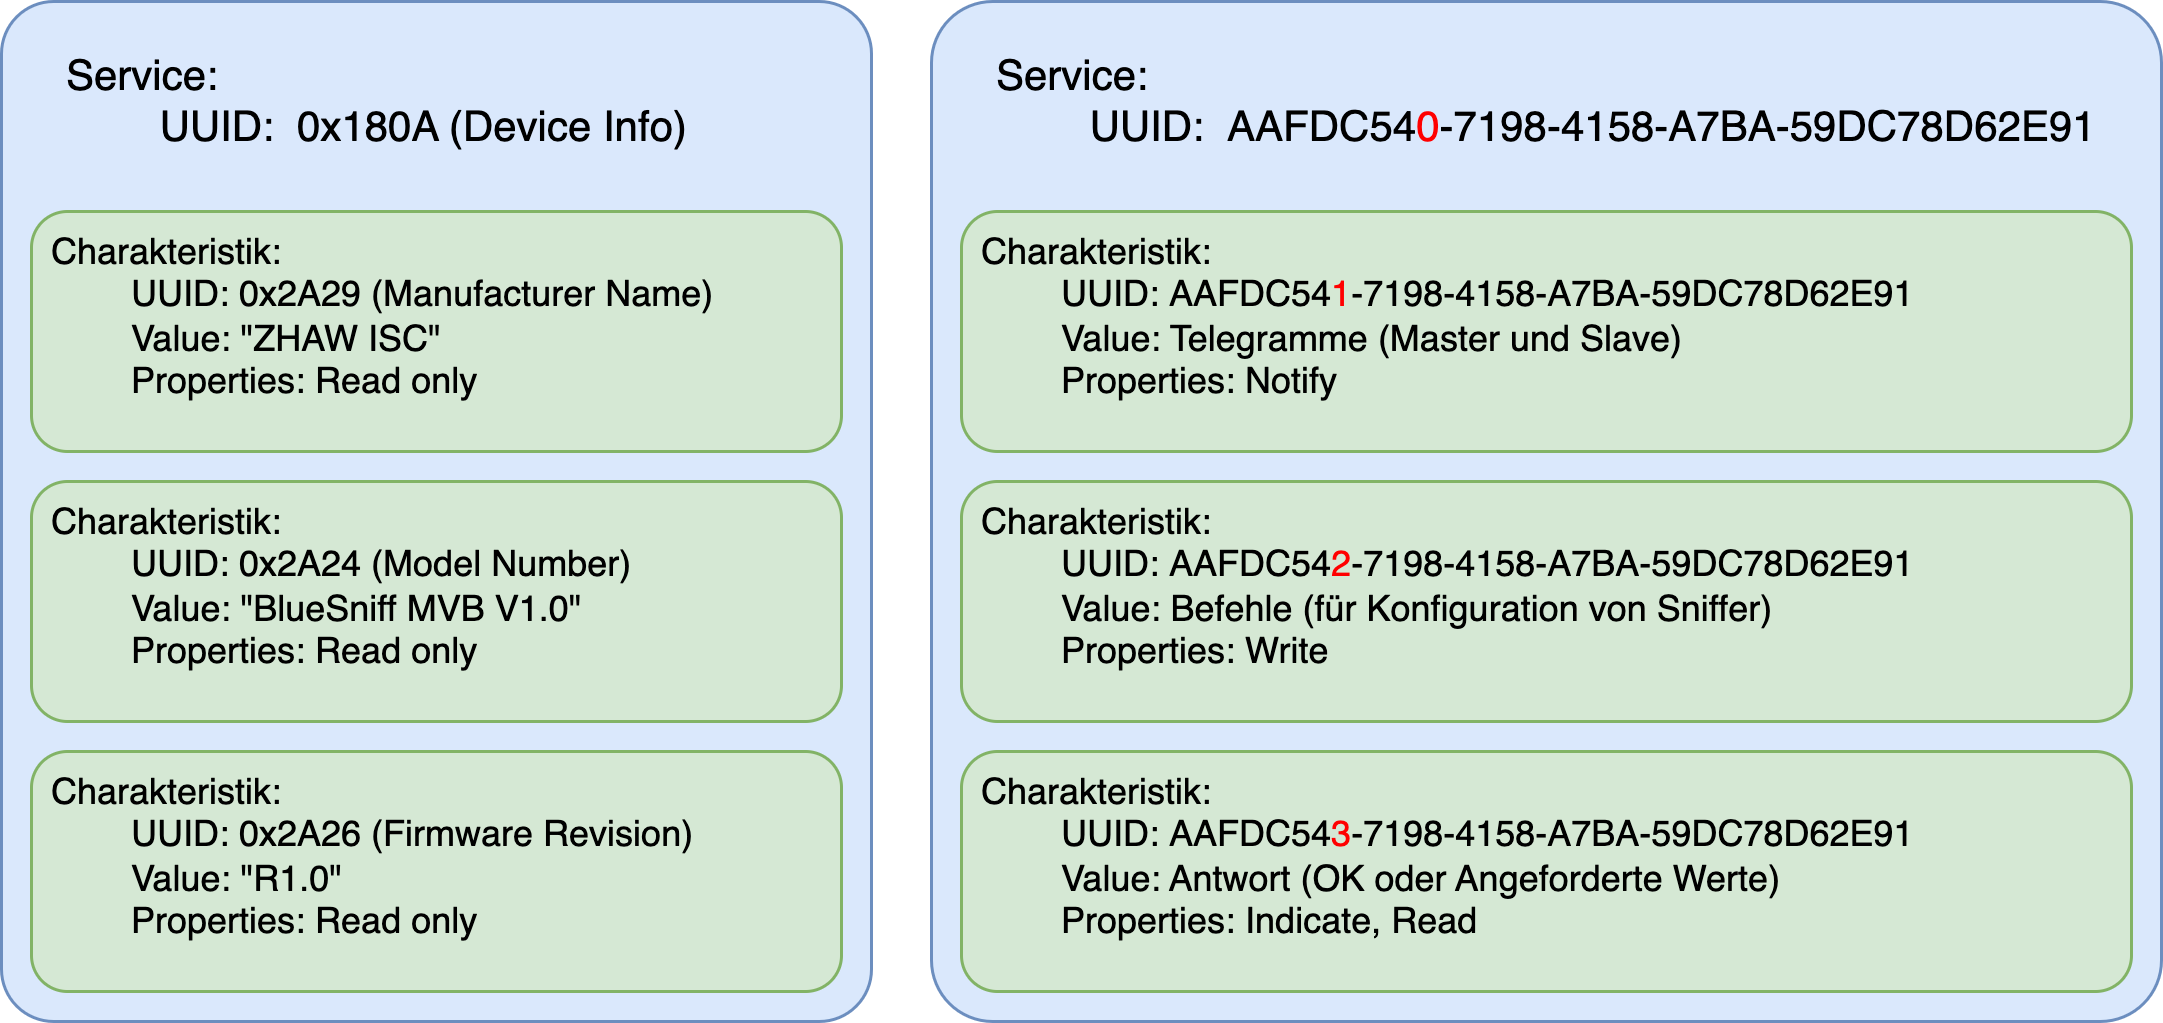
\includegraphics[width=0.9\linewidth]{Figures/Chap3/ESP/BLE/BLE.png}
    \caption{Bluetooth GATT Server auf ESP3-S3}
    \label{fig:BLEGATT}
\end{figure}

\subsubsection{Service - Device Info}
Der Service \textit{0x180A} zur \textit{Device Info} stellt dabei grundlegend statische Werte zur Verfügung, welche die Identifikation des Gerätes mit \textit{0x2A24 Model Number} oder die Aktualität der Firmware \textit{0x2A26 Firmware Revision} nach aussen zur Verfügung stellen. Die aktuellen Werte sind Beispielwerte und werden sich zu einem späteren Zeitpunkt ändern. 

\subsubsection{Service - Sniffer}
Der zweite Service stellt keine vordefinierte 16bit UUID zur Verfügung. Daher wurde diese Service-UUID mithilfe eines \textit{Online UUID Generator} generiert. In Abbildung \ref{fig:BLEGATT} ist die Zahl an 8. Stelle rot markiert. Dies soll darauf hinweisen, dass diese Zahl für die Charakteristiken inkrementiert wurde. Der selbstdefinierte Service soll den Datenaustausch zwischen Sniffer und Endgerät handeln. 

Die Charakteristik mit der roten Zahl 1 soll dabei die empfangenen Telegramme nach aussen schicken. Der erwartete Data-Throughput ist gemäss Kapitel \ref{tab:Busauslastung} bei Übertragung des gesamten MVB-Traffics hoch. Aus diesem Grund ist die \textit{Propertie} dieser Charakteristik auf \textbf{Notify} gesetzt.

Die Charakteristik mit der roten Zahl 2 soll ein individualisierbares Befehlsset schicken können, womit der Sniffer gesteuert, beziehungsweise dessen Verhalten geändert werden kann. Beispiele dazu sind die Einstellung eines Filters oder die Abfrage von Parametern (siehe dazu Kapitel \ref{sec:AusblickFirmwareESP32}). Weil die Befehle auf den Sniffer geschrieben werden, ist die \textit{Propiertie} in diesem Fall \textbf{Write}.

Die Charakteristik mit der roten Zahl 3 soll die Befehle, welche mit der vorherigen Charakteristik geschickt worden sind, mit einer OK-Message bestätigen oder einen Payload haben. Die \textit{Propiertie} ist auf \textbf{Indicate} gesetzt, sodass der Sniffer eine Rückmeldung schickt, sobald er diese bereit hat. Im Falle eines Timeouts kann das Endgerät auch einen \textbf{Read} auf die Charakteristik machen.



\subsection{Datenablage Code}
\label{sub:DatenablageCodeESP32S3}
Das gesamte Projektfile ist im Anhang \ref{app:Ordner41} beigefügt worden. Im Ordner "main" sind 3 Files ersichtlich, die hier kurz erläutert werden.
\begin{itemize}
    \item \textbf{Sniffer\_FW.c}: Das main() File mit dem Einstiegspunkt in der Funktion \textit{app\_main()}.
    \item \textbf{gatt\_svr.c}: Der selbst erstellte GATT-Server gemäss Kapitel \ref{sub:BluetoothGATT}.
    \item \textbf{gatt\_svr.h}: Das Header File zu gatt\_svr.c
\end{itemize}

Das File "'sdkconfig"' entspricht der aktuellen Konfiguration des Projektes. Dort sind beispielsweise die NimBle-Einstellungen ersichtlich und können geändert werden. 

%----------------------------------------------------------------------
% SECTION Hardware PCB
%----------------------------------------------------------------------
\section{Hardware Design}
\label{sec:Hardware Design}

In diesem Unterkapitel wird die Entwicklung der Hardware für den MVB-Sniffer beschrieben. Zu den Kernkomponenten zählen der RS485-Transceiver SP3485CN-L/TR, das FPGA 10M08SAE144C8G und der Mikrocontroller ESP32-S3-WROOM-1. Die Hauptaufgabe besteht darin, die Funktionalitäten der drei Evaluationsboards zu analysieren und die Bauteile auf die für die Anwendung als MVB-Sniffer notwendigen Komponenten zu reduzieren. Dabei wurde auch berücksichtigt, welche zusätzlichen Funktionen in der weiteren Entwicklung von Nutzen sein könnten. Ziel ist, ein für den Anwendungszweck optimiertes PCB-Design (Printed Circuit Board) zu erstellen, das alle wesentlichen Anforderungen für die Signalverarbeitung und -analyse erfüllt und die verschiedenen elektronischen Bauteile und Chips in einem kompakten Design vereint. Im Rahmen dieser Arbeit wurde zunächst ein Schema erstellt, welches als Grundlage für die spätere Entwicklung des PCB dient. Als Software wurde hierfür Altium verwendet. Die Abbildung \ref{fig:Hardware Übersicht} zeigt ein vereinfachtes Blockschaltbild, wie die Komponenten zusammen verbunden sind. Das System wird per Micro USB mit Spannung versorgt und besitzt über 3 DC/DC-Wandler. Für das FPGA  ein Wandler von 5 V auf 3.3 V, für den ESP32-S3 und den RS485 ebenfalls ein Wandler von 5 V auf 3.3 V und für die Referenzspannung des FPGA ein Wandler von 3.3 V auf 2.5 V. Nachfolgend werden die zentralen Funktionen anhand von Ausschnitten aus dem Schema detailliert erläutert. Das gesamte Schema ist in PDF-Format im Anhang \ref{app:Schemata} aufzufinden, sowie die Stückliste dazu \ref{app:bom.pdf}.

\begin{figure}[H]
    \centering
    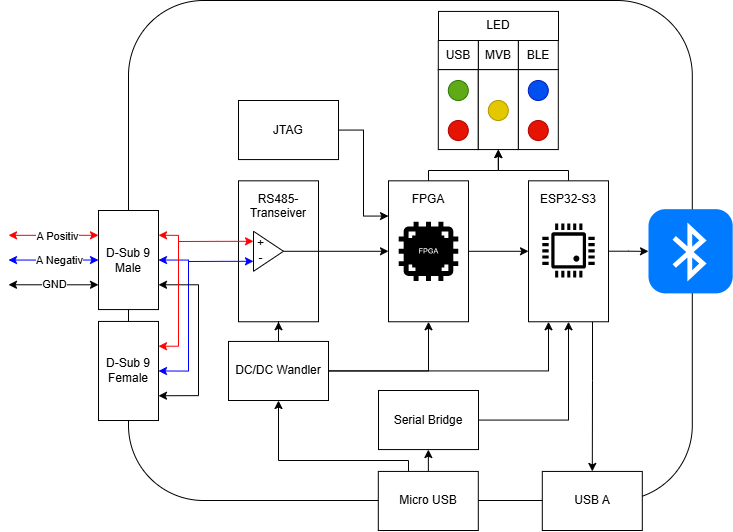
\includegraphics[width=0.8\linewidth]{Figures/Chap3/Schematics/Aufbau_Hardware_Sniffer.drawio.png}
    \caption{Hardware Übersicht}
    \label{fig:Hardware Übersicht}
\end{figure}


\subsection{RS485-Transceiver}

Wie in Abbildung \ref{fig:MVB to RS485} ersichtlich, wird das MVB-Signal durch den Sniffer über die beiden D-Sub-Stecker J1 und J2 durchgeführt und abgegriffen. Anschliessend wird es zum RS485-Transceiver SP3485CN-L/TR weitergeleitet. Der RS485-Transceiver verarbeitet die differentiellen Signale des MVB \textit{Data P} und \textit{Data N}. Er wandelt diese in ein einheitliches Signal \textit{MVB Data} um, das für die Weiterverarbeitung durch den FPGA verwendet wird. Dabei werden lediglich die 3 Leitungen der Linie A des MVB-Signals analysiert, während die redundante Linie B nicht abgegriffen wird (Pin 4 und Pin 5 des D-Sub-Steckers), da sie in Fahrzeugen in der Praxis selten verwendet wird. Die Pins \textit{DI}, $\overline{RE}$ und \textit{DE} werden mit dem \textit{GND} gelegt, um sicherzustellen, dass der Sniffer nur als Empfänger fungiert. Durch diese Konfiguration ist der Treiber deaktiviert (\textit{DE} auf \textit{GND}) und der Empfänger aktiviert ($\overline{RE}$ auf \textit{GND}), sodass das Gerät nur Daten vom MVB empfangen kann, ohne selbst Daten auf den Bus zu senden. Dies verhindert, dass der Datenverkehr auf dem Bus unbeabsichtigt beeinflusst wird. Die weiteren Pin Funktionen sind aus der Tabelle \ref{tab:pin_funktionen} zu entnehmen. Das Datenblatt befindet sich im Anhang \ref{app:File51}.

\begin{figure}[H]
    \centering
    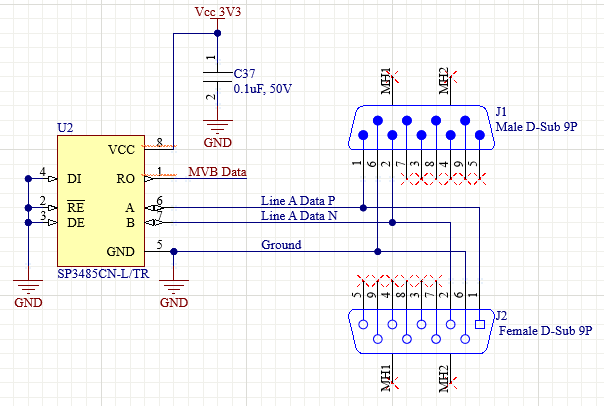
\includegraphics[width=0.8\linewidth]{Figures/Chap3/Schematics/MVB to RS485.png}
    \caption{Vom MVB Signal zum RS485}
    \label{fig:MVB to RS485}
\end{figure}

\begin{table}[h]
  \centering
  \begin{tabular}{|c|c|l|}
    \hline
    \textbf{Pin} & \textbf{Funktion} & \textbf{Beschreibung} \\ \hline
    1 & RO & Receiver Output \\ \hline
    2 & $\overline{\text{RE}}$ & Receiver Output Enable Active LOW \\ \hline
    3 & DE & Driver Output Enable \\ \hline
    4 & DI & Driver Input \\ \hline
    5 & GND & Ground Connection \\ \hline
    6 & A & Driver Output/Receiver Input Non-inverting \\ \hline
    7 & B & Driver Output/Receiver Input Inverting\\ \hline
    8 & Vcc & Versorgungsspannung \\ \hline
  \end{tabular}
  \caption{Beschreibung der Pin-Funktionen}
  \label{tab:pin_funktionen}
\end{table}

\textcolor{red}{Datenblatt SP3485CN-L/TR} 

\subsection{FPGA}
Ein FPGA ist ein flexibler Chip, der aus programmierbaren Logikblöcken, I/O-Banken und Verbindungsnetzwerken besteht. Die Konfiguration entscheidet, welche Funktionen der FPGA übernimmt und wie die einzelnen Blöcke und Schnittstellen zusammenarbeiten. Der 10M08SAE144C8G verfügt über 8 Banken, die unterschiedlich konfiguriert werden können. Für die Anwendung im MVB-Sniffer wurde nur die Hälfte der Banken verwendet, jedoch alle 8 Banken mit Spannung versorgt, um für die Weiterentwicklung flexibel zu sein und um Störungen oder unerwartetes Verhalten zu vermeiden. 

\subsubsection{Programmierung}

Programmiert wird der FPGA über die JTAG-Schnittstelle (Joint Test Action Group). Das ist ein standardisiertes Protokoll zur Programmierung, Konfiguration und Debuggen von elektronischen Bausteinen wie Mikrocontrollern oder FPGA. Über die JTAG-Signale \textit{TCK} (Test Clock), \textit{TMS} (Test Mode Select), \textit{TDI} (Test Data Input) und \textit{TDO} (Test Data Output) können Daten seriell übertragen werden. Das Signal \textit{JTAGEN} (JTAG Enable) aktiviert die JTAG-Funktion. Im FPGA wird die Bank 1B für die JTAG-Schnittstelle verwendet, die eine zentrale Rolle bei der Konfiguration des FPGA spielt. Dies konnte vom Evaluationsboard übernommen werden, da dieses so programmiert wird. Es sind zwei Modi möglich:

\begin{enumerate}
    \item Direkte Konfiguration über .sof-Dateien:
    Mithilfe des JTAG-Steckers kann eine .sof-Datei direkt in das FPGA geladen werden. Diese Datei enthält die Informationen für die momentane Programmierung des FPGA. Dabei wird der FPGA bei einem Neustart oder einer erneuten Konfiguration in einen leeren Zustand versetzt, da die Konfiguration nur temporär gespeichert wird.
    \item Programmierung der Configuration Flash Memory (CFM) mit .pof-Dateien: 
    Alternativ kann über den JTAG-Header eine .pof-Datei in das CFM des FPGA programmiert werden. In diesem Fall startet der FPGA nach jedem Neustart automatisch in den Selbstkonfigurationsmodus und lädt die gespeicherten Daten aus dem CFM.
\end{enumerate}

\begin{figure}[H]
    \centering
    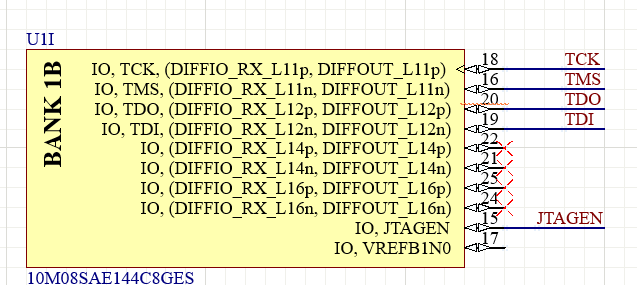
\includegraphics[width=1.0\linewidth]{Figures/Chap3/Schematics/Bank1B_JTAG.png}
    \caption{FPGA Bank 1B: JTAG}
    \label{FPGA JTAG}
\end{figure}

Wie in Abbildung \ref{FPGA JTAG} ersichtlich, ist die JTAG-Schnittstelle der Stecker \textit{J6}, welche mit einem USB-Blaster verbunden werden kann. Die 10 kOhm Widerstände sorgen dafür, dass die Signale \textit{TCK}, \textit{TMS} und \textit{JTAGEN} auf logisch \textit{"1"} gehalten werden, wenn sie nicht aktiv angesteuert werden. Dies verhindert Fehlfunktionen durch unbestimmte Pegel. Der 1 kOhm Widerstand hält \textit{TDI} auf logisch \textit{"0"}, wenn kein Signal anliegt, auch um ungewollte Signalpegel zu vermeiden. Somit werden die Signale über die Pins des Steckers \textit{J6} mit dem FPGA verbunden, \textit{JTAGEN} wird auf logisch \textit{"1"} gezogen, wodurch das FPGA in den Programmierungsmodus versetzt wird und über die restlichen Pins die Programmdaten und Steuersignale an das FPGA sendet.


\subsubsection{Oszillator}

Es wird analog zum Evaluationsboard der Oszillator CB3LV-3C-50M0000 verwendet, damit ein stabiler und präziser externer Takt von 50 MHz zur Verfügung steht. Dieser Takt wird benötigt, um die Abläufe im FPGA zu synchronisieren und zusätzliche Takte zu erzeugen, die es für bestimmte Aufgaben braucht. Dafür wird der Oszillator mit einem dedizierten Clock-Pin des FPGA auf Bank 2 verbunden (siehe Abbildung \ref{FPGA OSC}).

\begin{figure}[H]
    \centering
    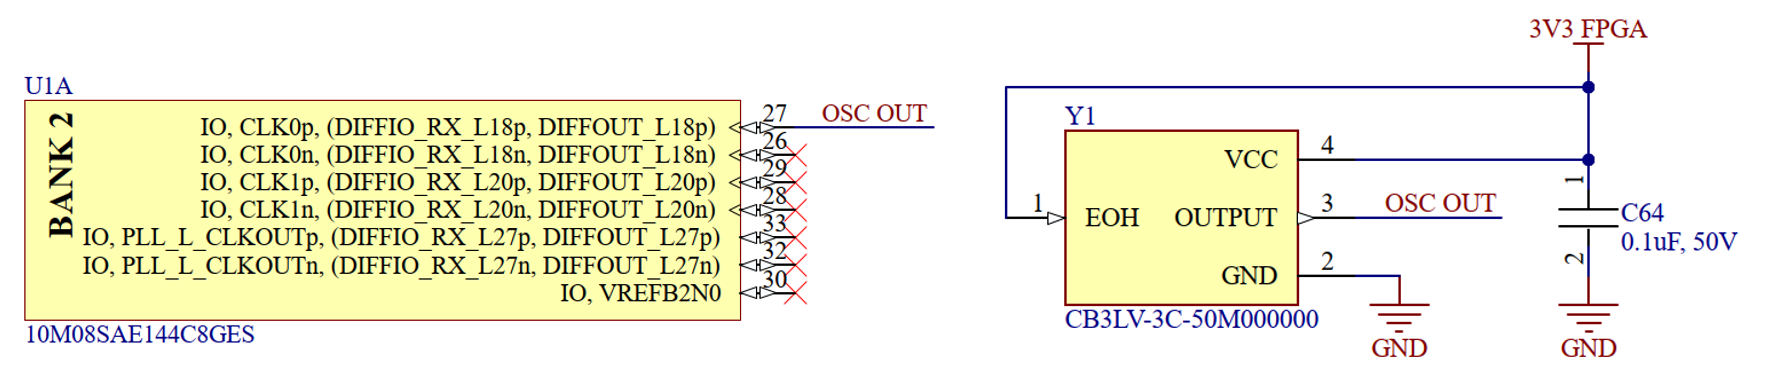
\includegraphics[width=1.0\linewidth]{Figures/Chap3/Schematics/Bank2_OSC.png}
    \caption{FPGA Bank 2: Oszillator}
    \label{FPGA OSC}
\end{figure}

\subsubsection{Steuersignale}
\label{subsec:Steuersignale}

Auf der Bank 8 des FPGA gibt es mehrere Steuersignale, die in der zukünftigen Anwendung von wichtiger Bedeutung sein können (siehe Abbildung \ref{FPGA Admin}).

\begin{itemize}
    \item Durch das Betätigen des Knopfes S4 wird das FPGA gezwungen, sich aus dem Configuration Flash Memory (CFM) neu zu konfigurieren, indem das \textit{NCONFIG} Signal vom FPGA auf das \textit{GND} Potenzial gezogen wird. Da in Zukunft die Programmierung über die CFM laufen soll, erscheint diese Funktion als wichtig.
    
    \item Das Betätigen des Knopfes S4 setzt alle Register im FPGA zurück. Dies kann für eine schnelle Rücksetzung des Systems genutzt werden, ohne das FPGA vollständig neu zu konfigurieren. Das Signal \textit{RESET N} wird auf den dafür vorgesehenen Pin auf dem FPGA geführt und beim Drücken vom Knopf S4 auf das \textit{GND} Potenzial gezogen.
    
    \item Mit diesem Schalter SW1 wird ausgewählt, welches CFM-Bild (Konfigurationsbild) beim Start des FPGA verwendet wird, wenn eine Dual-Image-Konfiguration vorliegt. Diese Funktionen ermöglichen eine flexible Konfiguration und Steuerung des FPGA, insbesondere wenn in einem zukünftigen Schritt mehrere Konfigurationsoptionen gefordert werden, wie zum Beispiel eine Umschaltung von ESD auf EMD. Dies geschieht mit dem Steuersignal \textit{BOOT SEL}.
\end{itemize}

\begin{figure}[H]
    \centering
    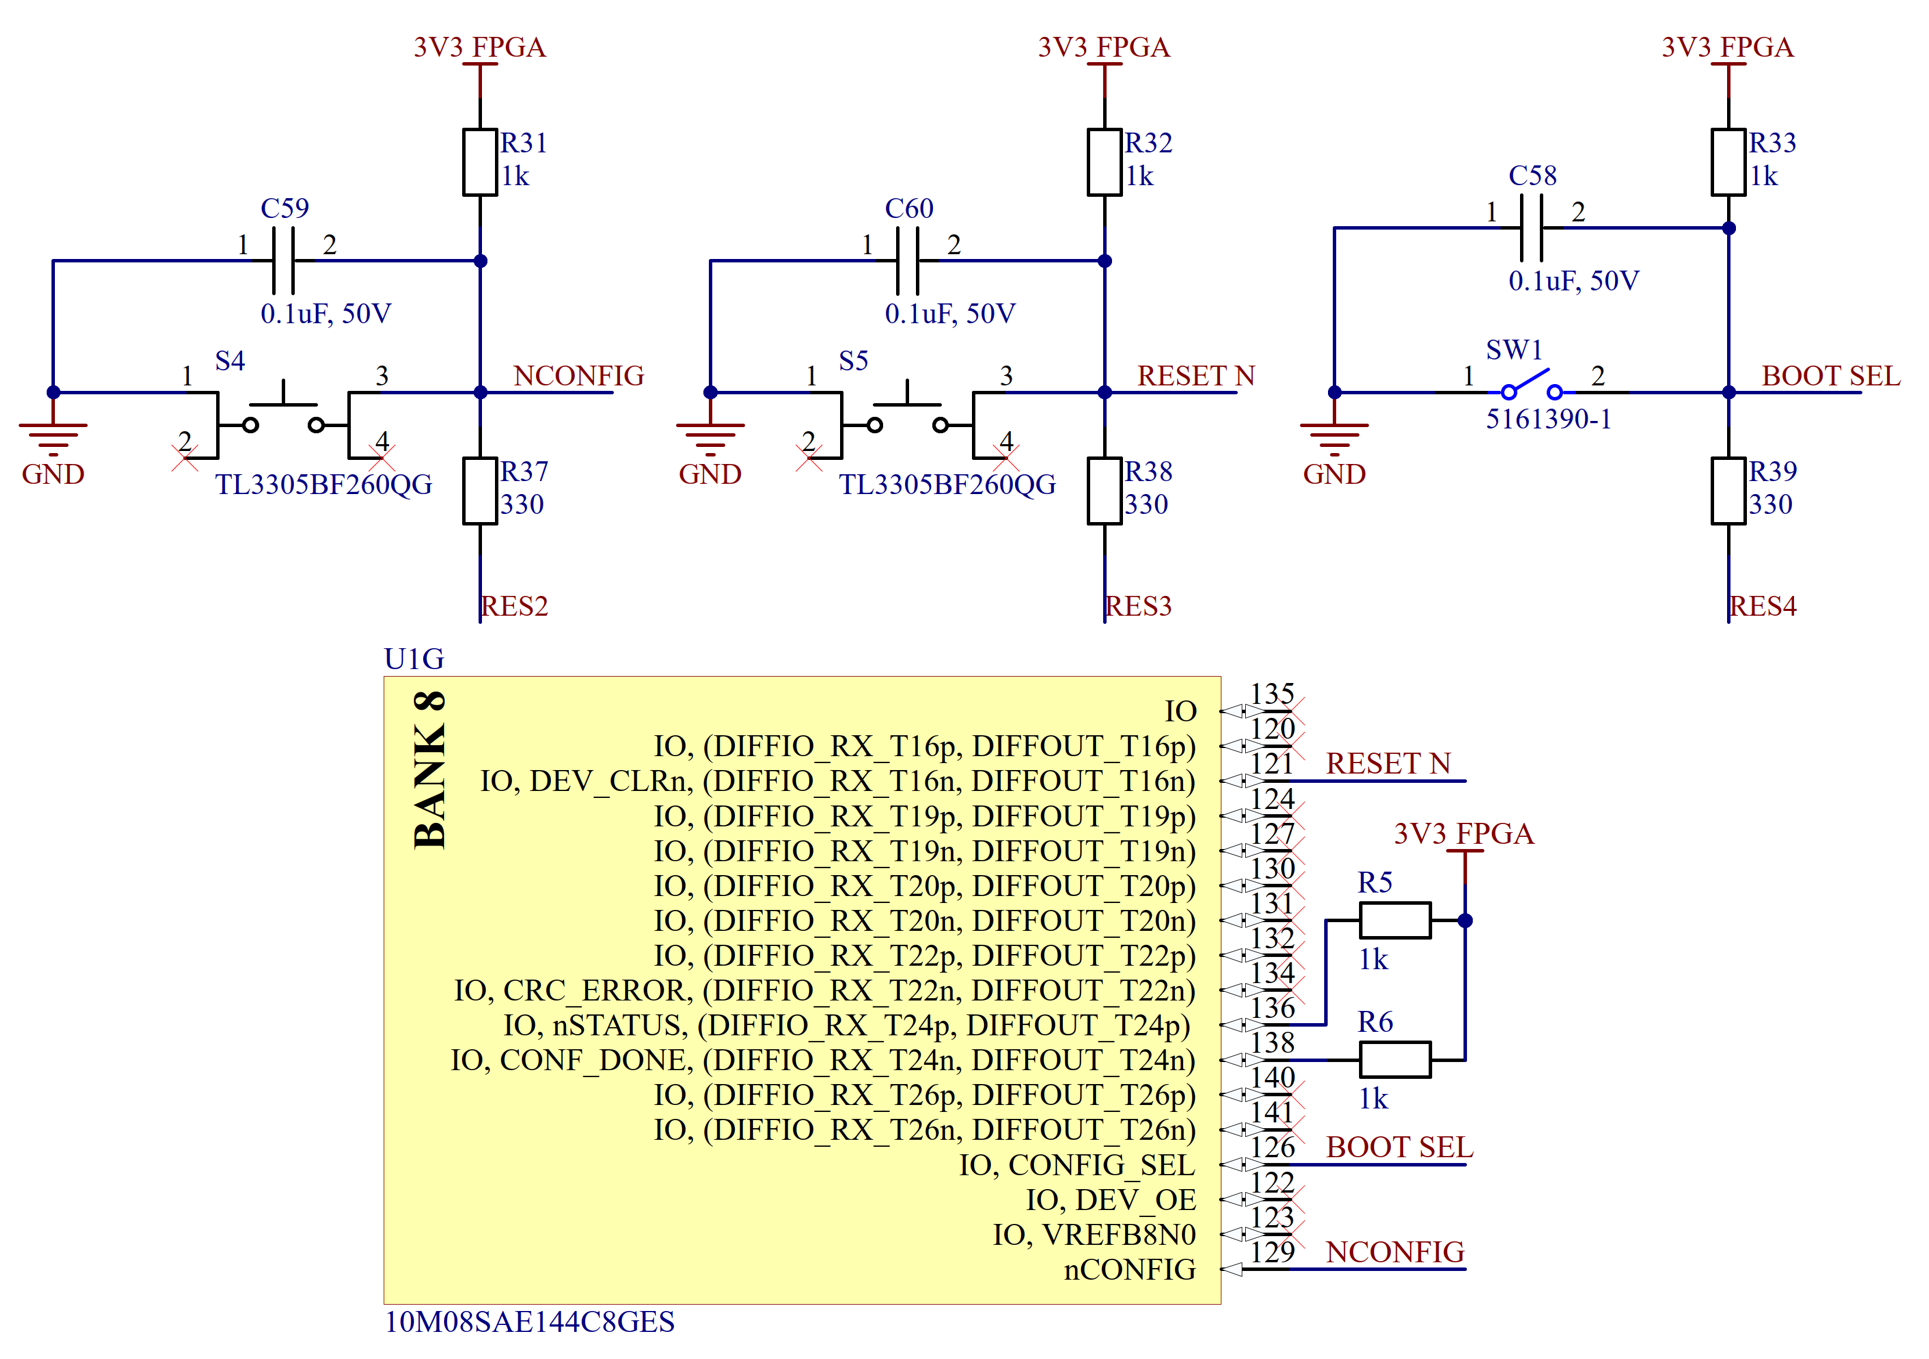
\includegraphics[width=1.0\linewidth]{Figures/Chap3/Schematics/Bank8_Admin.png}
    \caption{FPGA Bank 8: Steuersignale FPGA}
    \label{FPGA Admin}
\end{figure}

Diese drei Steuersignale können auch über die \textit{RES2} bis \textit{RES4} Leitungen vom Mikro Controller ESP32-S3 gesteuert werden. Dies geschieht über die Pull-Down-Widerstände R33 bis R35 und den entsprechenden GPIO vom ESP32, welche die Leitungen auf logisch \textit{"0"} ziehen können.

\subsubsection{Schnittstellen}
\label{subsubsec:Schnittstellen}
Für die Kommunikation zwischen dem FPGA, dem ESP32-S3 und dem RS485 wurde die Bank 3 vorgesehen. In dieser Bank sind die SPI-Signale (\textit{CS, MOSI} und \textit{SCLK}) so verbunden, dass eine direkte Kommunikation zwischen dem FPGA und dem ESP32-S3 ermöglicht wird. Um die Überschwinger zu reduzieren, wurden bereits 0 Ohm Widerstände angedacht, die in Zukunft ersetzt werden können durch grössere Widerstände. Zusätzlich wurde eine Handshake-Leitung \textit{HS FPGA}, Interrupt-Leitung \textit{INTR FPGA} und eine Master In, Slave Out Leitung \textit{MISO} integriert, um künftige Erweiterungen zu vereinfachen.

Darüber hinaus stehen die Reserveleitungen \textit{RES1} bis \textit{RES4} zur Verfügung. Diese Leitungen können neben der Funktion, den FPGA zu steuern, wie im letzten Abschnitt von Kapitel \ref{subsec:Steuersignale}(\textit{RES2} bis \textit{RES4}) beschrieben, auch als zusätzliche Verbindung zwischen FPGA und ESP32-S3 dienen, wo sie noch keine festgelegte Funktion besitzen.

Zusätzlich wurden \textit{FPGA RES5} bis \textit{FPGA RES7} Leitungen angedacht, welche direkt auf eine Pinleiste gehen. Somit kann über einen Steckverbinder künftig die FPGA IO, flexibel und schnell erweitert werden.

Für das Signal \textit{MVB Active} wurde eine LED-Ansteuerung mithilfe eines Darlington-Arrays vorgesehen (Details dazu in Kapitel \ref{subsec:Indikatoren}). Somit soll der Sniffer in Zukunft anzeigen, sobald er MVB Aktivität auf dem RS485 erkennt.

\begin{figure}[H]
    \centering
    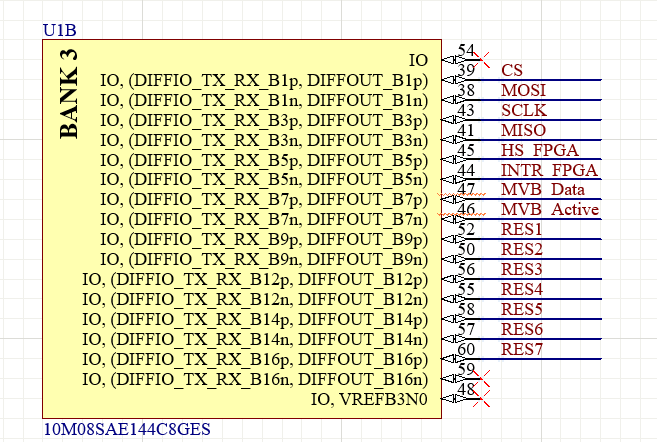
\includegraphics[width=1.0\linewidth]{Figures/Chap3/Schematics/Bank3_ESP.png}
    \caption{FPGA Bank 3: ESP32 Interface}
    \label{FPGA ESP}
\end{figure}

Das Datenblatt sowie das Schema des FPGA Evaluationsboards befinden sich im Anhang \ref{app:File52} (Datenblatt) und \ref{app:File53} (Schema).

\subsection{ESP32-S3}
Der Mikrocontroller ESP32-S3-WROOM-1 unterstützt Bluetooth Low Energy (BLE), WLAN, verfügt über eine hohe Flexibilität bei der Konfiguration der GPIO, einen Dual-Core-Prozessor und bietet eine Vielzahl von Schnittstellen wie SPI, I$^2$C und UART.

\subsubsection{Programmierung}
Die USB-UART-Brücke CP2102N-A02-GQFN28, in Abbildung \ref{fig:UART_Bridge}, ermöglicht die einfache Kommunikation zwischen einem Computer und dem ESP32-S3 Mikrocontroller über die serielle Schnittstelle. Diese UART-Verbindung wird vor allem für das Flashen der Firmware auf den ESP32, sowie für Debugging-Zwecke genutzt. Die Leitungen \textit{USB DP} und \textit{USB DN} kommen von einer Micro-USB-Schnittstelle auf den CP2102N. Von dort gehen die Leitungen \textit{U0RXD} und \textit{U0TXD} dann weiter zum ESP32.

Eine Programmierschaltung ermöglicht eine automatische Umschaltung des ESP32-S3 zwischen Normalmodus (Run) und Programmiermodus (Boot), ohne dass physische Tasten erforderlich sind. Mit dem CP2102N und dessen Steuerleitungen \textit{DTR, RTS} kann der ESP32-S3 in die verschiedenen Modi geschaltet werden. Über eine Transistorschaltung werden diese Leitungen verwendet, um die Pins EN (Reset) und GPIO0 (Boot-Modus) auf dem ESP32-S3 anzusteuern, wie in Abbildung \ref{fig:ESP32_Steuersignale} ersichtlich. Das Gleiche kann auch über die Taster S1 und S2 gemacht werden und der S3 besitzt noch keine Funktion, kann in Zukunft aber beliebig verwendet werden.

\begin{figure}[H]
    \centering
    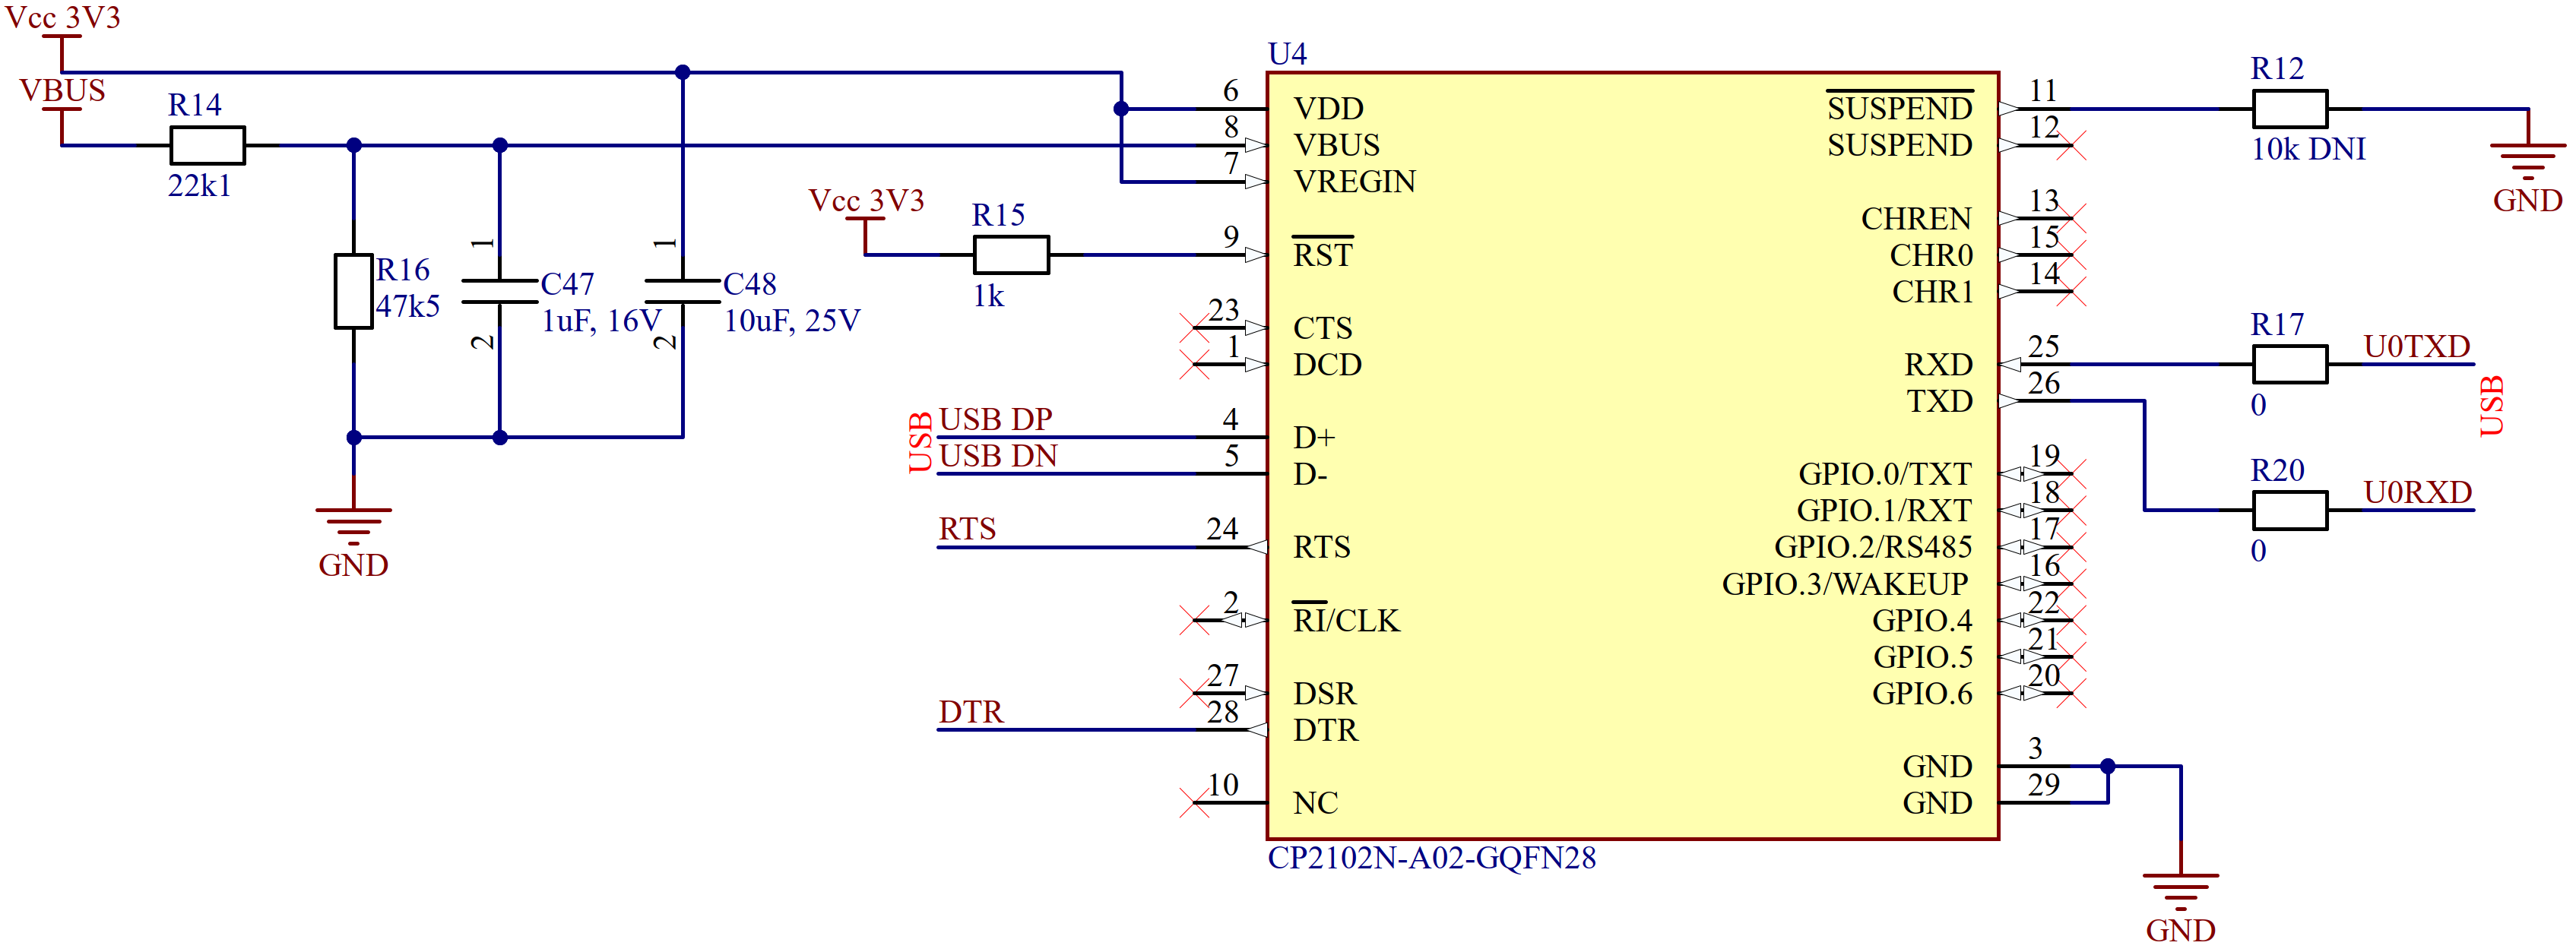
\includegraphics[width=1\linewidth]{Figures/Chap3/Schematics/UART_Bridge.png}
    \caption{USB-UART-Brücke}
    \label{fig:UART_Bridge}
\end{figure}

Das Datenblatt der USB-UART-Brücke CP2102N-A02 befindet sich im Anhang \ref{app:File54}.

\begin{figure}[H]
    \centering
    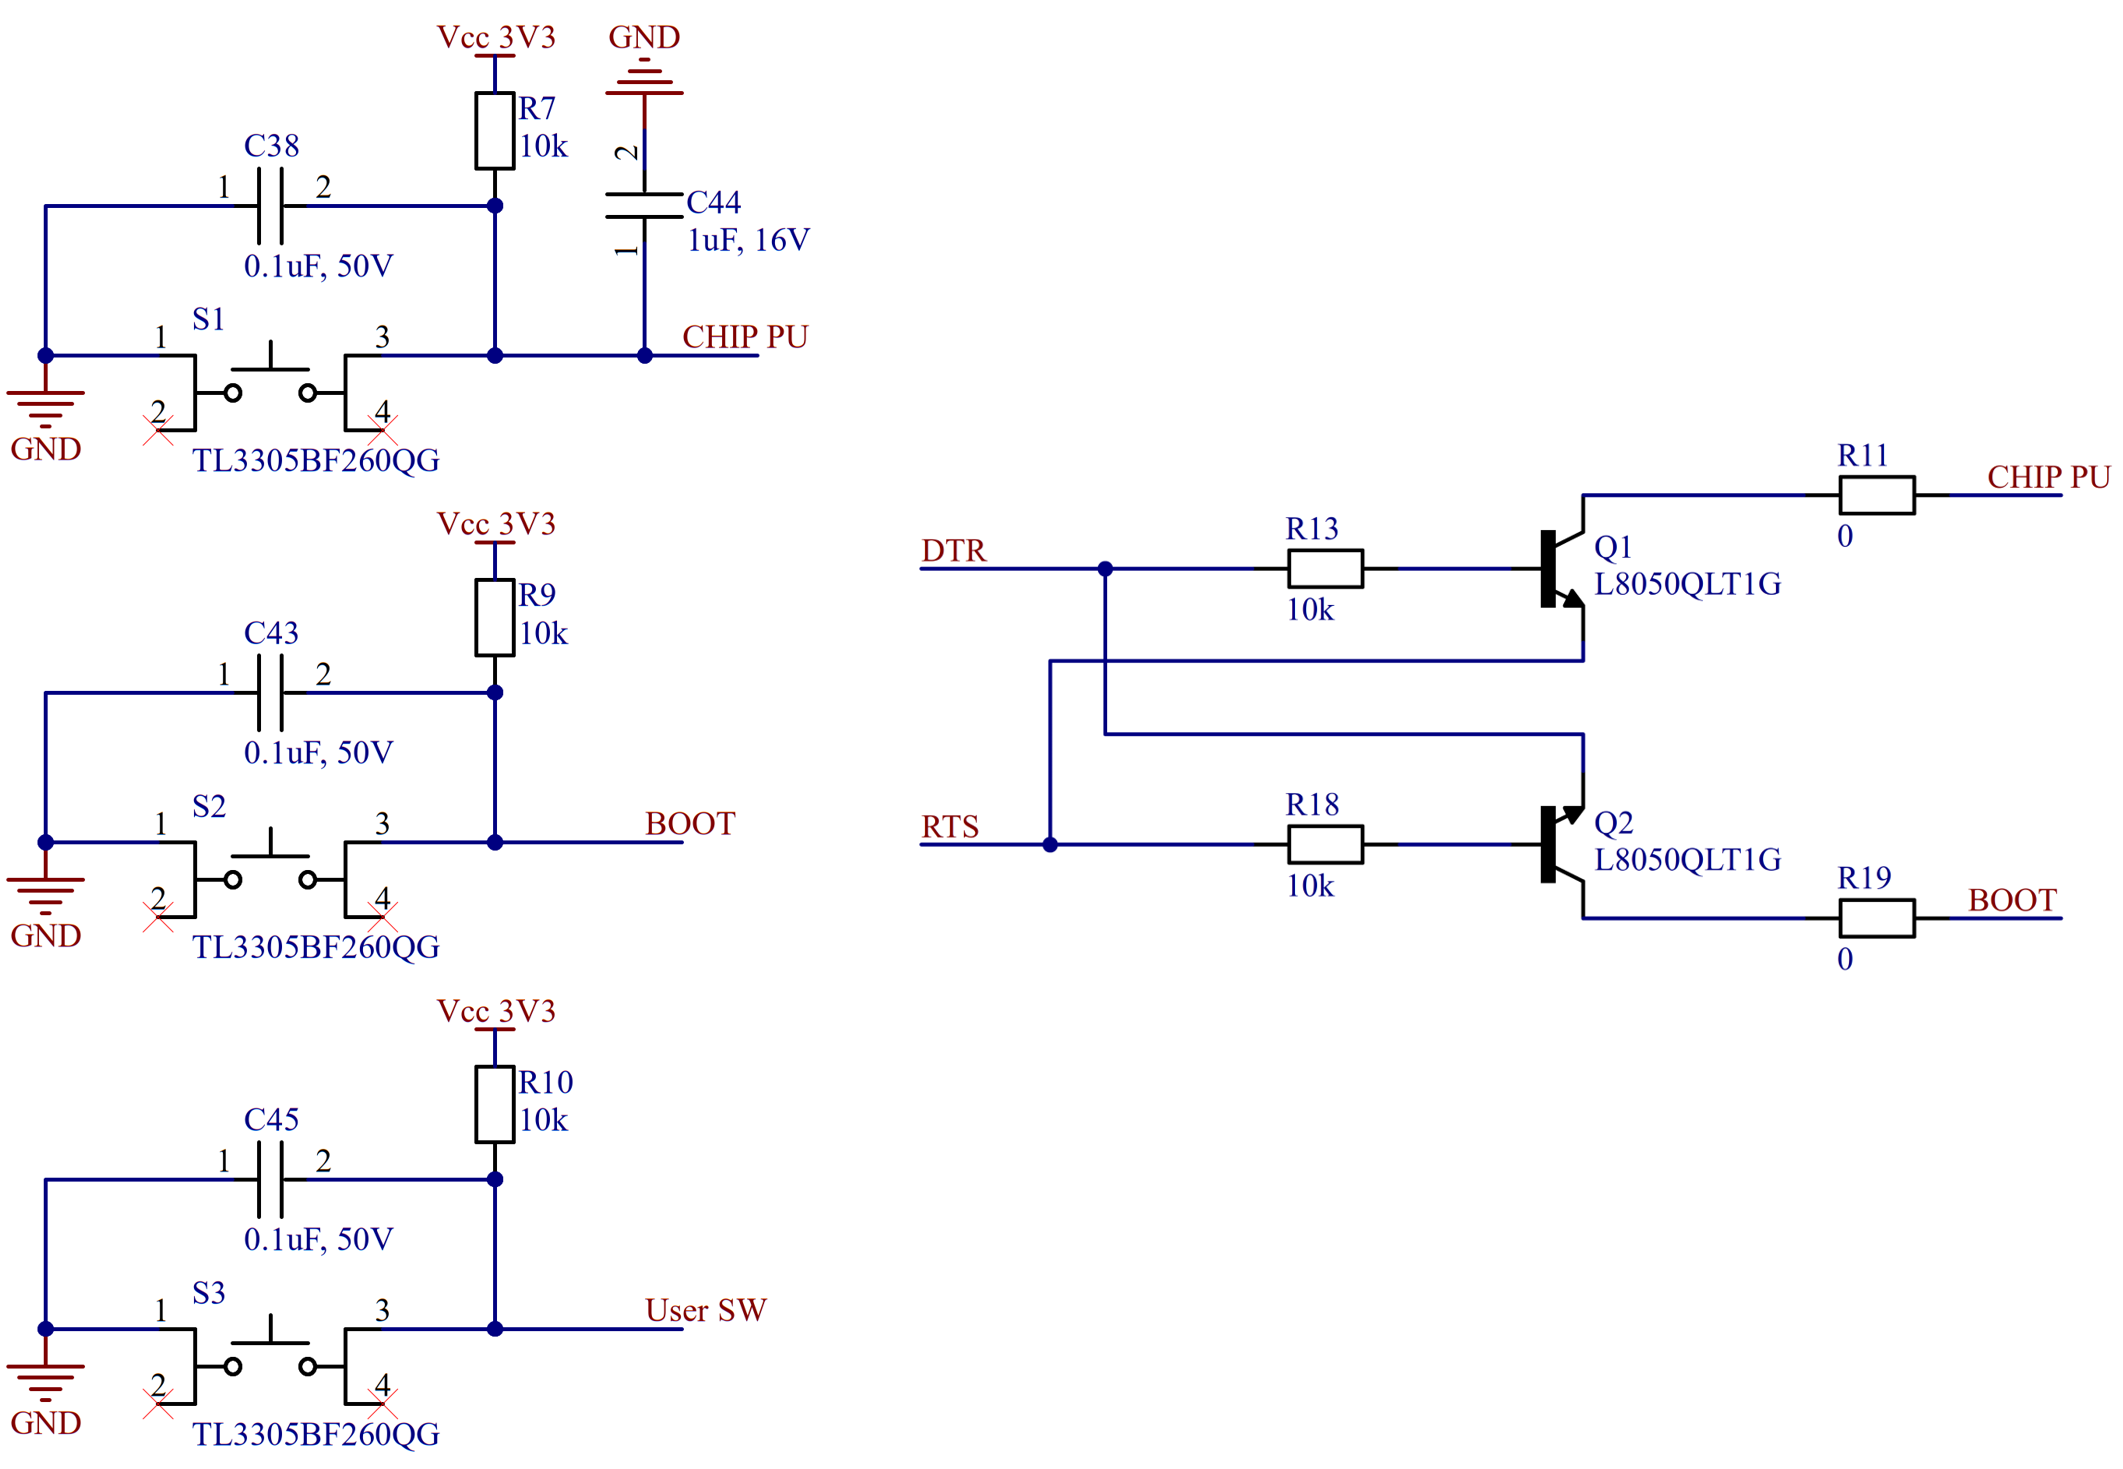
\includegraphics[width=1\linewidth]{Figures/Chap3/Schematics/ESP32_Steuersignale.png}
    \caption{ESP32 Steuersignale}
    \label{fig:ESP32_Steuersignale}
\end{figure}

Normalbetrieb
\textit{DTR} = 1, \textit{RTS} = 1: Beide Transistoren bleiben gesperrt, wodurch EN und GPIO0 auf HIGH liegen. Der ESP32-S3 startet und läuft im Normalmodus.

Programmiermodus:
\textit{DTR} = 0, \textit{RTS} = 1: Der Transistor für GPIO0 (Boot-Pin) wird aktiviert, wodurch GPIO0 auf Low gezogen wird, während EN HIGH bleibt. Der ESP32-S3 wird dadurch in den Flash-Modus versetzt.

Reset:
\textit{DTR} = 1, \textit{RTS} = 0: Der Transistor für EN wird aktiviert, wodurch der Reset-Pin des ESP32-S3 (CHIP PU) auf Low gezogen wird. Dies führt zu einem Neustart des Mikrocontrollers. 

Diese Steuersignale wurden  zusammengefasst in der Tabelle \ref{tab:operation_modes}.
\begin{table}[h]
  \centering
  \begin{tabular}{|c|c|c|c|l|}
    \hline
    DTR & RTS & EN (CHIP PU) & GPIO0 & Modus \\ \hline
    1   & 1   & 1            & 1     & Normalbetrieb (Run) \\ \hline
    0   & 1   & 1            & 0     & Programmiermodus (Boot) \\ \hline
    1   & 0   & 0            & 1     & Reset \\ \hline
  \end{tabular}
  \caption{Operation Modi}
  \label{tab:operation_modes}
\end{table}



\subsubsection{USB-A}
Eine USB-A-Schnittstelle soll ermöglichen, in Zukunft Daten des Sniffers nicht nur per Bluetooth auszugeben, sondern auch über einen USB-Stick zu loggen, sodass man nicht immer mit einem Bluetooth-fähigen Gerät in der Nähe sein muss. Dies geschieht über zwei GPIO des ESP32. Die beiden Leitungen (\textit{USB-A N, USB-A P}) sind direkt mit dem ESP32-S3 verbunden und sind ersichtlich in Abbildung \ref{fig:ESP32}.

\subsubsection{GPIO}
 Die restlichen GPIO des ESP32-S3 in der Abbildung \ref{fig:ESP32} auf die noch nicht eingegangen worden ist, sind zum einen die 7 Leitungen, die LED ansteuern (\textit{BLE LED b, BLE LED r, USB LED g, USB LED r, Akku low, Akku mid, Akku full}). Hierzu folgt mehr in Kapitel \ref{subsec:Indikatoren}. Die Leitung \textit{ADC Akku} wird über einen Spannungsteiler auf dem ADC-Eingang vom ESP32-S3 eingelesen, um den Akkustand zu bestimmen.
 
\begin{figure}[H]
    \centering
    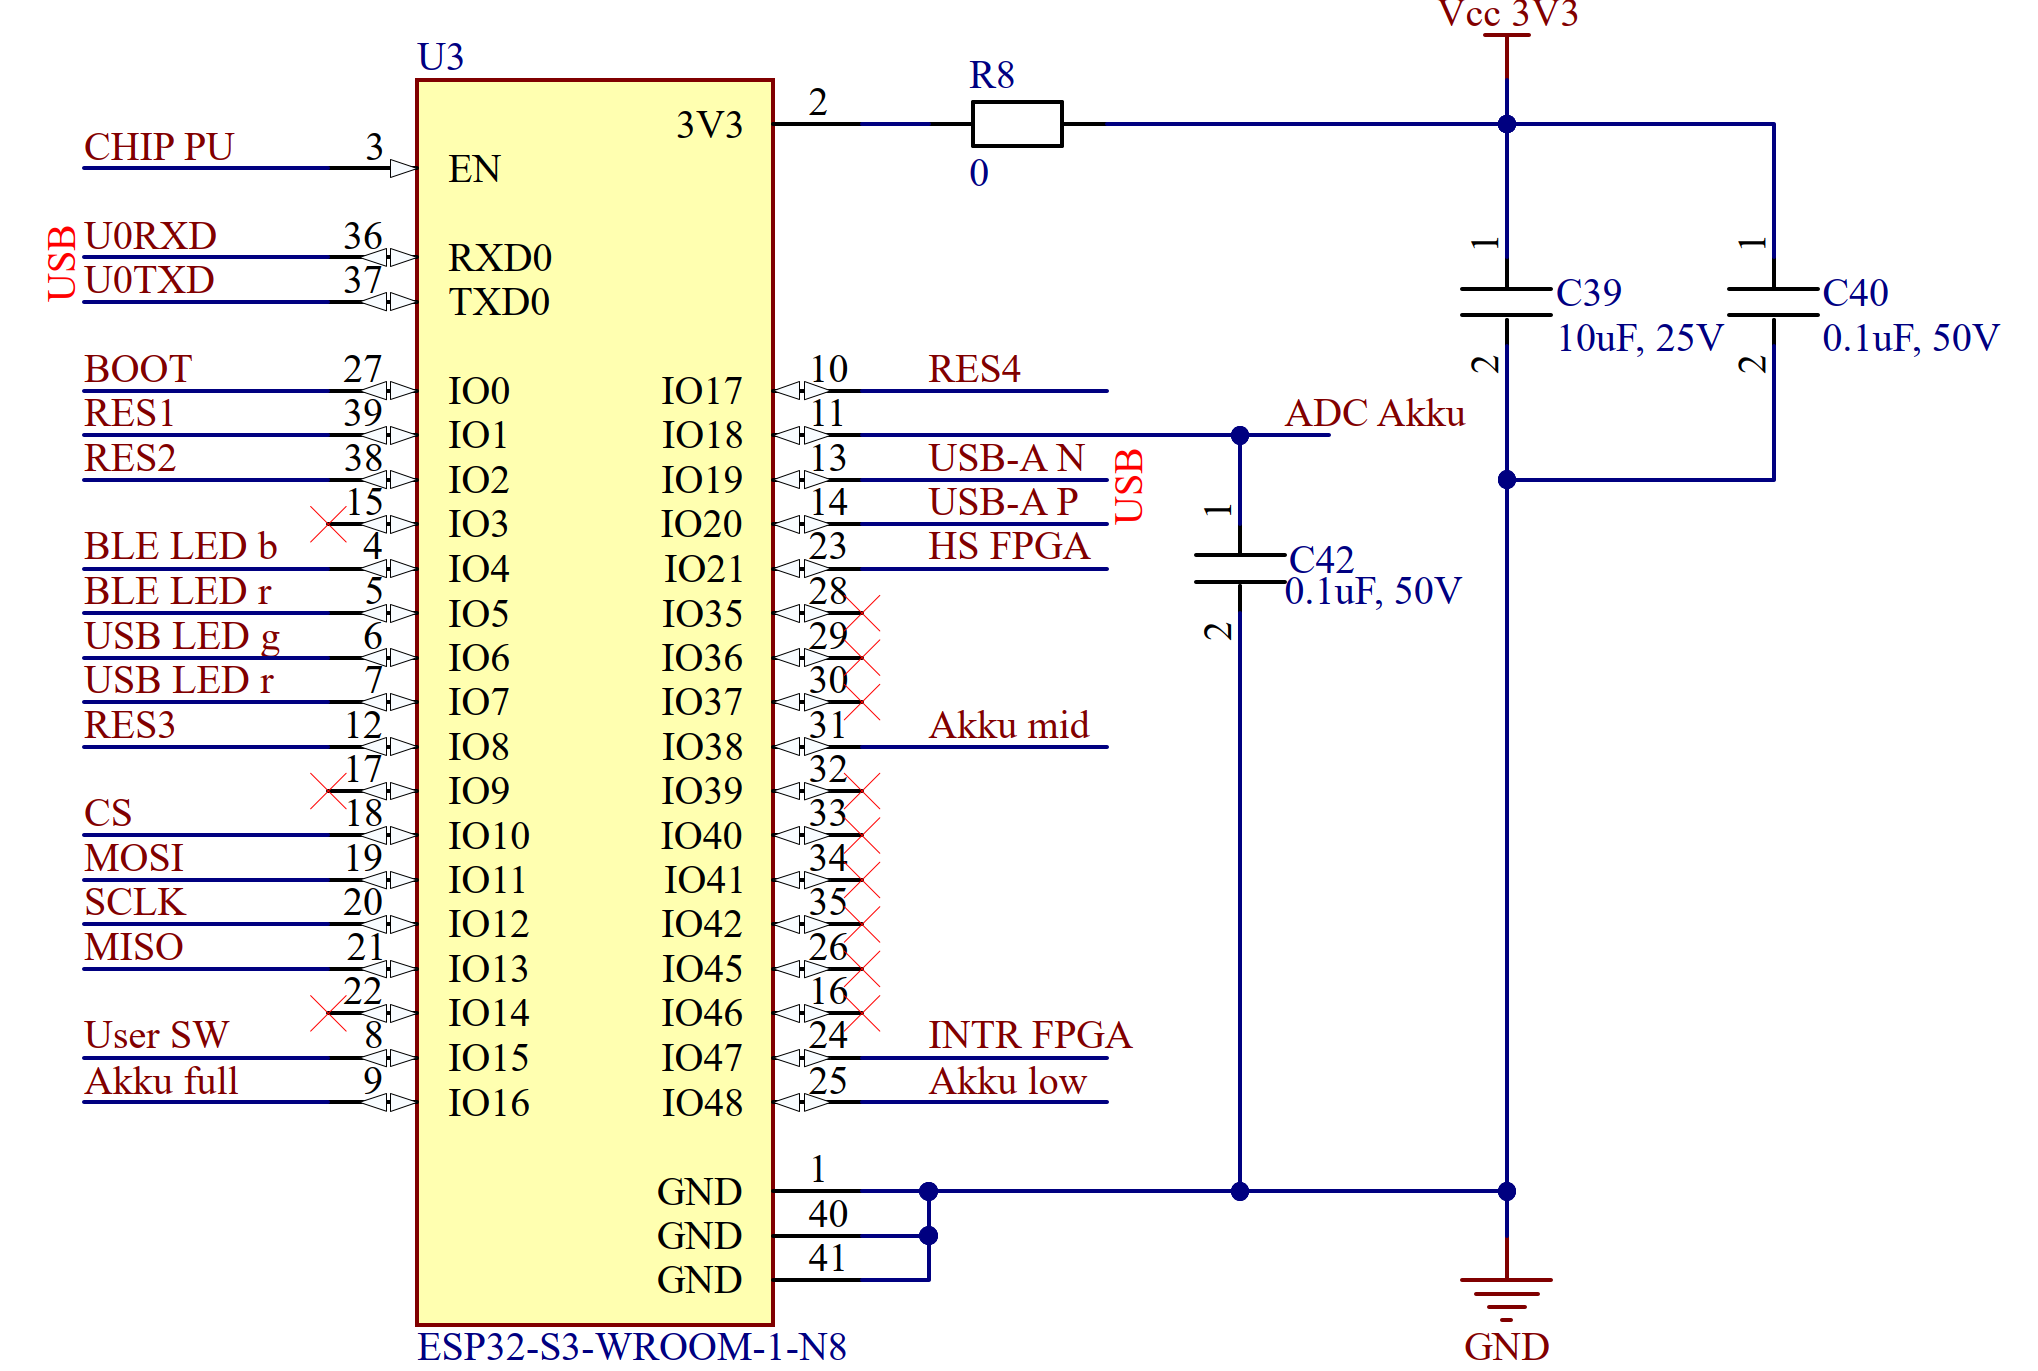
\includegraphics[width=0.8\linewidth]{Figures/Chap3/Schematics/ESP32.png}
    \caption{ESP32-S3}
    \label{fig:ESP32}
\end{figure}

Das Datenblatt sowie das Schema des ESP32-S3 Evaluationsboards befinden sich im Anhang \ref{app:File55} (Datenblatt) und \ref{app:File56} (Schema).

\subsection{Indikatoren}
\label{subsec:Indikatoren}
Zur Anzeige der Betriebszustände der Kommunikationsschnittstellen werden LEDs eingesetzt, die über den Darlington-Array-Transistor ULN2803CDWR vom ESP32-S3 oder FPGA angesteuert werden. Der ULN2803CDWR ermöglicht die Steuerung der LEDs, indem er acht Darlington-Transistorpaare integriert, die eine Stromverstärkung ermöglichen. Im Betrieb wird der Eingang eines Kanals auf HIGH geschaltet, wodurch der zugehörige Ausgang auf GND gezogen wird. Dadurch kann ein Laststrom durch die angeschlossene LED fliessen, welche mit einem Vorwiderstand betrieben wird, um den Strom zu begrenzen. Der Einsatz des ULN2803CDWR ermöglicht somit eine effiziente Steuerung der Statusanzeigen durch die digitalen Ausgänge des ESP32-S3 oder FPGA, ohne die Steuerlogik mit hohen Strömen zu belasten. Die Bluetooth-Schnittstelle wird durch eine blaue und eine rote LED signalisiert, während die USB-Schnittstellen mit einer grünen und einer roten LED dargestellt werden. Eine gelbe LED soll die Aktivität auf dem MVB anzeigen,  sobald der Sniffer angeschlossen wird. Zukünftig ist ein Akkubetrieb vorgesehen, weshalb auch eine Ladezustandsanzeige mittels LEDs eingeplant wurde. 
Das Datenblatt des ULN2803CDWR befindet sich im Anhang \ref{app:File57}.
\begin{figure}
    \centering
    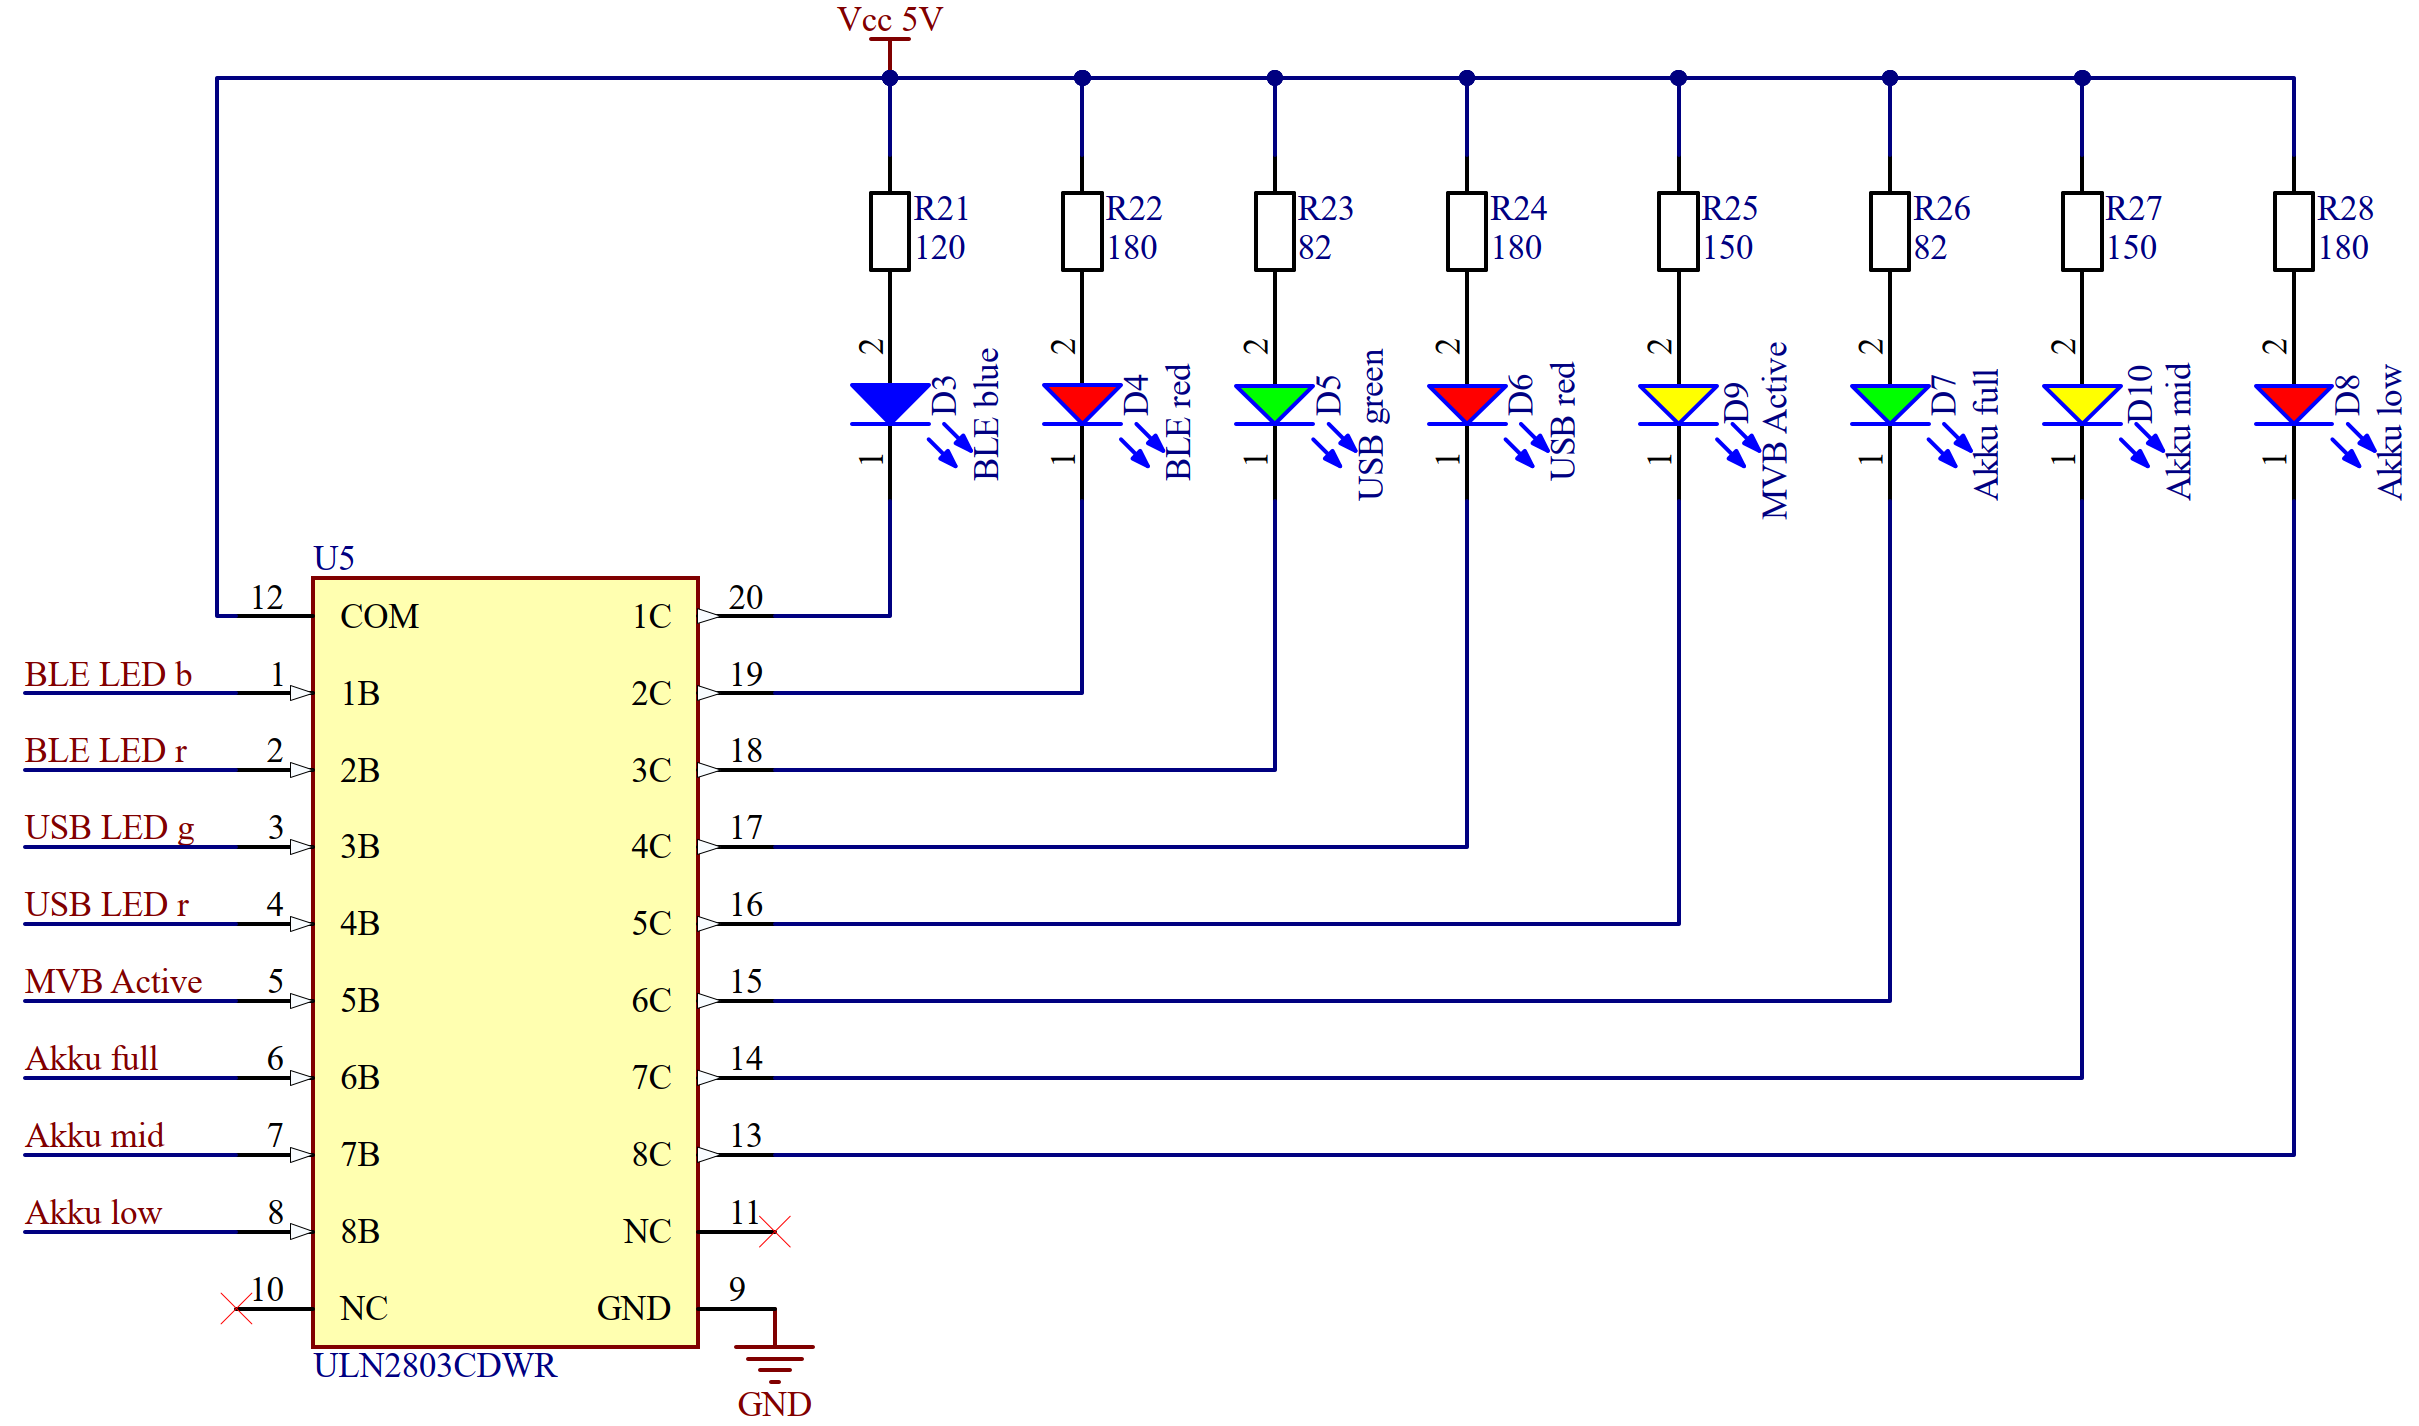
\includegraphics[width=0.9\linewidth]{Figures/Chap3/Schematics/Indicator_LEDs.png}
    \caption{Status LED}
    \label{fig:StateLED}
\end{figure}

\section{Testszenarien} %
In diesem Abschnitt werden die Testszenarien beschrieben, wie die einzelnen Hardwarekomponenten ESP32 und FPGA und die Verbindungstest zwischen den Komponenten gestestet wurde.

\subsection{ESP32 SPI und Statemachine Test}
\label{sub:ESPSPIundFSMTest}

Für die Verifikation der Firmware auf dem ESP32-S3 wurde ein zweites Gerät, welches als SPI-Master den FPGA simulieren soll, verwendet. Die Hardware, welche als SPI Master verwendet wurde war ein ESP32. Dies aus dem Grund, weil bereits Erfahrungen mit dem ESP32 vorhanden waren und ein Aufsetzten des Gerätes und Ausgeben schnell erreicht wurde. In Abbildung \ref{fig:TestszenarioESP32} ist der schematische Aufbau zu sehen. Es wurden die Verbindungen für die SPI-Leitungen und GND verbunden. Auf einem Laptop wurde die Open-Source-Software Bluetility verwendet, ein Bluetooth-Low-Energy-Tool. Mit dieser Anwendung können Geräte gescannt, deren Dienste und Eigenschaften durchsucht sowie Werte gelesen, geschrieben und abonniert werden. Gemäss Kapitel \ref{sub:BluetoothGATT} wurden die Daten in der Charakteristik mit der roten Zahl 1 empfangen. Zusätzlich wird die Reaktionszeit beim Empfangen der SPI-Daten gemessen. Dies wird durch das Vergleichen der Chip Select-Leitung und der Handshakeleitung. 

\begin{figure}[H]
    \centering
    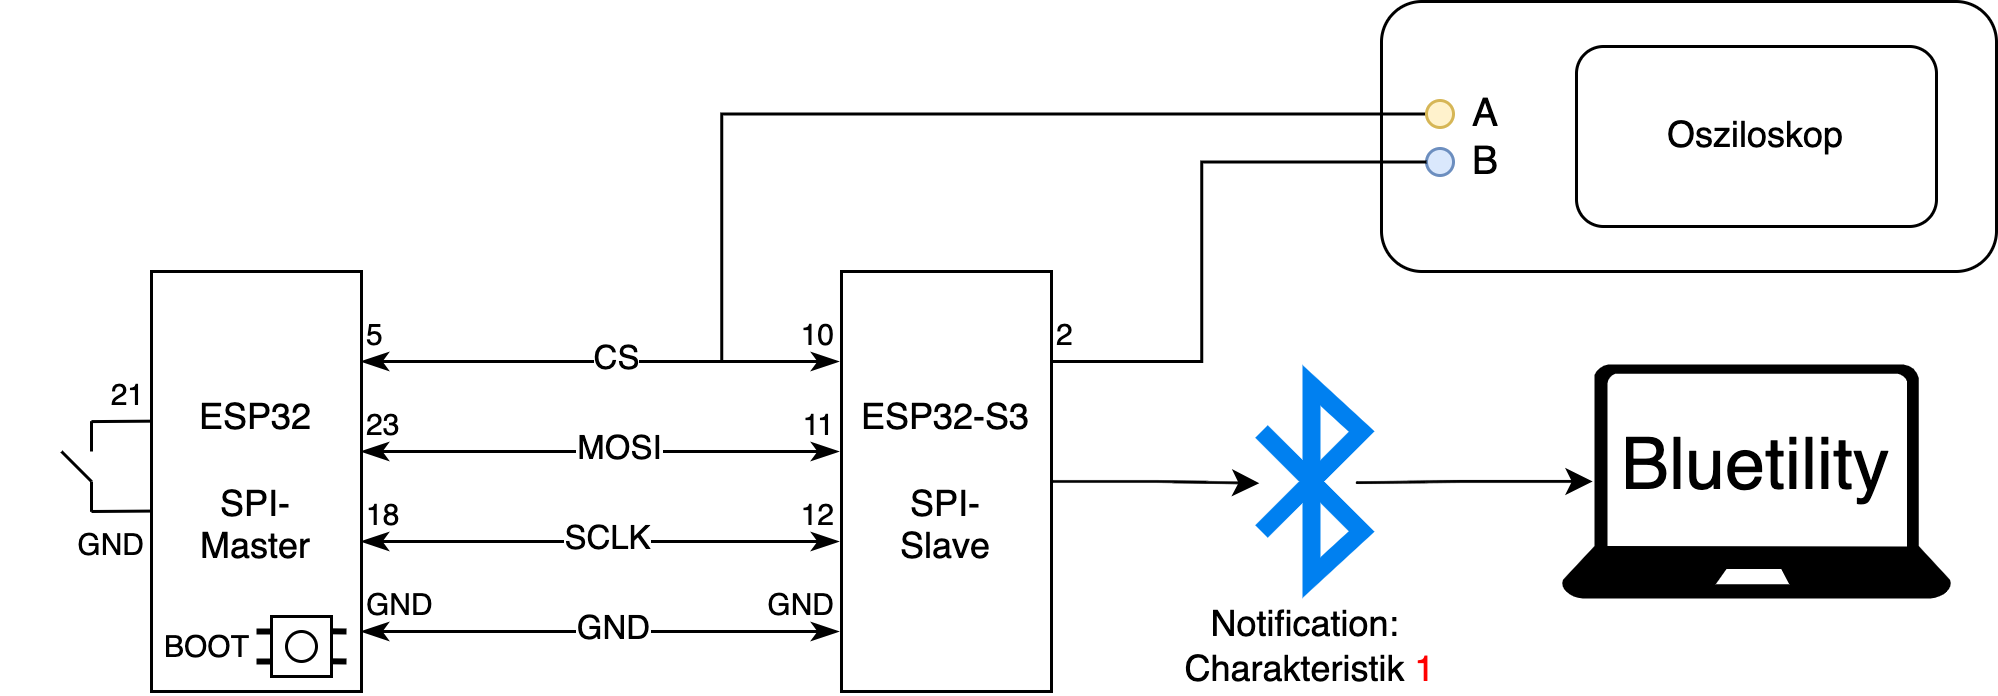
\includegraphics[width=0.9\linewidth]{Figures/Chap3/Testszenarien/Testszenario_ESP32.png}
    \caption{Testaufbau zum Testen der Manchester Decodierung auf dem ESP32-S3}
    \label{fig:TestszenarioESP32}
\end{figure}

Der SPI-Master konnte zwei unterschiedliche Telegramme schicken. Es kann entweder das kürzeste oder das längste Telegramm geschickt werden. Die Auswahl ist von Pin 21 (siehe Abbildung \ref{fig:TestszenarioESP32}) abhängig. Wird dieser Pin zu Ground gezogen, wird das lange Telegramm geschickt und wird der Kontakt offen gelassen, das Kurze. Das Senden eines Paketes wird durch Drücken des Boot-Knopfes ausgelöst. Dies zieht den Pin 0 zu Ground und das kann im Programm ausgewertet werden. 

Der Inhalt, der in Tabelle \ref{tab:TestDataESP32} zu sehen ist, sind die Nutzdatenbits, welche bei Bluetility ankommen sollen. Der SPI-Master schickt die Daten wie der FPGA Machnester Encodiert in 64 Bit-Päckchen, also jeweils 32 Bit Nutzdatenbits. Bei den Slave Daten wurde absichtlich ein lesbarer ASCII String für die Dummy Daten verwendet, da diese in Bluetility gleich ersichtlich ist.

\begin{table}[H]
    \centering
    \begin{tabular}{r||l|l}
         & Kurz & Lang\\ \hline
        FCode & 9 (0x9) & 12 (0xC)\\ \hline
        Addresse & 0x101 & 0x0D8\\ \hline
        Master Check & 0xF0 & 0x21\\ \hline
        Slave Data & NH & Hello World 01234567890123456789\\ \hline
        Slave Check & 0x53 & 0x5A 0x98 0x70 0x5d\\ 
    \end{tabular}
    \caption{Test Daten für Testszenario ESP32}
    \label{tab:TestDataESP32}
\end{table}




\subsection{Verbindungstest ESP32 zu FPGA}
\textcolor{red}{Wie wurde der Aufbau getestet}

Um zu testen ob die Decodierung des Manchestersignal bis hin zur Übertragung via Bluetooth korrekt funktioniert, wurde ein Testaufbau realisiert. Für den Aufbau wurden die verschiedenen Komponenten des Sniffers wie in Abbildung \ref{fig:AufbauSniffer} zu sehen ist, verbunden. Als Signalquelle wurde ein \textcolor{red}{\textit{Tektronix}} verwendet. Mit dem Tektronix ist es möglich über die beiden Outputs A \& B ein differentielles Signal auszugeben. Somit wurde das Signal welches zur Bestimmung der Busauslastung (siehe Kapitel \ref{fig:MessaufbauBusauslastungMessen}) aufgenommen wurde, mittels Matlab und \textcolor{red}{\textit{???Programm???}} so aufbereitet, dass dieses mit dem Tektronix abgespielt werden konnte.
Somit kann genau festgestellt werden ob die übertragenen Daten, dem Signal entsprechen und ob die Daten stabil und Fehlerfrei übertragen werden. Das Signal wurde zur Überprüfung im Vorhinein manuell decodiert.
Zur Prüfung wurden folgende Master und Slave Telegramme übertragen:

\begin{itemize}
  \item \textbf{Master Frame 1:}\hspace{0.5cm}0xC715'569A'6555'99A6\newline\textbf{Slave Frame 1:}\hspace{0.75cm}0xA8E3'5565'9A65'AAAA'AAAA'6A66
  \item \textbf{Master Frame 2:}\hspace{0.5cm}0xC715'5699'5A55'6AAA\newline\textbf{Slave Frame 2:}\hspace{0.75cm}0xA8E3'5565'A996'AAAA'AAAA'A569
  \item \textbf{Master Frame 3:}\hspace{0.5cm}0xC715'9656'5655'6AA9
\end{itemize}

Diese Telegramme entsprechen dem in \textit{Abbildung \ref{fig:AusschnittMvbOhneDds}} zu sehende Signal.

Die oben gezeigte Datenabfolge gibt Schlussendlich per Bluetooth folgenden Payload aus:

\begin{itemize}
  \item \textbf{Master Frame 1:}\hspace{0.5cm}0x1B'40'AD\hspace{1.5cm}\textbf{Slave Frame 1:}\hspace{0.5cm}0x04'B4'FF'FF'75
  \item \textbf{Master Frame 2:}\hspace{0.5cm}0x08'60'EF\hspace{1.7cm}\textbf{Slave Frame 2:}\hspace{0.5cm}0x00'00'FF
  \item \textbf{Master Frame 3:}\hspace{0.5cm}0x91'10'7E
\end{itemize}

%% !TEX root = ../main.tex

% Indicate the main file. Must go at the beginning of the file.

%---------------------------------------------------------------------
% CHAPTER TEMPLATE
%---------------------------------------------------------------------


\chapter{Methode} % Main chapter title
\label{ChapterX} % Change X to a consecutive number; for referencing this chapter elsewhere, use \ref{ChapterX}

%---------------------------------------------------------------------
% SECTION Busauslastung messen
%---------------------------------------------------------------------

\section{Busauslastung messen}
\textcolor{red}{Ein kurze Zusammenfasung, wie anhand einer Messug auf dem Bus mit Matlab ein Buslauslastung gemessen und ausgewertet wurde. Outcome präsentieren}

Um zu beurteilen, ob Bluetooth Low Energy (BLE) eine geeignete Lösung für die Übertragung von Telegrammen vom Sniffer zum Endgerät darstellt, wurde ein Versuch unternommen, die Busauslastung mittels Oszilloskop zu analysieren. Ziel war es, abzuschätzen, ob die dabei gewonnenen effektiven Nutzdaten über BLE übertragen werden können. Gleichzeitig sollte geprüft werden, ob eine direkte Übertragung aller Rohdaten möglich ist oder ob eine Filterung der Telegramme erforderlich wäre.

Für die Analyse wurden zwei Messungen durchgeführt: eine unter Normallast und eine unter Volllast. Die Volllast wurde simuliert, indem der Depot-Diagnosespeicher auf dem Fahrzeugdisplay angezeigt wurde. Dies führte dazu, dass der Speicher die entsprechenden Daten über den Bus an das Display sendete, was kurzfristig zu einer höheren Auslastung führte.

Die Messungen wurden mit einem Picoscope 2207B durchgeführt, während die anschließende Auswertung mit MATLAB realisiert wurde.

\subsection{Messaufbau}

Der Messaufbau ist in Abbildung \ref{fig:MessaufbauBusauslastungMessen} dargestellt. Um die Busauslastung zu messen, wurde die MVB-Leitung, die normalerweise von Gerät zu Gerät durchgeschleift ist, an einer geeigneten Stelle unterbrochen und ein Leitungsaufteiler eingefügt. Dies ermöglichte den direkten Zugriff auf die differentiellen Leitungen des Busses mit dem Picoscope. Der MVB-Loop wurde dabei wieder geschlossen, sodass keine Geräte vom Bus abgetrennt wurden. Die gemessenen Daten wurden über eine USB-Schnittstelle an einen Laptop übertragen und dort mit der Pico-Software aufgezeichnet.

\begin{figure}[H]
    \centering
    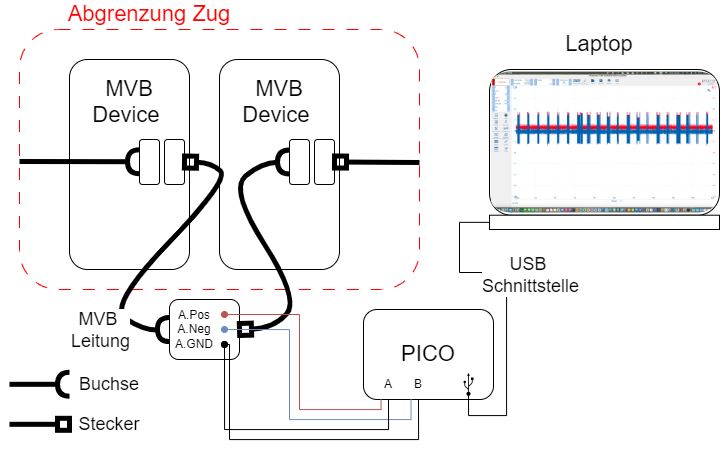
\includegraphics[width=0.8\linewidth]{Figures/Chap3/Busauslastung/Messaufbau_PICO_IC2000.png}
    \caption{Messaufbau Busauslastung messen}
    \label{fig:MessaufbauBusauslastungMessen}
\end{figure}

Die erfassten Daten wurden anschließend in das MATLAB-Dateiformat (.mat) exportiert. Die Struktur der MATLAB-Datei ist in Abbildung \ref{fig:MatlabFileStruktur} dargestellt. Die Variablen \textit{A} und \textit{B} entsprechen den Messpunkten des Picoscope, während \textit{Tinterval} die Zeit zwischen zwei Messpunkten angibt. 

\begin{figure}[H]
    \centering
    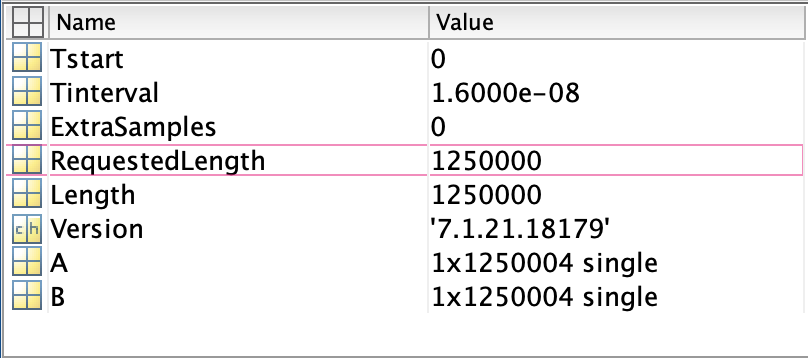
\includegraphics[width=0.5\linewidth]{Figures/Chap3/Busauslastung/Matlab_file_struktur.png}
    \caption{Matlab File Struktur}
    \label{fig:MatlabFileStruktur}
\end{figure}

Der Messaufbau blieb für die Messungen unter Normallast und Volllast identisch. Um die Volllast zu simulieren, wurde der Befehl zur Anzeige der Depot-Diagnosedaten auf dem Fahrzeugdisplay ausgelöst, bevor die Messung gestartet wurde. Der Zeitraum zwischen der Eingabe des Befehls und der Darstellung der Daten auf dem Display beträgt etwa 5 Sekunden.

\subsection{Matlab Auswertung}

\subsubsection{Variablen initialisieren}

\subsubsection{Delimiter erkennen}

\subsubsection{Nulldurchgänge}

\subsubsection{Auswertung Effektive Nutzdaten}







%----------------------------------------------------------------------
% SECTION Wahl der Hardware
%----------------------------------------------------------------------

\section{Design eigener Sniffer}
\textcolor{red}{Wie wurde der Sniffer aufgebaut. Schematischer Verlauf von D-Sub9 bis Endgerät soll aufgezeigt und erklärt werden.}

Für den ersten Entwurf des Sniffers wurde eine Anforderungsliste erstellt, in welcher die Fest- wie auch Wunschanforderungen definiert sind. In einem ersten Entwurf wurde schematisch dargestellt in welcher Reifenfolge welche Aufgabe won welcher Hardware durchgeführt werden soll. 

Dieser schematische Entwurf (siehe Abbildung x) zeigt die verschiedene Hardware auf und wie diese verbunden sind. Dabei wurden direkt die technischen Anforderungen, welche durch den MVB vorgegeben sind, im Schema dargestellt.

Um auf dem Differentiellen Signal ein einziges zu machen welches

Anhand dem ersten Entwurf, wurde eine graphische Darstellung aufgestellt (siehe Abbildung x) um die benötigten Komponente und den Datenfluss genauer darstellen zu können. Der MVB-Sniffer wurde in drei verschiedene Aufgabengebiete aufgeteilt. 
 

%----------------------------------------------------------------------
% SECTION Hadrware FPGA

%Themen nach Signalfluss aufbauen
%----------------------------------------------------------------------

\section{Hardware FPGA}
\textcolor{red}{Wie wurde das zu erreichende Ziel auf dem FPGA umgesetzt.}



\subsection{SPI}
\textcolor{red}{Wie wurde SPI implementiert. Welcher Mode, Geschindigkeit, Prinzip?}

\subsection{Manchester decodierung}
\textcolor{red}{Was ist die Überlegung hinter der decodierung des Manchester}


%----------------------------------------------------------------------
% SECTION Hardware PCB
%----------------------------------------------------------------------

\section{Hardware PCB}
\textcolor{red}{Wie wurde das zu erreichende Ziel auf dem PCB umgesetzt.}

\subsection{Design ESP32}
\textcolor{red}{Wie wurde der ESP auf der Platine integriert}

\subsection{Design FPGA}
\textcolor{red}{Wie wurde der FPGA auf der Platine integriert}



%----------------------------------------------------------------------
% SECTION Firmware ESP32
%----------------------------------------------------------------------

\section{Firmware ESP32}
\textcolor{red}{Wie wurde die Firmware auf dem ESP32 umgesetzt}

\subsection{Finite State Machine}
\textcolor{red}{Wie wurde das FreeRTOS benutzt, um die Zeitkritische Aufgaben zu lösen. Werlche Tasks und wele FSM arbeiten in den jeweiligen Cores}


\subsection{Bluetooth GATT-Server}
\textcolor{red}{Wie wurde der Bluetooth Gatt-Server aufgebaut. Erklärung Charakteristiken}





% !TEX root = ../main.tex

% Indicate the main file. Must go at the beginning of the file.

%--------------------------------------------------------------------------------
% CHAPTER Results
%--------------------------------------------------------------------------------


\chapter{Prototyp Sniffer} % Protoypen Test Main chapter title -> Sniffer Prototyp!?
\label{Prototyp Sniffer} % Change X to a consecutive number; for referencing this chapter elsewhere, use \ref{ChapterX}

%---------------------------------------------------------------------------------
% SECTION 1
%---------------------------------------------------------------------------------

\section{FPGA}
\label{sec:ResultatFPGA}
Der Test zur Datenauswertung im FPGA wurde, wie in Kapitel
\ref{sub:FPGADecSPITest} beschrieben, durchgeführt. Mittels der Software "'Picoscope 7"' konnten die ausgegebenen Daten \textit{MOSI} mit dem dazugehörigen \textit{SCLK} und dem Chipselect \textit{CS} gleich als SPI interpretiert und entschlüsselt dargestellt werden.
Im Verlaufe der Arbeit wurde das FPGA und dessen Decodierung in zwei Szenarien getestet.
Das eine Szenario ist der Test ohne die Zusatzimplementierung eines Puffers und somit das direkte Schreiben auf die SPI sobald ein Nutzdatenbyte ausgewertet wurde.
Im zweiten Szenario wurde ein 64 Bit grosser Puffer vor der SPI implementiert, um die Zeit zwischen der Datenübertragung auf der SPI zu verlängern.
In den folgenden Unterkapiteln werden die Resultate beider Szenarien aufgezeigt.

\subsection{Test ohne 64-Bit-Puffer Implementierung}
\label{sub:ResultatFPGAnoBuff}
Bei diesem Testszenario war kein Unterschied, ob das Signal alle 1 ms oder alle 100 ms übertragen wurde, feststellbar. In beiden Fällen werden mit
der Software \textit{Picoscope 7} die gleichen Übertragungsdaten angezeigt und somit die gleichen Werte entschlüsselt dargestellt.

In Abbildung \ref{fig:ResultatFPGANoBuff} ist dass vom Picoscope eingelesene SPI Signal mit MOSI, SCLK und CS zu sehen. Bei dieser Übertragung handelt es sich um ein Master-Frame.


\begin{figure}[H]
    \centering
    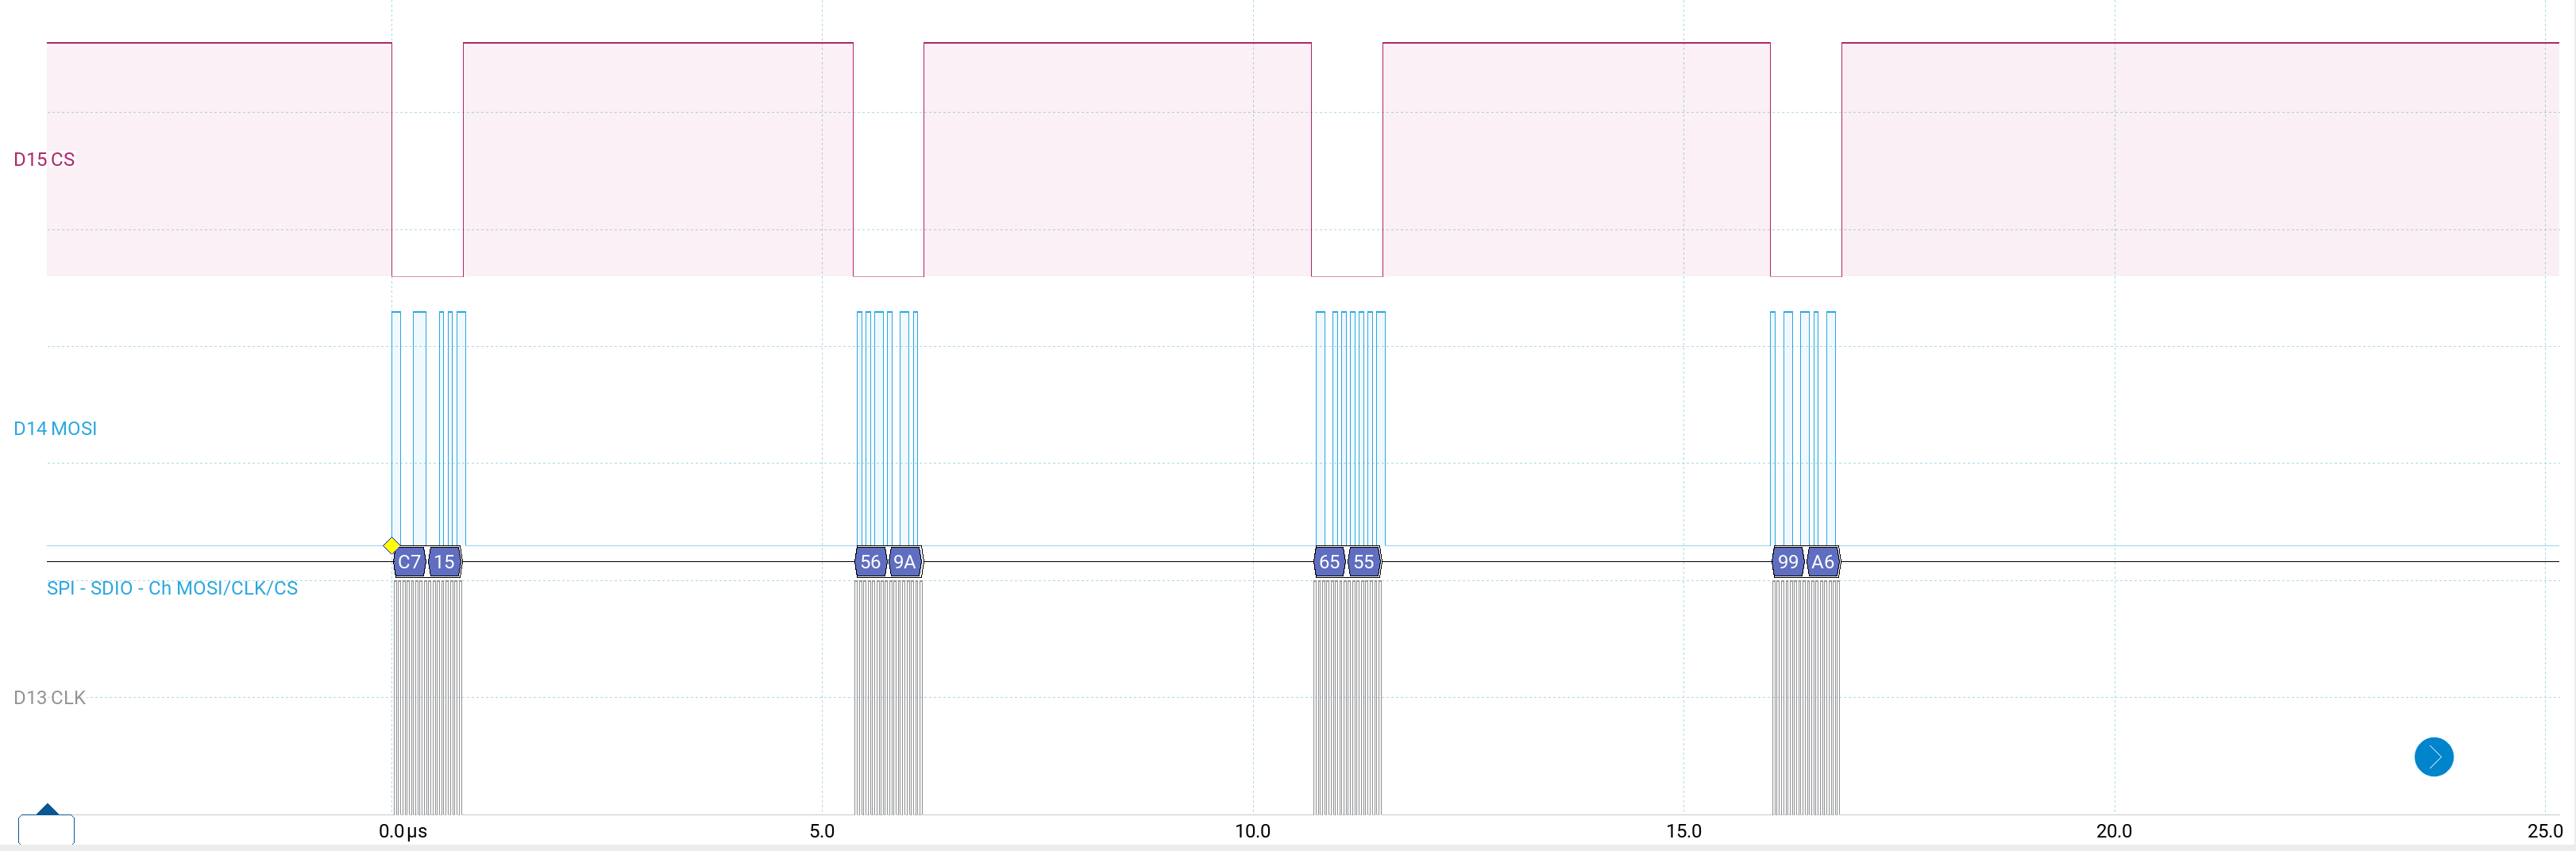
\includegraphics[width=1\linewidth]{Figures/Chap4/FPGA/Test_FPGA_noBuff_signal.png}
    \caption{Ausgegebene Daten des FPGA auf die SPI in Szenario 1 Nutzdatenbyte (16 Bit)}
    \label{fig:ResultatFPGANoBuff}
\end{figure}

Abbildung \ref{fig:ResultatFPGANoBuff} zeigt nur den ersten Teil der ganzen Übertragung. Das ganze übertragene Telegramm ist in Abbildung \ref{fig:ResultatFPGANoBuffFull} zu sehen. Aufgrund der Länge können die Daten nicht angezeigt werden, ohne hinein zu zoomen.
Es sind 32 Übertragungen an 16 Bit zu sehen, was 32 Nutzdatenbytes entsprechen. In der Tabelle \ref{tab:packet_data} sind die aus \textit{Picoscope 7} exportierten Daten aufgelistet, welche zur Abbildung \ref{fig:ResultatFPGANoBuffFull} gehören.

\begin{figure}[H]
    \centering
    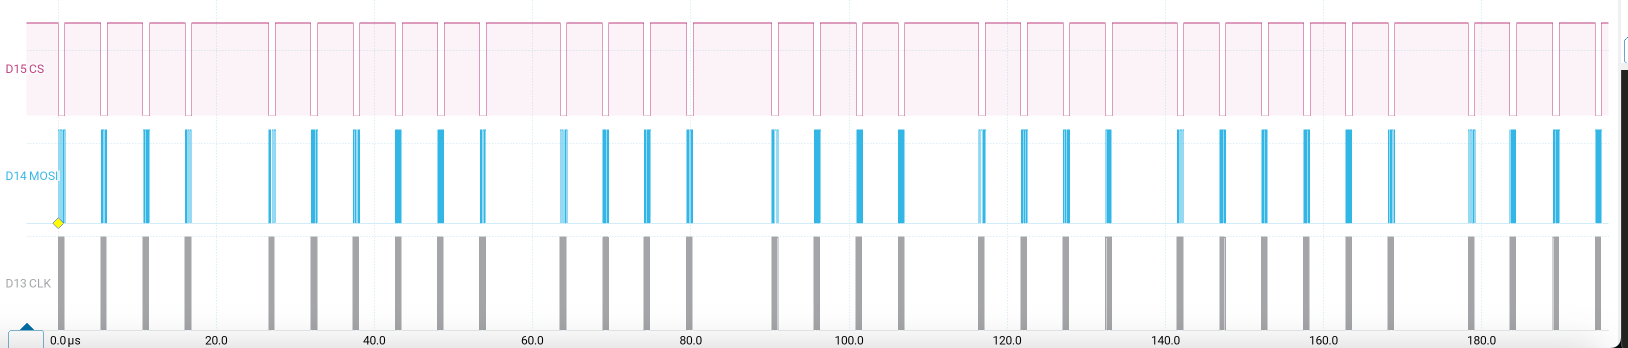
\includegraphics[width=1\linewidth]{Figures/Chap4/FPGA/Test_FPGA_noBuff_signal_full.png}
    \caption{Ausgegebenes ganzes Telegramm des FPGA auf die SPI in Szenario 1 Nutzdatenbyte (16 Bit)}
    \label{fig:ResultatFPGANoBuffFull}
\end{figure}

\begin{table}[h!]
    \centering
    \begin{tabular}{cl||cl||cl||cl}
        \toprule
        \textbf{Packet} & \textbf{Data} & \textbf{Packet} & \textbf{Data} & \textbf{Packet} & \textbf{Data} & \textbf{Packet} & \textbf{Data} \\ 
        \midrule
        1  & C7 15 & 9  & AA AA & 17 & 55 55 & 25 & A9 96 \\
        2  & 56 9A & 10 & 6A 66 & 18 & AA AA & 26 & AA AA \\
        3  & 65 55 & 11 & C7 15 & 19 & C7 15 & 27 & AA AA \\
        4  & 99 A6 & 12 & 55 95 & 20 & 56 99 & 28 & A5 69 \\
        5  & A8 E3 & 13 & 69 55 & 21 & 5A 55 & 29 & C7 15 \\
        6  & 55 65 & 14 & A9 AA & 22 & 6A AA & 30 & 96 56 \\
        7  & 9A 65 & 15 & A8 E3 & 23 & A8 E3 & 31 & 56 55 \\
        8  & AA AA & 16 & 55 55 & 24 & 55 65 & 32 & 6A A9 \\
        \bottomrule
    \end{tabular}
    \caption{Daten 16-Bit Übertragung}
    \label{tab:packet_data}
\end{table}

Die Abbildungen und die Tabelle entsprechen einem übertragenen Telegramm. Im Test fanden viel mehr Übertragungen statt. Dabei konnten keine, zu den gezeigten Daten, abweichenden Werte festgestellt werden.

\subsection{Test mit 64-Bit-Puffer Implementierung}
\label{sub:ResultatFPGABuff}
Im zweiten Testszenario konnten je nach Zeit, zwischen den gesendeten Telegramme, verschiedene Resultate beobachtet werden. In Abbildung \ref{fig:ResultatFPGABuff} ist die Übertragung eines ganzen Telegrammes zu sehen. In diesem Fall handelt es sich um die gleiche Anzahl übertragener Bit wie in Kapitel \ref{sub:ResultatFPGAnoBuff}, jedoch wurden diese jeweils in acht 64-Bit Pakete übertragen.

\begin{figure}[H]
    \centering
    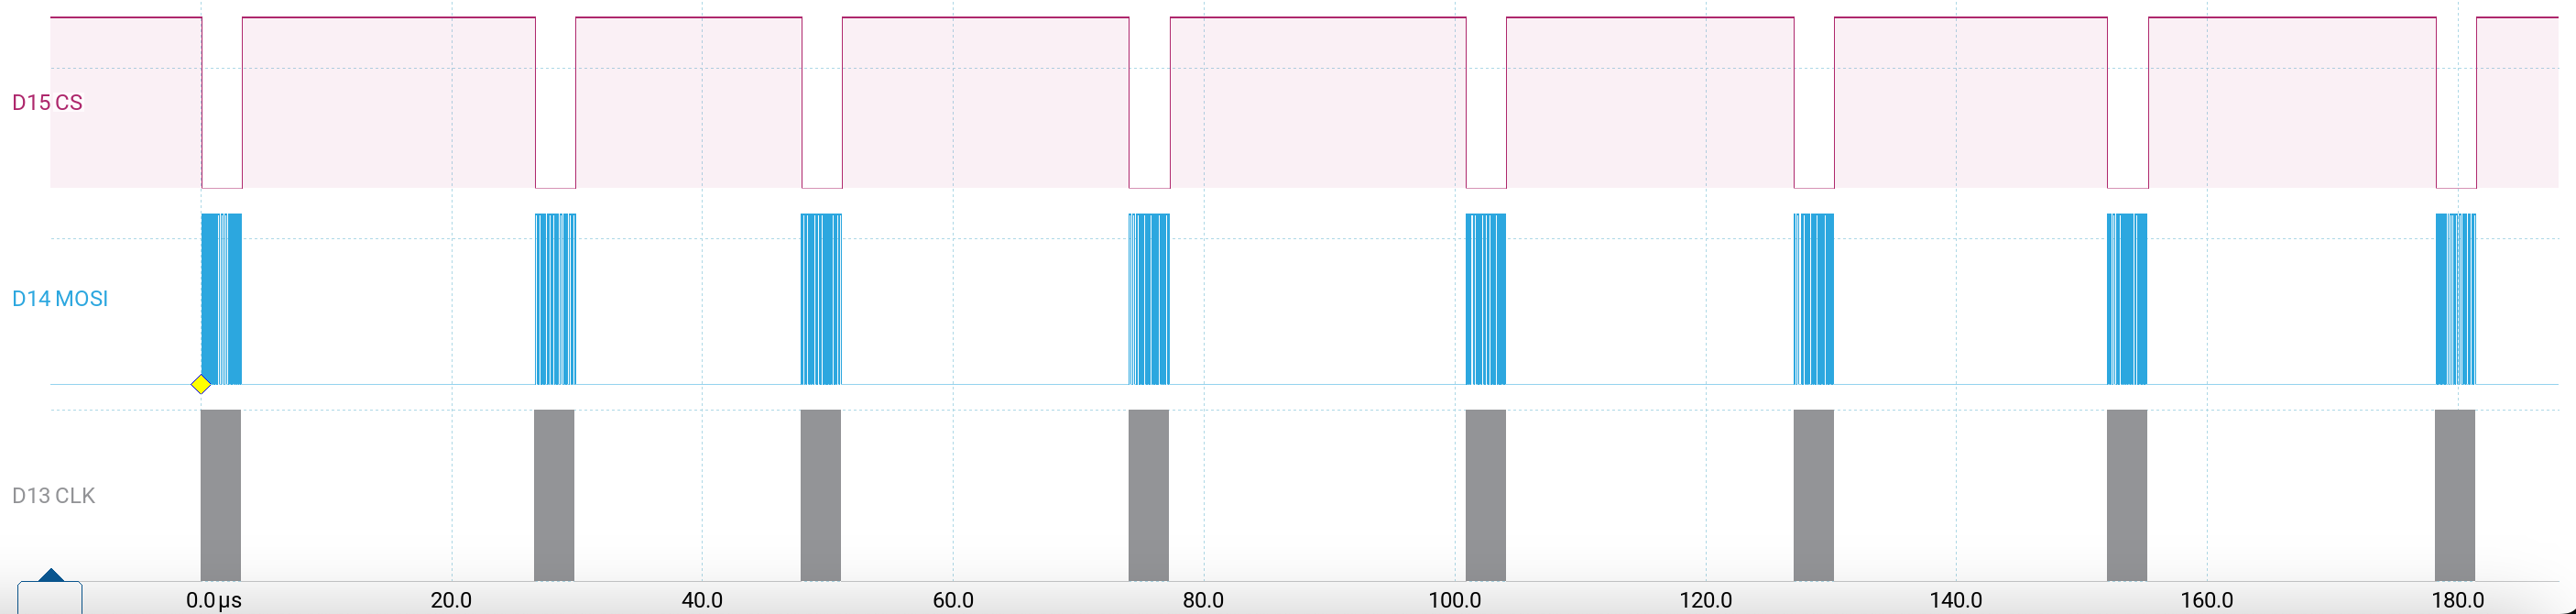
\includegraphics[width=1\linewidth]{Figures/Chap4/FPGA/Test_FPGA_Buff_signal.png}
    \caption{Ausgegebene Daten des FPGA auf die SPI in Szenario Puffer (64 Bit)}
    \label{fig:ResultatFPGABuff}
\end{figure}

Die übertragenen Daten, wenn alle 100 ms ein Telegramm ausgegeben wurde, sind in der Tabelle \ref{tab:packet_data_2cols} zu sehen. 

\begin{table}[h!]
    \centering
    \begin{tabular}{c||l}
        \toprule
        \textbf{Packet} & \textbf{Data} \\ 
        \midrule
        1 & C7 15 56 9A 65 55 99 A6 \\
        2 & A8 E3 55 65 9A 65 AA AA \\
        3 & AA AA 6A 66 C7 15 55 95 \\
        4 & 69 55 A9 AA A8 E3 55 55 \\
        5 & 55 55 AA AA C7 15 56 99 \\
        6 & 5A 55 6A AA A8 E3 55 65 \\
        7 & A9 96 AA AA AA AA A5 69 \\
        8 & C7 15 96 56 56 55 6A A9 \\
        \bottomrule
    \end{tabular}
    \caption{Übertragene Daten auf SPI; 100 ms; 64 Bit}
    \label{tab:packet_data_2cols}
\end{table}

Es ist zu sehen dass zwischen den erhaltenen Daten und den erwarteten Daten, welche in der Tabelle \ref{tab:frame_data} in der Spalte \textit{Data} abgebildet sind, keine Abweichungen festzustellen sind.

Wenn jede ms eine Übertragung statt findet, so sind zu den in der Tabelle \ref{tab:frame_data} sehende Anordnung der Daten, Abweichungen festzustellen. Grundsätzlich werden die gleichen Daten übermittelt aber oftmals an einer anderen Stelle und teilweise wurden nicht alle Pakete übertragen. Selten werden auch falsche Daten übermittelt.

In der Tabelle \ref{tab:data_table} sind die Daten eines Telegramms zu sehen, welches fehlerhaft war. Beim Achten Packet ist zu sehen dass anstatt \textit{"'C7 15 96 56 56 55 6A A9"'} die falschen Daten \textit{"'00 0F 8E 2B 2C AC AC AA"'} übermittelt wurden.

\begin{table}[h!]
    \centering
    \begin{tabular}{c||l}
        \toprule
        \textbf{Packet} & \textbf{Data} \\ 
        \midrule
        1 & C7 15 56 9A 65 55 99 A6 \\
        2 & A8 E3 55 65 9A 65 AA AA \\
        3 & AA AA 6A 66 C7 15 55 95 \\
        4 & 69 55 A9 AA A8 E3 55 55 \\
        5 & 55 55 AA AA C7 15 56 99 \\
        6 & 5A 55 6A AA A8 E3 55 65 \\
        7 & A9 96 AA AA AA AA A5 69 \\
        8 & 00 0F 8E 2B 2C AC AC AA \\
        \bottomrule
    \end{tabular}
    \caption{Übertragene Daten auf SPI; 1 ms; 64 Bit}
    \label{tab:data_table}
\end{table}




%---------------------------------------------------------------------------------
% SECTION 2
%---------------------------------------------------------------------------------

\section{Firmware ESP32}
\label{sec:ResultatESP32}
%\textcolor{red}{Erstes Resultat des ESP: SPI ist nicht genügend schnell, um die Packete des FPGA entgegen zu nehmen}

Der Test der Firmware des ESP32-S3 wurde gemäss Kapitel \ref{sub:ESPSPIundFSMTest} durchgeführt. Als Erstes wurde das kurze Telegramm getestet und der Pin 21 wurde nicht auf Ground verbunden. Durch Drücken der Boot-Taste auf dem SPI-Master wird das Senden getriggert. In Abbildung \ref{fig:ResultatBLEKurz} ist die Anzeige in der Applikation \textit{Bluetility} gezeigt und Einfärbungen gemacht, welche Teile zu den Daten gehören.

\begin{figure}[H]
    \centering
    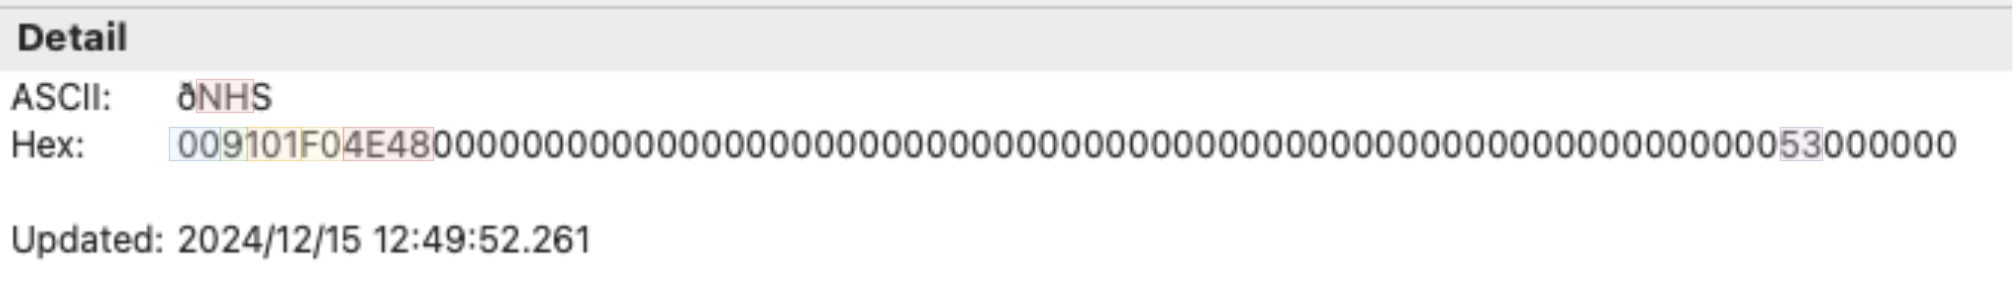
\includegraphics[width=0.9\linewidth]{Figures/Chap4/ESP32/Resultat_BLE_kurz.png}
    \caption{Resultat Bluetility kurzes Telegram}
    \label{fig:ResultatBLEKurz}
\end{figure}

Die Daten werden in der Struktur aus Kapitel \ref{subsub:DataTelegramm} übertragen und sind wie folgt:

\begin{itemize}[noitemsep]
    \item metadata: 0x00 --> Keine Fehler im Telegramm
    \item data\_m: 0x9101 --> FCode: 9; Adresse: 0x101
    \item check\_m: 0xF0 --> Dummy Check Data
    \item data\_s: 0x4E48 --> ASCII für "'NH"'
    \item check\_s: 0x53 --> Dummy Check Data
\end{itemize}

%Die Aufzeichnung der Reaktionszeit für das kurze Telegramm mit dem Oszilloskop ist in Abbildung \ref{fig:ReakKurz} zu sehen. Die orange Linie ist dabei die \textit{Chip Select} Leitung und die blaue Linie die \textit{Handshakeleitung}. 

\begin{figure}[H]
    \centering
    % Erstes Bild
    \begin{subfigure}[b]{0.45\textwidth}
        \centering
        \includegraphics[width=\linewidth]{Figures/Chap4/ESP32/Gesammte Transaktion Kurz.JPG} 
        \caption{Insgesamt 2 Transaktionen}
        \label{fig:GesTransKurz}
    \end{subfigure}
    \hfill 
    %Zweites Bild
    \begin{subfigure}[b]{0.45\textwidth}
        \centering
        \includegraphics[width=\linewidth]{Figures/Chap4/ESP32/Reaktionszeit Kurz.JPG} 
        \caption{Vergrösserung im Zeitbereich der Reaktionszeit bei kurzem Telegramm}
        \label{fig:ReakKurz}
    \end{subfigure}
    \caption{Resultat der Reaktionszeit kurzes Telegramm gemessen mit dem Oszilloskop}
    \label{fig:ResultatOsziReaktionKurz} 
\end{figure}

In Abbildung \ref{fig:GesTransKurz} ist ersichtlich, dass das vollständige Telegramm nach 2 Transaktionen abgeschlossen ist. Dies kann anhand der negativen Pulse der Chip-Select Leitung gezählt werden.
In Abbildung \ref{fig:ReakKurz} sind die Zeiten gut zu sehen. Die in Kapitel \ref{sub:ESPSPIundFSMTest} definierten Zeiten lauten:
\begin{itemize}
    \item Reaktionszeit: 2 $\mu$s
    \item BTR-Zeit: 12 $\mu$s
\end{itemize}


Als Zweites wurde das lange Telegramm getestet. In Abbildung \ref{fig:ResultatBLELang} ist die Anzeige in der Applikation \textit{Bluetility} gezeigt und Einfärbungen gemacht, welche Teile zu den Daten gehören.

\begin{figure}[H]
    \centering
    \includegraphics[width=0.9\linewidth]{Figures/Chap4/ESP32/Resultat_BLE_lang.png}
    \caption{Resultat Bluetility langes Telegram}
    \label{fig:ResultatBLELang}
\end{figure}

Die Daten werden wieder in der Struktur aus Kapitel \ref{subsub:DataTelegramm} übertragen und sind wie folgt:

\begin{itemize}[noitemsep]
    \item metadata: 0x00 --> Keine Fehler im Telegramm
    \item data\_m: 0xC0B8 --> FCode: 0xC (12); Adresse: 0x0B8
    \item check\_m: 0x21 --> Dummy Check Data
    \item data\_s: \textit{siehe Bild} --> ASCII für "'Hello World 01234567890123456789"'
    \item check\_s: 0x5A'98'70'5D --> Dummy Check Data der Reihe nach 0x[0]'[1]'[2]'[3]
\end{itemize}

\begin{figure}[H]
    \centering
    % Erstes Bild
    \begin{subfigure}[b]{0.45\textwidth}
        \centering
        \includegraphics[width=\linewidth]{Figures/Chap4/ESP32/Gesammte Transaktion Lang.JPG} 
        \caption{Insgesamt 11 Transaktionen}
        \label{fig:GesTransLang}
    \end{subfigure}
    \hfill 
    %Zweites Bild
    \begin{subfigure}[b]{0.45\textwidth}
        \centering
        \includegraphics[width=\linewidth]{Figures/Chap4/ESP32/Reaktionszeit Lang.JPG} 
        \caption{Vergrösserung im Zeitbereich der Reaktionszeit bei langem Telegramm}
        \label{fig:ReakLang}
    \end{subfigure}
    \caption{Resultat der Reaktionszeit langem Telegramm gemessen mit dem Oszilloskop}
    \label{fig:ResultatOsziReaktionLang} 
\end{figure}

In Abbildung \ref{fig:GesTransLang} ist ersichtlich, dass das vollständige Telegramm nach 11 Transaktionen abgeschlossen ist. Dies kann anhand der negativen Pulse der Chip-Select Leitung gezählt werden.
In Abbildung \ref{fig:ReakLang} sind die Zeiten zu sehen. Die in Kapitel \ref{sub:ESPSPIundFSMTest} definierten Zeiten lauten:
\begin{itemize}
    \item Reaktionszeit: 2 $\mu$s
    \item BTR-Zeit: 12 $\mu$s
\end{itemize}


%\href{https://docs.espressif.com/projects/esp-idf/en/stable/esp32s3/api-reference/peripherals/spi_slave.html#transaction-interval}{ESP-IDF SPI Slave Transaction Interval}


\section{Übertragungstest SPI}
\label{sec:ResultatÜbertragungSPI}
Um die Übertragung der Daten vom FPGA zum ESP32-S3 zu überprüfen, wurde ein Test gemäss Kapitel \ref{subsec:VerbindugstestESP32FPGA} durchgeführt.

Für das Triggerintervall von 3 Sekunden ist folgendes Resultat entstanden. Auf der \textit{Bluetify}-Applikation sind die folgenden Notifikationen empfangen worden:

\begin{table}[H]
    \centering
    \begin{tabular}{r||c|c|c|c}
        \hline
        Frame Nr & 1 & 2 & 3 & 4\\ \hline
        meta data & 0x00 & 0x00 & 0x00 & 0x01\\ \hline
        data\_m & 0x1B40 & 0x0860 & 0x1A30 & 0x9110\\ \hline
        check\_m & 0xAD & 0xEF & 0x7F & 0x7E\\ \hline
        data\_s & 0x04B4FFFF & 0x0000 & 0x04E9FFFF & -\\ \hline
        check\_s & 0x75 & 0xFF & 0xC6 & -\\ \hline
    \end{tabular}
    \caption{Empfangene Telegramme bei Triggerinterval 3 s}
    \label{tab:EmpfTeleg3sTrigg}
\end{table}

Mit dem Picoscope wurde das Signal im digitalen Bereich aufgezeignet, sodass die Reaktionszeit und die Back-to-Receive-Zeit bestimmt werden konnten. 

\begin{figure}
    \centering
    \includegraphics[width=\linewidth]{Figures/Chap4/Verbindungstest_SPI/VerbindungstestZeiten.png}
    \caption{Erstes 64-Bit Packet}
    \label{fig:VerbindungstestZeiten}
\end{figure}

In Abbildung \ref{fig:VerbindungstestZeiten} ist die Messung mit dem Picoscope zu sehen. Die oberste Kurve ist die Clock-Leitung, darunter folgt die MOSI-Leitung, darunter in Blau dargestellt die Chip-Select-Leitung und zu unterst die Handshake-Leitung.

Die in Kapitel \ref{sub:ESPSPIundFSMTest} definierten Zeiten lauten:
\begin{itemize}
    \item Reaktionszeit: 2 $\mu$s
    \item BTR-Zeit: 12 $\mu$s
\end{itemize}


\section{Stresstest FPGA und ESP32}
\label{sec:ResStresstest}

Der Stresstest wurde, wie in Kapitel \ref{sub:MethStesstest} beschrieben, durchgeführt.

Das Resultat für das Triggerintervall von 50 ms ist in Abbildung \ref{fig:Stress50} zu sehen. Die gemessenen Telegramme für die Erstellung der Grafik ist in Anhang \ref{app:File63_50ms} zu finden. Die vier häufigsten Telegramme sind die erwarteten Telegramme aus Tabelle \ref{tab:frame_data}.

\begin{figure}[H]
    \centering
    \begin{minipage}{0.29 \textwidth}
        \begin{tabular}{c||c}
            \toprule
            \textbf{Anzahl} & \textbf{Frame Nr} \\ 
            \midrule
            469 &  1\\
            469 & 2 \\
            469 & 3 \\
            468 & 4 \\
            \bottomrule
        \end{tabular}
    \end{minipage}
    \hfill
    \begin{minipage}{0.7 \textwidth}
        \includegraphics[width = \linewidth]{Figures/Chap4/Stesstest/Stress_50.png}
    \caption{Stresstest Triggerintervall 50 ms}
    \label{fig:Stress50}
    \end{minipage}
\end{figure}


Das Resultat für das Triggerintervall von 25 ms ist in Abbildung \ref{fig:Stress25} zu sehen. Die gemessenen Telegramme für die Erstellung der Grafik ist in Anhang \ref{app:File64_25ms} zu finden. Die vier häufigsten Telegramme sind die erwarteten Telegramme aus Tabelle \ref{tab:frame_data}.

\begin{figure}[H]
    \centering
    \begin{minipage}{0.29 \textwidth}
        \begin{tabular}{c||c}
            \toprule
            \textbf{Anzahl} & \textbf{Frame Nr} \\ 
            \midrule
            932 & 1\\
            932 & 2\\
            929 & 3\\
            925 & 4\\
            \bottomrule
        \end{tabular}
    \end{minipage}
    \hfill
    \begin{minipage}{0.7 \textwidth}
        \includegraphics[width=\linewidth]{Figures/Chap4/Stesstest/Stress_25.png}
    \caption{Stresstest Triggerintervall 25 ms}
    \label{fig:Stress25}
    \end{minipage}
\end{figure}

Das Resultat für das Triggerintervall von 12.5 ms ist in Abbildung \ref{fig:Stress12_5} zu sehen. Die gemessenen Telegramme für die Erstellung der Grafik ist in Anhang \ref{app:File65_12_5ms} zu finden. Die vier häufigsten Telegramme sind die erwarteten Telegramme aus Tabelle \ref{tab:frame_data}.

\begin{figure}[H]
    \centering
    \begin{minipage}{0.29 \textwidth}
        \begin{tabular}{c||c}
            \toprule
            \textbf{Anzahl} & \textbf{Frame Nr} \\ 
            \midrule
            1600 & 1\\
            1553 & 2\\
            1468 & 4\\
            1340 & 3\\
            \bottomrule
        \end{tabular}
    \end{minipage}
    \hfill
    \begin{minipage}{0.7 \textwidth}
        \includegraphics[width=\linewidth]{Figures/Chap4/Stesstest/Stress_12_5.png}
    \caption{Stresstest Triggerintervall 12.5 ms}
    \label{fig:Stress12_5}
    \end{minipage}
\end{figure}

\newpage

Das Resultat für das Triggerintervall von 1 ms ist in Abbildung \ref{fig:Stress1} zu sehen. Die gemessenen Telegramme für die Erstellung der Grafik ist in Anhang \ref{app:File66_1ms} zu finden. Die vier häufigsten Telegramme sind die erwarteten Telegramme aus Tabelle \ref{tab:frame_data}.

\begin{figure}[H]
    \centering
    \begin{minipage}{0.29 \textwidth}
        \begin{tabular}{c||c}
            \toprule
            \textbf{Anzahl} & \textbf{Frame Nr} \\ 
            \midrule
            6191 & 4\\
            891 & 2 \\
            720 & 1 \\
            507 & 3 \\
            \bottomrule
        \end{tabular}
    \end{minipage}
    \hfill
    \begin{minipage}{0.7 \textwidth}
        \includegraphics[width=\linewidth]{Figures/Chap4/Stesstest/Stress_1.png}
    \caption{Stresstest Triggerintervall 1 ms}
    \label{fig:Stress1}
    \end{minipage}
\end{figure}

Zusammenfassend wurden vier Messungen von ungefähr 20-30 Sekunden durchgeführt und die resultierenden Plots eingefügt.

\section{Hardware Design}
\label{sec:ResultatHardware}
Im Rahmen dieser Arbeit wurde ein Schema für den MVB-Sniffer in der Software Altium entworfen. Es wurde darauf geachtet, die zentralen Rollen der Komponenten, übersichtlich zu gestalten, dass ihre Interaktionen und Funktionalitäten nachvollziehbar sind. Diese wurden ebenfalls detailliert im Kapitel \ref{sec:Hardware Design} erläutert. Das entwickelte Schema erfüllt die aktuellen Anforderungen von den zusammengeführten Evaluationsboards, wurde kompakter gestaltet durch Reduzierung von nicht benötigter Komponenten und Verbindungen und bietet eine Basis für zukünftige Erweiterungen des Sniffers. 

Das Schema ist auf 5 Seiten aufgeteilt. Auf der ersten Seite befinden sich die Anschlüsse an den MVB, die Verbindung zu dem RS485-Transreceiver und alle In- und Outputs von den Banken. Die zweite Seite wurde für die DC/DC-Wandler verwendet, die Interaktionen die über Taster und einen Schalter mit dem FPGA gemach twerden können, sowie die JTAG Schnittstelle und der Oszillator für den FPGA. Auf der dritten Seite sind die Spannungsversorgungen und Ground Anbindungen. Seite 4 zeigt den ESP32, dessen USB Schnittstellen, den 3 Drucktastern für Interaktionen mit dem ESP32, die USB-UART-Brücke und die Transistoren Schaltung um den ESP32 in die 3 Modi zu versetzen. Auf der Seite 5 ist der Darlington-Array für die Ansteuerung der Zustands LED und die Pinleiste, sowie der Spannungsteiler für die zukünftige Akkumessung. 

Der gesamte Altium Projektordner befindet sich gezippt im Anhang \ref{app:File58}.







% \section{Resultat} % 
% \textcolor{red}{Was ist beim Test herausgekommen. Was hat funktionniert, was nicht?}


% !TEX root = ../main.tex

% Indicate the main file. Must go at the beginning of the file.

%--------------------------------------------------------------------------------
% CHAPTER TEMPLATE
%--------------------------------------------------------------------------------


\chapter{Diskussion} % Main chapter title
\label{chapter5:Diskussion} % Change X to a consecutive number; for referencing this chapter elsewhere, use \ref{ChapterX}

%--------------------------------------------------------------------------------
% SECTION "Erreichte Ziele"
%--------------------------------------------------------------------------------

% \section{Erreichte Ziele}
% \label{sec:ErreichteZiele}
% \textcolor{red}{Welche Ziele wurden erreicht. Welche Ziele wurden nicht erreicht und wieso}


% \section{MVB Sniffer}
% \label{sec:DiskussionSniffer}

% \subsection{SPI Übertragung}
% \label{sec:DiskussionSPI}

% \subsection{subs2}
% \label{sec:}

% \subsection{subs3}
% \label{sec:}

In diesem Kapitel wird der Prototyp "'MVB-Sniffer"' den definierten Zielen gegenübergestellt und diskutiert. Erhaltene Resultate bei den verschiedenen Testszenarien, wie diese in Kapitel \ref{sec:Testszenarien} beschrieben wurden, werden mit den erwarteten Daten verglichen. Des Weiteren werden in der Projektarbeit festgestellte Herausforderungen näher erläutert und mögliche Lösungsansätze besprochen.

\section{Hardware FPGA}
\label{sec:DiskussionHardwareFPGA}
In diesem Kapitel werden die erhaltenen Resultate gemäss Kapitel \ref{sec:ResultatFPGA} mit den erwarteten Daten gemäss Kapitel \ref{sub:FPGADecSPITest} diskutiert.

Wurde das Telegramm alle 100 ms übertragen, so konnten die erwarteten Daten korrekt empfangen werden. Wurde das generierte Signal aber jede ms gesendet, so gelang die Übertragung, nur im Falle ohne die Implementierung des 64-Bit Puffers, wie erwartet.

Das Abtasten des Manchestersignal und die ununterbrochene Übertragung eines Nutzdatenbytes über SPI funktioniert fehlerfrei und sehr stabil.
Dies zeigt auf, dass die Decodierungslogik des FPGA wie auch die Ausgabe auf die SPI korrekt und robust funktioniert.

Sobald das ausgewertete Signal, und somit der Bitstream über den 64-Bit Puffer geleitet wird, entstehen teilweise Fehler in der Übertragung.
Diese Fehler zeigen sich indem in einzelnen Fälle Daten in der Übertragung fehlen, oder auch falsche Daten übermittelt werden.
Es kann keine Regelmässigkeit festgestellt werden, um welche Daten es sich dabei handelt und in welchem Abstand diese Fehler auftreten.

Die genaue Ursache für die teilweise fehlenden oder falschen Daten in der Übertragung konnte nicht festgestellt werden.



\section{Firmware ESP32-S3}
\label{sec:DiskussionFirmwareESP32}
Die erwarteten Werte aus Kapitel \ref{sub:ESPSPIundFSMTest} konnten in den Resultaten bestätigt werden. Der SPI-Master konnte, ohne einen Softwaredelay innerhalb des Programms zu verwenden, maximal alle 40 $\mu$s ein Paket mit 64 Bit an Daten versenden. Dies entspricht nicht den genannten Anforderungen des FPGA, welches ein SPI-Paket mit 64 Bit an Daten alle 24 $\mu$s schickt. 

Der Test hat jedoch gezeigt, dass die Daten korrekt von der SPI-Schnittstelle empfangen werden, durch die spi\_queue richtig weitergegeben werden und von der State-Machine richtig verarbeitet werden. Der Pointer auf die aktuell abgespeicherten Daten wird korrekt über die ble\_queue weitergegeben und die Notification richtig verarbeitet und dem verbundenen Endgerät mitgeteilt. 

Die Abbildungen \ref{fig:ReakKurz} und \ref{fig:ReakLang} zeigen, dass die Reaktionszeit 2 $\mu$s beträgt, bis die SPI-Peripherie nach Abschluss der Transaktion reagiert. Dies ist ein grosser Wert, für das eigentlich die Geschwindigkeit eines Interrupts erwartet wurde, welcher beinahe instantan auslöst.

Diese Zeit lässt sich mit der Erklärung in der Slave Driver API Reference erklären. Die nachfolgende Erklärung wurde aus dem englischen Übersetzt: 

\textit{Die ESP32-S3 SPI-Slave Peripherie ist als "'general purpose Device"' entwickelt und wird von der CPU gesteuert. [...] Alle Transaktionen müssen von der CPU durchgeführt werden, was bedeutet, dass das Senden und Empfangen nicht Echtzeit stattfinden und vielleicht bemerkbare Latenz vorhanden sind.} \cite{SPI_SLAVE_DRIVER_API}

Dies schränkt die Nutzbarkeit der SPI-Peripherie ein. Die Transaktionslänge hängt zudem nicht mit dieser Zeit zusammen. Vergleichbare Zeiten wurden ebenfalls bei 16 oder 32 Bit an Daten gemessen. 

Die Back-to-Receive-Zeit (BTR-Zeit) entspricht einem akzeptablen Wert von 12 $\mu$s. Da jede 24 $\mu$s ein neues 64-Bit Paket empfangen wird, hat die SPI-Peripherie genug Zeit, um auch bei grösserer Auslastung zu funktionieren. Eine Verkürzung der Übertragungspakete auf 32-Bit ist nicht sinnvoll, da 32-Bit Pakete jede 12 $\mu$s empfangen werden müssten und das nicht gewährleistet werden kann. 

\section{Übertragung SPI}
\label{sec:DiskussionÜbertragungSPI}

Der Übertragungstest des SPI-Protokolls zwischen FPGA und ESP32-S3 war erfolgreich. Die Ergebnisse in Tabelle \ref{tab:EmpfTeleg3sTrigg} und Abbildung \ref{fig:VerbindungstestZeiten} bestätigen die Funktionalität der Kommunikation.

Die Metadaten des vierten Frames (0x01) zeigen korrekt an, dass das Telegramm nur mit einem Master-Frame gesendet wurde. Während einer 60-sekündigen Messung wurden alle Telegramme korrekt empfangen. Die gemessenen Zeiten für Reaktion 2 $\mu$s und Back-to-Receive 12 $\mu$s entsprechen den Anforderungen aus Kapitel \ref{sub:ESPSPIundFSMTest}.

Die Busauslastung war im Test nicht repräsentativ für reale Szenarien, weshalb zusätzliche Stresstests durchgeführt wurden (Kapitel \ref{sec:DiskStresstest}). Diese dienen der Validierung unter höherer Belastung.

Zusammenfassend arbeitet das System stabil und erfüllt die Anforderungen bei der Verarbeitung der Daten, vorbehaltlich der Ergebnisse des Stresstests.

\section{Stressteset SPI-Übertragung}
\label{sec:DiskStresstest}
Die Messungen wurden jeweils ungefähr 20-30 Sekunde durchgeführt. Der Stresstest hat gezeigt, dass die Belastungsgrenze zwischen 25 ms und 12.5 ms liegen muss. 

In Abbildung \ref{fig:Stress50} und Abbildung \ref{fig:Stress25} sind mehrheitlich vier verschiedene Telegramme zu sehen, welche empfangen werden. Die vier meist empfangenen Telegramme sind die erwarteten Telegramme.

Ab der Messung bei 12.5 ms (Abbildung \ref{fig:Stress12_5}) wird die Fehlerquote grösser. Viele Werte wurden nur 1 - 20 Mal empfangen, was darauf hindeutet, dass einzelne Fehler in den Telegrammen passiert sind. Die vier meist empfangenen Telegramme sind jedoch die erwarteten Telegramme.


Bei der Messung mit einem Triggerintervall von 1 ms (Abbildung \ref{fig:Stress1}) ist die Differenz noch grösser. Jedoch auch hier sind die vier meist empfangenen Telegramme die Erwarteten. Hier aber mit einer grösseren Differenz als sonst. Die Telegrammnummer 4 wurde vermutlich am meisten übertragen, weil dies lediglich eine SPI-Transaktion von 32 Nutzdatenbits benötigt, welche alle auf einmal übertragen werden. 

Was aus dieser Messung nicht gesehen werden kann, ist, an welcher Stelle die Fehler in den Telegrammen entstehen und dafür sind folgende Orte möglich:
\begin{itemize}[]
    \item Die Daten werden vom FPGA falsch über SPI versendet
    \item Die hohe Frequenz an SPI-Transaktionen kann vom ESP32-S3 nicht verarbeitet werden
    \item Die Daten werden Firmware intern nicht integer behandelt und Buffer werden überschrieben.
    \item Der ESP32-S3 schickt die Daten nicht korrekt.
    \item Das Python Script ist nicht leistungsfähig genug, die hohe Frequenz an Daten korrekt entgegenzunehmen
\end{itemize}

Zudem kann auch nicht genau gesagt werden, wie viele Trigger über den Zeitraum der Messung aufgetreten sind.

Aufgrund fehlender Zeit kann dies nicht mehr weiterverfolgt und gemessen werden. Da bereits beim FPGA Übertragungsprobleme bei höherer Busauslastung erkannt wurden (siehe Kapitel \ref{sec:DiskussionHardwareFPGA}) und die in der Firmware verwendeten Buffer nicht durch Semaphore oder Mutex geschützt sind, könnte auch eine Kombination aus den oben genannten Problemen zu dem Fehlerbild bei 1 ms Triggerintervall in Abbildung \ref{fig:Stress1} führen.


\section{Prototyp Sniffer}
\label{sec:DiskussionSniffer}
Das Minimal-Value Ziel wie es in der Tabelle \ref{tab:minvalueproduct} festgehalten ist, konnte nur teilweise erreicht werden. Die Auswertung und Übertragung bis hin zur Ausgabe per Bluetooth eines MVB-Telegramms funktioniert fehlerfrei. Jedoch wurde im FPGA kein Zeitstempel implementiert, und weiter konnte das PCB in Altium nicht fertiggestellt werden.

Hauptursachen zur Nichterreichung des Zieles sind aufgetretene Fehler in der Entwicklung und die fehlende Zeit zum Schluss der Projektarbeit. Dadurch, dass Quartus zur Entwicklung und Synthetisierung des VHDL-Codes sowie Altium zur Entwicklung des PCBs neue Entwicklungsumgebungen waren, in denen noch keine Kenntnisse vorhanden waren, wurde mehr Zeit als geplant aufgewendet, um die Umgebungen und deren Prozesse kennenzulernen, sodass ein erfolgreicher Sniffer entwickelt werden kann.


Zu Beginn der Projektarbeit wurde ein Zeitplan (siehe Anhang \ref{app:Zeitplan}) erstellt, in welchem die zu erledigenden Arbeiten mit deren Sollzeit aufgelistet sind. Es ist zu sehen, dass viele Abweichungen zwischen "'Ist"' und "'Soll"' festzustellen sind. Diese Abweichungen sind, wie bereits erwähnt, auf die Probleme in der Entwicklung und die längere Zeit zur Einarbeitung in die Entwicklungsumgebungen zurückzuführen. In der Mitte der Projektarbeit wurde ein Minimal-Value Ziel definiert. Daraufhin wurden einige geplante Aufgaben nicht mehr weiterverfolgt. Diese Aufgaben sind im Zeitplan unter "'Ist"' mit "'nicht ausgeführt"' vermerkt.

\chapter{Ausblick} % Main chapter title
\label{chapter6:Ausblick} % Change X to a consecutive number; for referencing this chapter elsewhere, use \ref{ChapterX}
% !TEX root = ../main.tex

% Indicate the main file. Must go at the beginning of the file.

%----------------------------------------------------------------------------------------
% CHAPTER TEMPLATE
%----------------------------------------------------------------------------------------


%\chapter{Verzeichnisse} % Main chapter title

%\label{ChapterX} % Change X to a consecutive number; for referencing this chapter elsewhere, use \ref{ChapterX}

%----------------------------------------------------------------------------------------
% SECTION 1
%----------------------------------------------------------------------------------------

% \section{Literaturverzeichnis}

%\section{Quellenverzeichnis}
\addcontentsline{toc}{chapter}{Literaturverzeichnis}
\printbibliography

%\newpage

%\section{Abbildungsverzeichnis}
\listoffigures
%\newpage


%\section{Tabellenverzeichnis}
\listoftables     % Add list of tables
%\newpage

%\section{Abkürzungsverzeichnis}
% % !TEX root = ../main.tex

%----------------------------------------------------------------------------------------
% ABBREVIATIONS
%----------------------------------------------------------------------------------------

% Liste der Abkürzungen: eine zweispaltige Tabelle.
\begin{abbreviations}{ll}

\textbf{LAH} & \textbf{L}ist \textbf{A}bbreviations \textbf{H}ere\\
\textbf{WSF} & \textbf{W}hat (it) \textbf{S}tands \textbf{F}or\\

\end{abbreviations}


%----------------------------------------------------------------------------------------
% PHYSICAL CONSTANTS/OTHER DEFINITIONS
%----------------------------------------------------------------------------------------

%% List of physical constants: a three column table
%\begin{constants}{lr@{${}={}$}l} 
%
%% The \SI{}{} command is provided by the siunitx package, see its documentation 
%% for instructions on how to use it
%
%Speed of Light & $c_{0}$ & \SI{2.99792458e8}{\meter\per\second} (exact)\\
%%Constant Name & $Symbol$ & $Constant Value$ with units\\
%
%\end{constants}


%----------------------------------------------------------------------------------------
% SYMBOLS
%----------------------------------------------------------------------------------------

%% List of Symbols: a three column table
%\begin{symbols}{lll} 
%
%$a$ & distance & \si{\meter} \\
%$P$ & power & \si{\watt} (\si{\joule\per\second}) \\
%%Symbol & Name & Unit \\
%
%\addlinespace % Gap to separate the Roman symbols from the Greek
%
%$\omega$ & angular frequency & \si{\radian} \\
%
%\end{symbols}

%\newpage



%-----------------------------------
% SUBSECTION 1
%-----------------------------------
%\subsection{Aufgabenstellung}


%-----------------------------------
% SUBSECTION 2
%-----------------------------------

%\subsection{Subsection 2}

%----------------------------------------------------------------------------------------
% SECTION 2
%----------------------------------------------------------------------------------------

%\section{Aufgabenstellung}



%----------------------------------------------------------------------------------------
% LIST OF ABBREVIATIONS / SYMBOLS / FIGURES/TABLES PAGES
%----------------------------------------------------------------------------------------

%% !TEX root = ../main.tex

%----------------------------------------------------------------------------------------
% ABBREVIATIONS
%----------------------------------------------------------------------------------------

% Liste der Abkürzungen: eine zweispaltige Tabelle.
\begin{abbreviations}{ll}

\textbf{LAH} & \textbf{L}ist \textbf{A}bbreviations \textbf{H}ere\\
\textbf{WSF} & \textbf{W}hat (it) \textbf{S}tands \textbf{F}or\\

\end{abbreviations}


%----------------------------------------------------------------------------------------
% PHYSICAL CONSTANTS/OTHER DEFINITIONS
%----------------------------------------------------------------------------------------

%% List of physical constants: a three column table
%\begin{constants}{lr@{${}={}$}l} 
%
%% The \SI{}{} command is provided by the siunitx package, see its documentation 
%% for instructions on how to use it
%
%Speed of Light & $c_{0}$ & \SI{2.99792458e8}{\meter\per\second} (exact)\\
%%Constant Name & $Symbol$ & $Constant Value$ with units\\
%
%\end{constants}


%----------------------------------------------------------------------------------------
% SYMBOLS
%----------------------------------------------------------------------------------------

%% List of Symbols: a three column table
%\begin{symbols}{lll} 
%
%$a$ & distance & \si{\meter} \\
%$P$ & power & \si{\watt} (\si{\joule\per\second}) \\
%%Symbol & Name & Unit \\
%
%\addlinespace % Gap to separate the Roman symbols from the Greek
%
%$\omega$ & angular frequency & \si{\radian} \\
%
%\end{symbols}

% \bibliography{example}
%\listoffigures    % Add list of figures
%\listoftables     % Add list of tables


%----------------------------------------------------------------------------------------
% THESIS CONTENT - APPENDICES
%----------------------------------------------------------------------------------------
\appendix % Cue to tell LaTeX that the following "chapters" are Appendices

%\renewcommand{\chaptermark}[1]{\markboth{Appendix \thechapter}{}}
% Include the appendices of the thesis as separate files from the Appendices folder
% Uncomment the lines as you write the Appendices
% !TEX root = ../main.tex

%----------------------------------------------------------------------------------------
% APPENDIX A
%----------------------------------------------------------------------------------------
\chapter{PDF Abgaben}
\label{AppendixA}

\textbf{A.1 Zeitplan\\
A.2 Aufgabenstellung\\
A.3 Verwendete Tools\\
A.4 Flankenerkennung Bits für Startdelimiter\\
A.5 Manchester Decoding State Machine\\
A.6 Schemata}


\includepdf[pages=1,pagecommand={\thispagestyle{headings} \section{Zeitplan} \label{app:Zeitplan}}, scale=0.9]{Appendices/Zeitplan.pdf}

\newpage

\includepdf[pages=1,pagecommand={\thispagestyle{headings} \section{Aufgabenstellung} \label{app:Aufgabenstellung}}, scale=0.8]{Appendices/PA_renn_Multifunction Vehicle Bus Sniffer_V1.pdf}


\includepdf[pages=2,pagecommand={\thispagestyle{headings}}, scale=0.8]{Appendices/PA_renn_Multifunction Vehicle Bus Sniffer_V1.pdf}



% For referencing this appendix elsewhere, use \ref{AppendixA}
%

%\section{How do I change the colors of links?}
%
%The color of links can be changed to your liking using:
%
%{\small\verb!\hypersetup{urlcolor=red}!}, or
%
%{\small\verb!\hypersetup{citecolor=green}!}, or
%
%{\small\verb!\hypersetup{allcolor=blue}!}.
%
%\noindent If you want to completely hide the links, you can use:
%
%{\small\verb!\hypersetup{allcolors=.}!}, or even better: 
%
%{\small\verb!\hypersetup{hidelinks}!}.
%
%\noindent If you want to have obvious links in the PDF but not the printed text, use:
%
%{\small\verb!\hypersetup{colorlinks=false}!}
%
%\section{How can I add a Figure in the Appendix?}
%
%You can refer to a figure in the Appendix (like \ref{fig:appendix-figure}) and it will show up as expected.
%
%\begin{figure}
%\includegraphics[width=0.25\textwidth]{../Figures/Bart_Simpson.png}
%\centering
%\caption[A random appendix figure]{Bart Simpson. (2023, May 17). In Wikipedia. \url{https://en.wikipedia.org/wiki/Bart_Simpson}}
%\label{fig:appendix-figure}
%\end{figure}


\newpage  % Fügt einen Seitenumbruch ein

\section{Verwendete Tools}
\label{app:VerwendeteTools}

% \begin{table}[H]
%     \centering
%     %\begarin{tabular}{p{2.5cm}p{2cm}p{8.5cm}}
%     \begin{tabular}{>{\raggedright\arraybackslash}p{3cm} >{\raggedright\arraybackslash}p{2cm} >{\raggedright\arraybackslash}p{8cm}}
%     \toprule
%         Programm & Version & Downloadlink\\
%     \midrule
%         ESP-IDF & v5.1.1 & https://github.com/espressif/\mbox{esp-idf}\allowbreak/tree/v5.1.1\\ \hline
%         Visual Studio Code & 1.96.0 & https://code.visualstudio.com/docs/\\  \hline
%         ESP-IDF \mbox{Extension for} VS Code & 1.9.0 & https://marketplace.visualstudio.com\allowbreak/items?itemName=espressif.esp-idf-extension\\  \hline
%         PicoScope 7 TM & 7.1.21.18179 & https://www.picoauto.com/downloads\\ \hline
%         Altium Designer & 24.9.1 (Build 31) & https://www.altium.com/de/products\allowbreak/downloads \\  \hline
%         Intel® Quartus® Prime Lite Edition Software & 23.1.1 & https://www.intel.com/content/www/us\allowbreak/en/software-kit/825278/intel-quartus-prime-lite-edition-design-software-version-23-1-1-for-windows.html\\ \hline
%         Matlab & R2023\_a & von Hochschule bereitgestellt \\ \hline
%         ArbExpress & 3.6 & von Betreuungsperson bereitgestellt \\ \hline
%         Python & 3.10.7 & https://www.python.org/downloads/ \\\hline
%         Bluetility & 1.5.1 & https://github.com/jnross/Bluetility \\
%     \bottomrule
%     \end{tabular}
%     \caption{Verwendete Software-Tools}
%     \label{tab:UsedTools}
% \end{table}


\begin{table}[H]
    \centering
    \begin{tabular}{>{\raggedright\arraybackslash}p{6cm} || >{\raggedright\arraybackslash}p{4cm} || >{\raggedright\arraybackslash}p{3cm}}
    \toprule
        Programm & Version & Downloadlink\\
    \midrule
        ESP-IDF & 5.1.1 & \href{https://github.com/espressif/esp-idf/tree/v5.1.1}{Link} \\ \hline
        Visual Studio Code & 1.96.0 & \href{https://code.visualstudio.com/docs/}{Link} \\ \hline
        ESP-IDF \mbox{Extension for} VS Code & 1.9.0 & \href{https://marketplace.visualstudio.com/items?itemName=espressif.esp-idf-extension}{Link} \\ \hline
        PicoScope 7 TM & 7.1.21.18179 & \href{https://www.picoauto.com/downloads}{Link} \\ \hline
        Altium Designer & 24.9.1 (Build 31) & \href{https://www.altium.com/de/products/downloads}{Link} \\ \hline
        Intel® Quartus® Prime Lite Edition Software & 23.1.1 & \href{https://www.intel.com/content/www/us/en/software-kit/825278/intel-quartus-prime-lite-edition-design-software-version-23-1-1-for-windows.html}{Link} \\ \hline
        Matlab & R2023\_a & von Hochschule bereitgestellt \\ \hline
        ArbExpress & 3.6 & von Betreuungsperson bereitgestellt \\ \hline
        Python & 3.10.7 & \href{https://www.python.org/downloads/}{Link} \\ \hline
        Bluetility & 1.5.1 & \href{https://github.com/jnross/Bluetility}{Link} \\ \hline
        Draw IO & 25.0.2 & \href{https://github.com/jgraph/drawio-desktop/releases/tag/v25.0.2}{Link} \\ \hline
        ChatGPT & Model 4 & \href{https://chatgpt.com}{Aufruflink}\\
    \bottomrule
    \end{tabular}
    \caption{Verwendete Software-Tools}
    \label{tab:UsedTools}
\end{table}

\newpage

\section{Flankenerkennung Bits für Startdelimiter}
\label{app:Flankenerkennung Bits}

\begin{figure}[H]
    \centering
    \includegraphics[width=\linewidth]{Figures/Chap3/Busauslastung/Master_Startdel.png}
    \caption{Anzahl Flanken in einem Master Startdelimiter ist 7}
    \label{fig:MasterStartdel}
\end{figure}

\begin{figure}[H]
    \centering
    \includegraphics[width=\linewidth]{Figures/Chap3/Busauslastung/Slave_Startdel.png}
    \caption{Anzahl Flanken in einem Slave Startdelimiter ist 7}
    \label{fig:SlaveStartdel}
\end{figure}

\newpage
\includepdf[pages=1,pagecommand={\thispagestyle{headings} \section{Manchester Decoding State Machine} \label{app:ManchDec}}, scale=0.9]{Appendices/State_Machine_Manchester.pdf}


\includepdf[pages=2,pagecommand={\thispagestyle{headings}}, scale=0.9]{Appendices/State_Machine_Manchester.pdf}


\newpage
\includepdf[pages=1, angle=90,pagecommand={\thispagestyle{headings} \section{Schemata} \label{app:Schemata}}, scale=0.75]{Appendices/SchematicsV1_2.pdf}
\label{app:Schema.pdf}

\includepdf[pages=2, angle=90,pagecommand={\thispagestyle{headings}}, scale=0.8]{Appendices/SchematicsV1_2.pdf}

\includepdf[pages=3, angle=90,pagecommand={\thispagestyle{headings}}, scale=0.8]{Appendices/SchematicsV1_2.pdf}

\includepdf[pages=4, angle=90,pagecommand={\thispagestyle{headings}}, scale=0.8]{Appendices/SchematicsV1_2.pdf}

\includepdf[pages=5, angle=90,pagecommand={\thispagestyle{headings}}, scale=0.8]{Appendices/SchematicsV1_2.pdf}
% !TEX root = ../main.tex

%----------------------------------------------------------------------------------------
% APPENDIX TEMPLATE
%----------------------------------------------------------------------------------------

\chapter{Appendix Title Here} % Main appendix title

\label{ApendixB} % Change X to a consecutive letter; for referencing this appendix elsewhere, use \ref{AppendixX}

Write your Appendix content here.

% from https://www.zhaw.ch/en/lsfm/study/studiweb/master-ls/masters-thesis/
%% !TEX root = ../main.tex

%----------------------------------------------------------------------------------------
% APPENDIX TEMPLATE
%----------------------------------------------------------------------------------------

\chapter{Appendix Title Here} % Main appendix title

\label{ApendixB} % Change X to a consecutive letter; for referencing this appendix elsewhere, use \ref{AppendixX}

Write your Appendix content here.

%\include{Appendices/AppendixC}
%% !TEX root = ../main.tex

%----------------------------------------------------------------------------------------
% APPENDIX: DECLARATION OF ORIGINALITY
%----------------------------------------------------------------------------------------

% Include the official "Plagiatserklärung" as a PDF

% Ensure that a TOC entry is create while suppressing the chapter header
\cleardoublepage
\phantomsection
%\addtocounter{chapter}{1}
%\addcontentsline{toc}{chapter}{\protect\numberline{\thechapter} Declaration of %Originality}
% The above replaces this command (which creates a chapter header).
%\chapter{Declaration of Originality} % Main appendix title
\label{DeclarationOfOriginalityZHAW}

% Include a PDF (full page)
\includepdf[pages=-1]{Appendices/Erklaerung_PA.pdf}






%----------------------------------------------------------------------------------------
% BIBLIOGRAPHY
%----------------------------------------------------------------------------------------
%\printbibliography[]
%\printbibliography[heading=bibintoc]


%----------------------------------------------------------------------------------------

\end{document}  
